\documentclass[12pt,epsfig]{report}

\usepackage{lineno}
\usepackage[dvips]{graphicx} \usepackage{rotating}
\usepackage[usenames]{color} \usepackage{epsfig}
\usepackage{epsfig}
\usepackage{url}
\usepackage{verbatim}
\newcommand\numberthis{\addtocounter{equation}{1}\tag{\theequation}}
\usepackage{pst-plot}
\usepackage[breaklinks=true]{hyperref}
\usepackage{bm}
\usepackage{amssymb, amsmath}
\usepackage[numbers,sort&compress]{natbib}
\usepackage{url} \usepackage{pst-plot}
\usepackage[font=small,format=plain,labelfont=bf,up, justification=justified]{caption}
\renewcommand{\textfraction}{0.05}
\renewcommand{\topfraction}{0.95}
\renewcommand{\bottomfraction}{0.95}
\renewcommand{\floatpagefraction}{0.35}
\setcounter{totalnumber}{5}

\usepackage{longtable} % nate

\begin{document}

\title{Exploring the Structure of the Proton via Semi-inclusive Pion Electroproduction}
\author{Nathan Harrison, Kyungseon Joo}

\maketitle

\abstract{
Measurements of the $\cos\phi$ moment, $\cos2\phi$ moment, and multiplicity of the semi-inclusive deep inelastic scattering (SIDIS) cross-section have been performed.
The data set used was the E1-f run from the CEBAF Large Acceptance Spectrometer (CLAS) at Jefferson Lab which ran in 2003.
The run used a 5.498 GeV longitudinally polarized electron beam and an unpolarized liquid hydrogen target.
Two pion channels ($\pi+$ and $\pi-$) were studied over a broad kinematical range ($x = 0.1 - 0.6$, $Q^2 = 1.0 - 4.5\ \text{GeV}^2$, $z = 0.0 - 1.0$, $P_{h\perp}^2 = 0.0 - 1.0\ \text{GeV}^2$, and $-180^\circ < \phi_h < 180^\circ$).
These measurements give insights into the transverse momentum dependence of parton distribution functions (PDFs) which describe the dynamics of quarks and gluons inside of the proton.
%This may give access to the quark orbital angular momentum contribution to the proton spin.
This provides access to the orbital motion of quarks in the proton.
}

\tableofcontents
\listoffigures
\listoftables

% chapters of the thesis come here.
\linenumbers

\chapter{Introduction}
\label{cha:Introduction}

Deep-inelastic scattering (DIS) experiments ($ep \rightarrow eX$) at SLAC, HERA, and CERN during the 1960s, 70s, 80s, and 90s have mapped parton distribution functions (PDFs) in a wide range of $x$, the fractional parton momentum longitudinal to the nucleon direction of motion, and $Q^2$, the square of the momentum transferred between the scattered electron and the struck parton \cite{NNPDF13}.
Processes in which transverse spin and momentum are integrated over are described well by these PDFs, however a complete description of the proton depends on transverse quantities.
In the last 20 years, various experiments have used semi-inclusive deep inelastic scattering (SIDIS) ($ep \rightarrow ehX$) to study transverse momentum dependent parton distribution functions (TMDs) which depend on the three-dimensional momentum of the parton, where a particular hadron, $h$, is detected in the final state.
It is expected that TMDs will give insights into the quark orbital angular momentum contribution to the proton spin.

A SIDIS reaction is one in which a beam lepton, $\ell$, scatters off of a target nucleon, $N$, via the exchange of a photon and the scattered lepton, $\ell^{\prime}$, is detected along with a single hadron, $h$; everything else in the final state, $X$, is ignored, i.e.,
\begin{equation}
\label{eq:sidis}
\ell (k) + N(P) \rightarrow \ell^{\prime} (k^{\prime} ) + h(P_{h}) + X(P_{X})
\end{equation}
where $k$, $P$, $k^{\prime}$, $P_{h}$, and $P_{X}$ are the 4-momenta of $\ell$, $N$, $\ell^{\prime}$, $h$, and $X$, respectively.
For this analysis, reactions of the type $ep \rightarrow e \pi^{\pm}X$ are studied.
The momentum transfer (or virtuality), $Q^{2}$, is given by
\begin{equation}
\label{eq:QQ}
Q^{2} = -q^{2} = -(k - k^{\prime})^{2}
\end{equation}
and the invariant mass of the final state, $W$, is given by
\begin{equation}
\label{eq:invarmassfinal}
W^2 = (P + q)^{2} .
\end{equation}
Furthermore, it is convenient to introduce the kinematic variables

\begin{equation}
\label{eq:momfracs}
x = \frac{Q^{2}}{2P \cdot q}
, \qquad
y = \frac{P \cdot q}{P \cdot k}
, \qquad
z = \frac{P \cdot P_{h}}{P \cdot q}
, \qquad
\gamma = \frac{2Mx}{Q}
\end{equation}
%
where $x$ is the longitudinal momentum fraction of the struck quark inside the target nucleon, $z$ is the momentum fraction of the final state hadron, and M is the mass of the target nucleon.
An important quantity is the hadron angle, $\phi_{h}$, which is the angle between the lepton plane and the hadron production plane as defined by the Trento convention~\cite{Bacchetta04}).

Assuming single photon exchange, the leptoproduction cross-section can be written as (see~\cite{Bacchetta07})
\begin{equation}
\label{eq:crosssection1}
\begin{split}
\frac{d^{6} \sigma}{dx\ dQ^2\ d \psi\ dz\ d \phi_{h}\ dP_{h \perp}^{2}} = \frac{1}{2(k\cdot P)x} \frac{\alpha^{2} y}{8zQ^{4}}2MW^{\mu \nu}L_{\mu \nu}
\end{split}
\end{equation}
where $W^{\mu \nu}$ is the hadronic tensor and $L_{\mu \nu}$ is the leptonic tensor.
For an unpolarized target, averaging over the beam polarization, and integrating over $\psi$, equation~\ref{eq:crosssection1} can be written as
\begin{equation}
\label{eq:crosssection3}
\begin{split}
\frac{d^{5} \sigma}{dx\ dQ^2\ dz\ d \phi_{h}\ dP_{h \perp}^{2}} = \frac{2\pi}{2(k\cdot P)x} \frac{\alpha^{2}}{xyQ^{2}} \frac{y^{2}}{2 \left( 1 - \varepsilon \right)} \left( 1 + \frac{\gamma^{2}}{2x} \right) \left\{ F_{UU,T} + \varepsilon F_{UU,L} \right.
\\
\left. + \sqrt{2 \varepsilon \left( 1 + \varepsilon \right)} \cos \phi_{h} F^{\cos \phi_{h}}_{UU} + \varepsilon \cos \left( 2 \phi_{h} \right) F_{UU}^{\cos2\phi_{h}} \right\}.
\end{split}
\end{equation}
Factoring out the first two structure functions gives
\begin{equation}
\label{eq:crosssection4}
\begin{split}
\frac{d^{5} \sigma}{dx\ dQ^2\ dz\ d \phi_{h}\ dP_{h \perp}^{2}} = \frac{2\pi}{2(k\cdot P)x} \frac{\alpha^{2}}{xyQ^{2}} \frac{y^{2}}{2 \left( 1 - \varepsilon \right)} \left( 1 + \frac{\gamma^{2}}{2x} \right) \left( F_{UU,T} \right.
\\
\left. + \varepsilon F_{UU,L} \right) \left\{ 1 + A^{\cos\phi_{h}}_{UU} \cos\phi_{h} + A^{\cos2\phi_{h}}_{UU} \cos2\phi_{h} \right\}
\end{split}
\end{equation}
where
\begin{equation}
\label{eq:moments}
\begin{split}
A^{\cos\phi_{h}}_{UU} = \frac{\sqrt{2 \varepsilon \left( 1 + \varepsilon \right)} F^{cos \phi_{h}}_{UU}}{F_{UU,T} + \varepsilon F_{UU,L}}
\\
A^{\cos2\phi_{h}}_{UU} = \frac{\varepsilon F^{cos2 \phi_{h}}_{UU}}{F_{UU,T} + \varepsilon F_{UU,L}}
\end{split}
\end{equation}
are the ratio of structure functions and are called the $\cos\phi_h$ and $\cos 2\phi_h$ moments of the SIDIS cross-section.
Everything in front of the curly brackets is called $A_0$.

According to the factorization theorem \cite{Collins88}\cite{Sterman95}, structure functions can, in the Bjorken limit, be written as convolutions of TMDs and fragmentation functions (FFs).
Using the notation $\hat{\textbf{h}} = \textbf{P}_{h\perp} / \left| \textbf{P}_{h\perp} \right|$ and
\begin{equation}
\label{eq:convolution}
\mathcal{C} \left[wfD\right] = x \sum_a e_a^2 \int d^2 \textbf{k}_T\ d^2 \textbf{p}_T\ \delta^{(2)} (\textbf{k}_T - \textbf{p}_T - \textbf{P}_{h\perp} / z) w(\textbf{k}_T, \textbf{p}_T) f^a(x, k_T^2) D^a(z, p_T^2)
\end{equation}
where $w(\textbf{k}_T, \textbf{p}_T)$ is a weight function and the summation runs over quarks and anti-quarks, the above structure functions are given at tree-level up to twist-3 in \cite{Bacchetta07} as
\begin{equation}
\label{eq:SFsAsConvolutions}
\begin{aligned}
F_{UU,T} &= \mathcal{C} \left[ f_1 D_1 \right],
\\
F_{UU,L} &= 0,
\\
F_{UU}^{\cos\phi_h} &= \frac{2M}{Q} \mathcal{C} \left[ - \frac{\hat{\textbf{h}} \cdot \textbf{p}_T}{M_h} \left( xhH_1^\perp + \frac{M_h}{M} f_1 \frac{\tilde{D}^\perp}{z} \right) - \frac{\hat{\textbf{h}} \cdot \textbf{k}_T}{M} \left( xf^\perp D_1 + \frac{M_h}{M} h_1^\perp \frac{\tilde{H}}{z} \right) \right]
\\
F_{UU}^{\cos2\phi_h} &= \mathcal{C} \left[ -\frac{2(\hat{\textbf{h}} \cdot \textbf{p}_T) (\hat{\textbf{h}} \cdot \textbf{k}_T) - \textbf{p}_T \cdot \textbf{k}_T}{MM_h} h_1^\perp H_1^\perp \right]
\end{aligned}
\end{equation}
where $\textbf{k}_T$ is the transverse momentum of the quark inside of the nucleon with respect to $q$ and $\textbf{p}_T$ is the transverse momentum of the hadron with respect to the direction of the struck quark.
The functions in these equations are as follows:
\begin{itemize}
\item $f_1$ is a twist-2 TMD that describes unpolarized quarks inside of unpolarized nucleons
\item $D_1$ is a twist-2 FF that describes unpolarized quarks hadronizing into unpolarized hadrons
\item $H_1^\perp$ is the (twist-2) Collins FF and describes transversely polarized quarks hadronizing into unpolarized hadrons
\item $h_1^\perp$ is the (twist-2) Boer-Mulders TMD and describes transversely polarized quarks inside of unpolarized nucleons
\item $h$ and $f^\perp$ are twist-3 TMDs and describe a quark gluon correlation
\item $\tilde{D}^\perp$ and $\tilde{DH}$ are twist-3 FFs.
\end{itemize}
The Boer-Mulders function is of particular interest because it appears in the $A_{UU}^{\cos 2\phi_h}$ term at the leading twist level.
It is a quark distribution that quantifies a spin-orbit correlation (\mbox{($\textbf{s}_\perp \cdot (\textbf{k}_T \times \hat{z})$)}).
A non-zero Boer-Mulders function requires non-zero quark orbital angular momentum.

\chapter{E1-f}
\label{cha:E1f}

The E1-f run at Jefferson Lab operated from April through June of 2003 and contains approximately 2 billion triggers.
The run used a 5.498 GeV electron beam with a 75.1$\pm$0.2\% polarization.
The target was unpolarized liquid hydrogen.
It was determined that running the torus magnet at 60\% of its maximum value (which is given in~\cite{Mecking03} as $\int B \cdot dl \approx 1.7\ \text{T} \cdot m$) would improve acceptance.
Both charged pion channels - $\pi^+$ and $\pi^-$ - were binned and studied in a fully differential way over a broad kinematic range ($0.1 < x < 0.6$, $1.0 < Q^2 < 4.7\ \text{GeV}^2$, $0.0 < z < 0.9$, $0.0 < P_{h\perp}^2 < 1.0\ \text{GeV}^2$, and $-180^\circ < \phi_h < 180^\circ$) within SIDIS kinematic cuts ($W > 2.05$ GeV, $y < 0.85$, and $Q^2 > 1.0\ \text{GeV}^2$) (see figure~\ref{fig:binningScheme}).

The binning scheme, shown by gray lines in figure~\ref{fig:binningScheme}, is defined in the following way:
\begin{itemize}
\item $x$: 5 equally spaced bins from 0.1 to 0.6.
\item $Q^2$: 2 bins in $Q^2$ for each $x$ bin except for the largest $x$ bin which has only 1 $Q^2$ bin. The upper and lower bounds are defined by the cuts on $W$, $y$, and $Q^2$ mention above. The 4 $Q^2$ values defining the dividing lines between the high and low $Q^2$ bins for the first 4 $x$ bins are 1.3, 1.7, 2.2, and 2.9 $GeV^2$.
\item $z$: 18 equally spaced bins from 0.0 to 0.8.
\item $P_{h\perp}^2$: 20 equally spaced bins from 0.0 to 1.0 $GeV^2$.
\end{itemize}

The resolution for each kinematic variable is a function of the kinematics, the resolution range for each variable is
\begin{itemize}
\item $x$: 0.001 - 0.009
\item $Q^2$: 0.006 - 0.15 $GeV^2$
\item $z$ ($\pi^+$): 0.0008 - 0.008
\item $P_{h\perp}^2$ ($\pi^+$): 0.0008 - 0.038 $GeV^2$
\item $\phi_h$ ($\pi^+$):  0.7 - 3.4 degrees
\item $z$ ($\pi^-$): 0.001 - 0.014
\item $P_{h\perp}^2$ ($\pi^-$): 0.0014 - 0.147 $GeV^2$
\item $\phi_h$ ($\pi^-$):  0.86 - 2.1 degrees.
\end{itemize}
where the above numbers are sigmas from gaussian fits of the generated - reconstructed distributions from the Monte Carlo simulations.
%
\begin{figure}[htp]
\centering
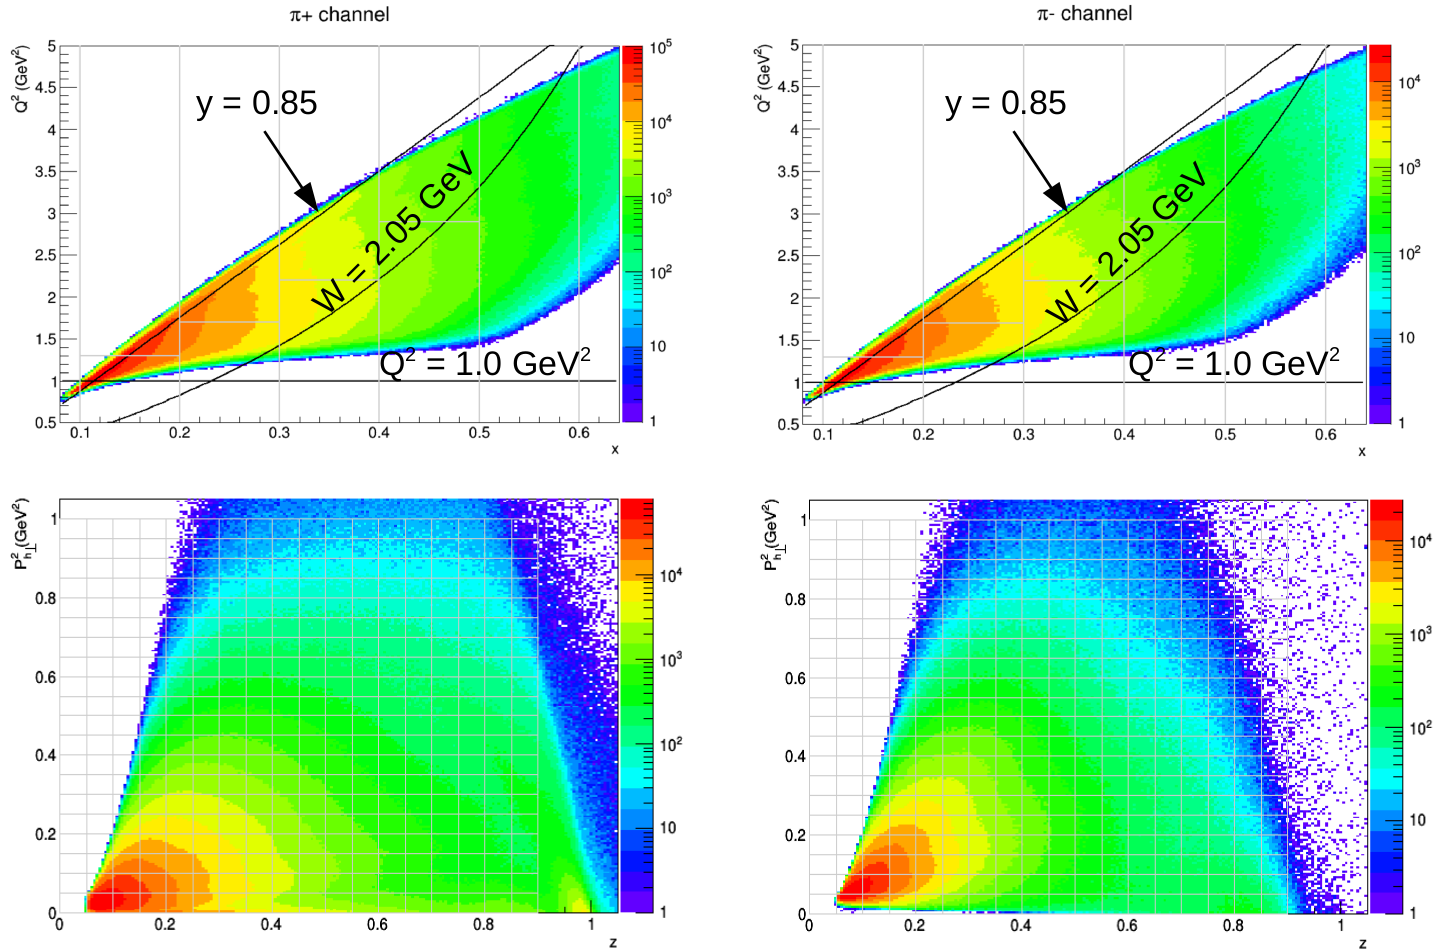
\includegraphics[width=4.5in]{figures/binningScheme.png}
\caption{The $x$-$Q^2$ (top) and $z$-$P_{h\perp}^2$ (bottom) kinematic coverage and binning scheme (gray lines) for $\pi^+$ (left) and $\pi^-$ (right) for the E1-f data set.}
\label{fig:binningScheme}
\end{figure}



\clearpage
%
\chapter{Electron Identification}
\label{cha:eID}
%
Electrons are identified by putting each negative track for a given event through a series of nine cuts.
A candidate electron is considered a ``good'' electron only if it passes all nine cuts.
If an event has more than one good electron, the highest momentum one is chosen.
The nine cuts, described in detail in the subsequent sections, are: matching cuts on the $\theta$ and $\phi$ angles in the CC, a $\theta$ vs $\phi$ fiducial cut, a momentum dependent cut on the EC energy, a cut on the energy in the inner EC, a geometric cut on the EC, fiducial cuts on regions 1 and 3 of the DC, and a cut on the z vertex.
%

\section{CC $\theta$ Matching}
\label{sec:CCthetaMatching}
%
Due to the geometry of the CC, the correspondence between polar angle in the CC, $\theta_{CC}$, and the CC segment number for scattered electrons is manifestly surjective.
A cut is therefore applied on $\theta_{CC}$ for each segment of the CC by fitting the $\theta_{CC}$ distribution with a gaussian plus a polynomial background; events within 3$\sigma$ of the mean pass the cut, see figure~\ref{fig:CCseg_c1}.
%
\begin{figure}[htp]
\centering
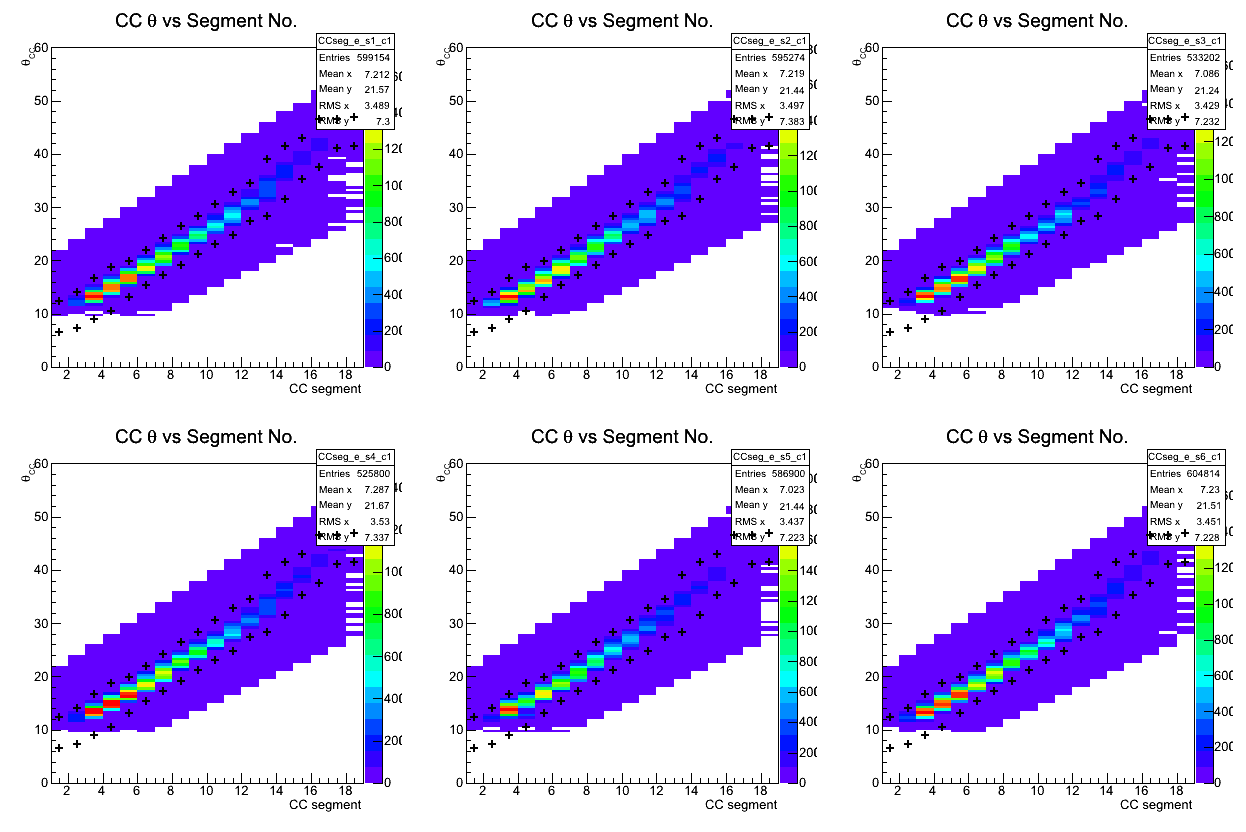
\includegraphics[width=5in]{figures/CCseg_c1.png}
\caption{$\theta_{CC}$ vs CC segment number for each of the six sectors of CLAS. These plots already have the other eight cuts applied and the current cut is given by the black crosses.}
\label{fig:CCseg_c1}
\end{figure}
%
%
\section{CC $\phi$ Matching}
\label{sec:CCphiMatching}
%
Each sector of the CC is divided in half such that each side is a mirror image of the other.
If a track is on one side of the sector but the PMT that fired was on the other side, then the event was likely background and not a good event.
A CC $\phi$ matching algorithm is used that returns 0 if both PMTs fire, $\pm$1 if the track and PMT are on the same side, and $\pm$2 if the track and PMT are on opposite sides.
Events that return $\pm$2 are rejected, all other events are kept.
See figures~\ref{fig:CCphiMatch_c0}~and~\ref{fig:CCphiMatch_c1}.
%
\begin{figure}[htp]
\centering
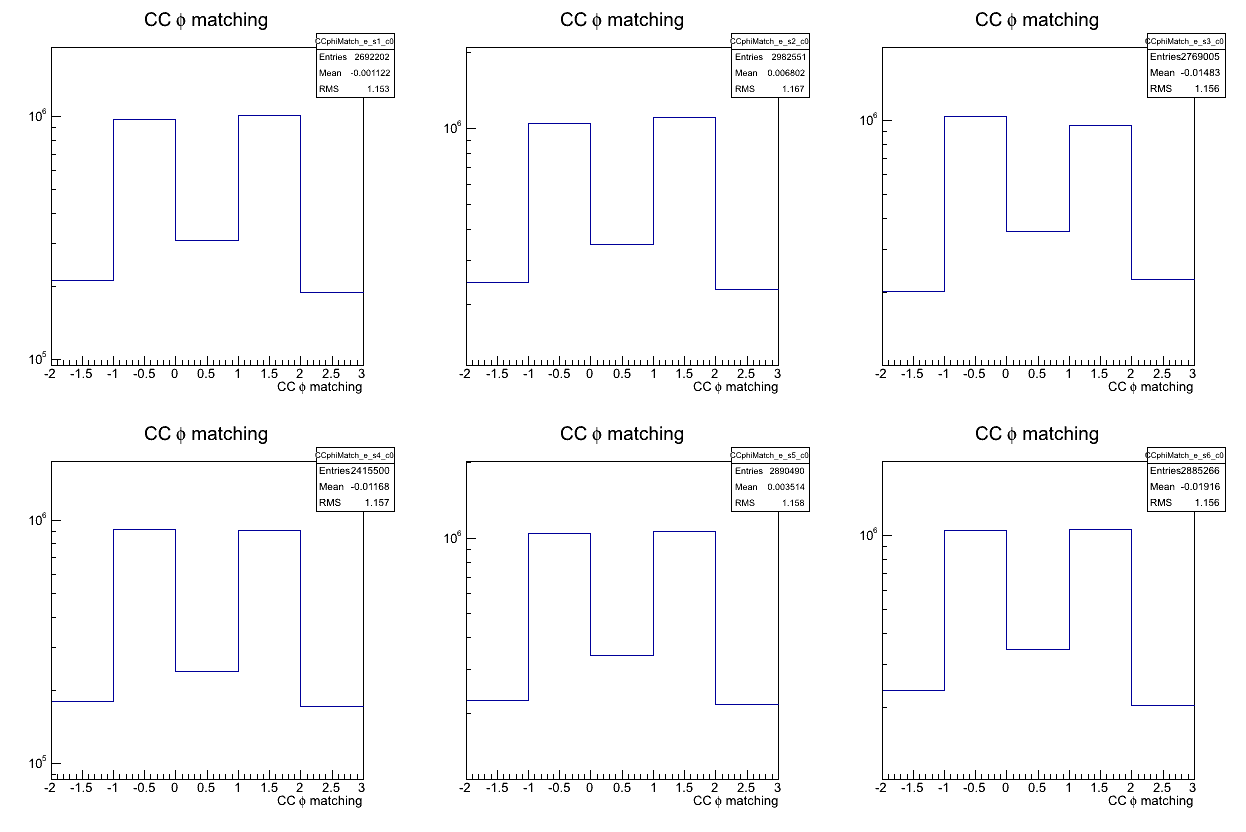
\includegraphics[width=5in]{figures/CCphiMatch_c0.png}
\caption{CC $\phi$ matching distribution for negative tracks for each sector. The matching algorithm returns 0 if both PMTs fire, $\pm$1 if the track and PMT are on the same side, and $\pm$2 if the track and PMT are on opposite sides.}
\label{fig:CCphiMatch_c0}
\end{figure}
%
\begin{figure}[htp]
\centering
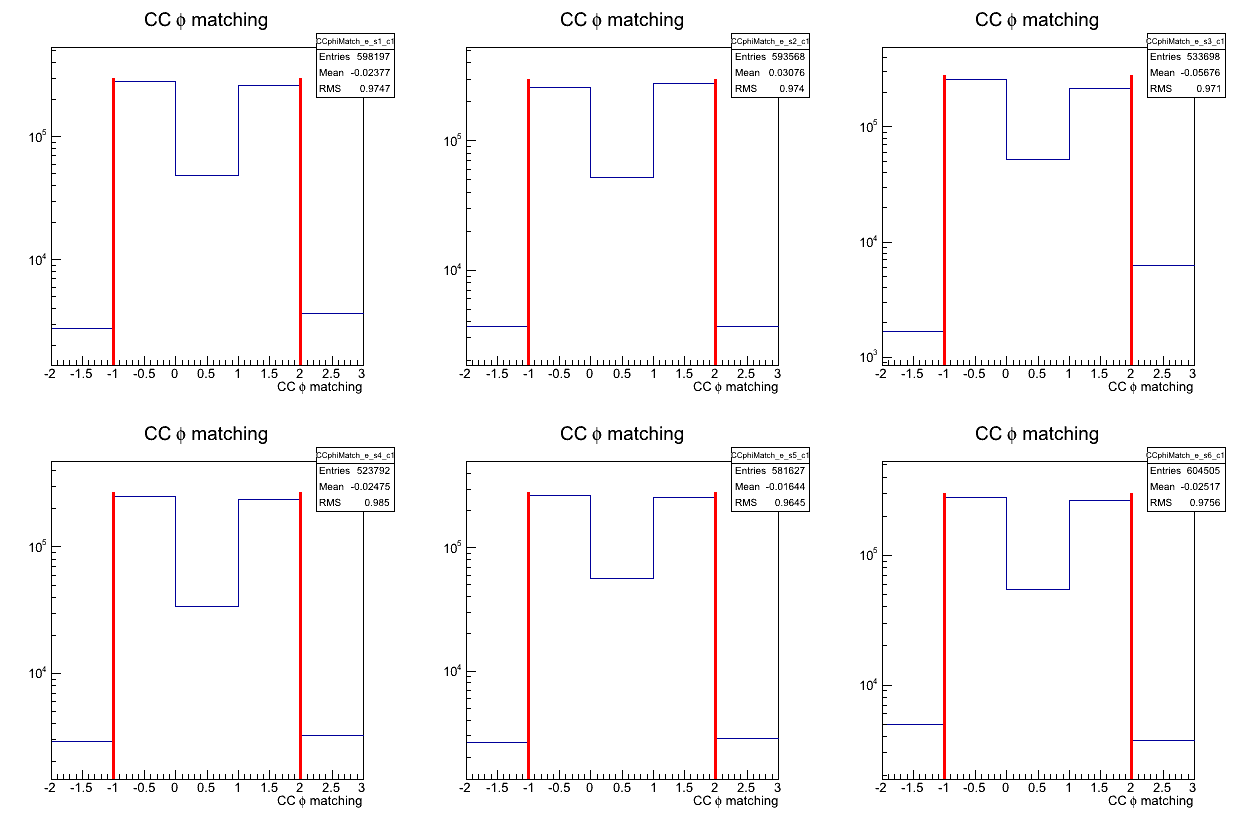
\includegraphics[width=5in]{figures/CCphiMatch_c1.png}
\caption{CC $\phi$ matching distribution for electron candidates with all other electron ID cuts applied for each sector. This cut is shown in red and removes candidate electrons for which the PMT and track are on opposite sides of the sector.}
\label{fig:CCphiMatch_c1}
\end{figure}
%
%
\section{CC Fiducial Cut}
\label{sec:CCfiducial}
%
A geometric cut of the form $\theta_{CC} > 46.0 - 35\sqrt{1 - \frac{\phi^{2}}{350}}$ (units of degrees) is applied to the CC.
The equation was obtained empirically based on the $\theta_{CC}$ vs $\phi$ (lab angle) distribution with and without other electron ID cuts applied.
%See figures~\ref{fig:CCfid_c0}~and~\ref{fig:CCfid_c1}.
See figure~\ref{fig:CCfid_c0c1_6sects}.
%
\begin{sidewaysfigure}[htp]
\centering
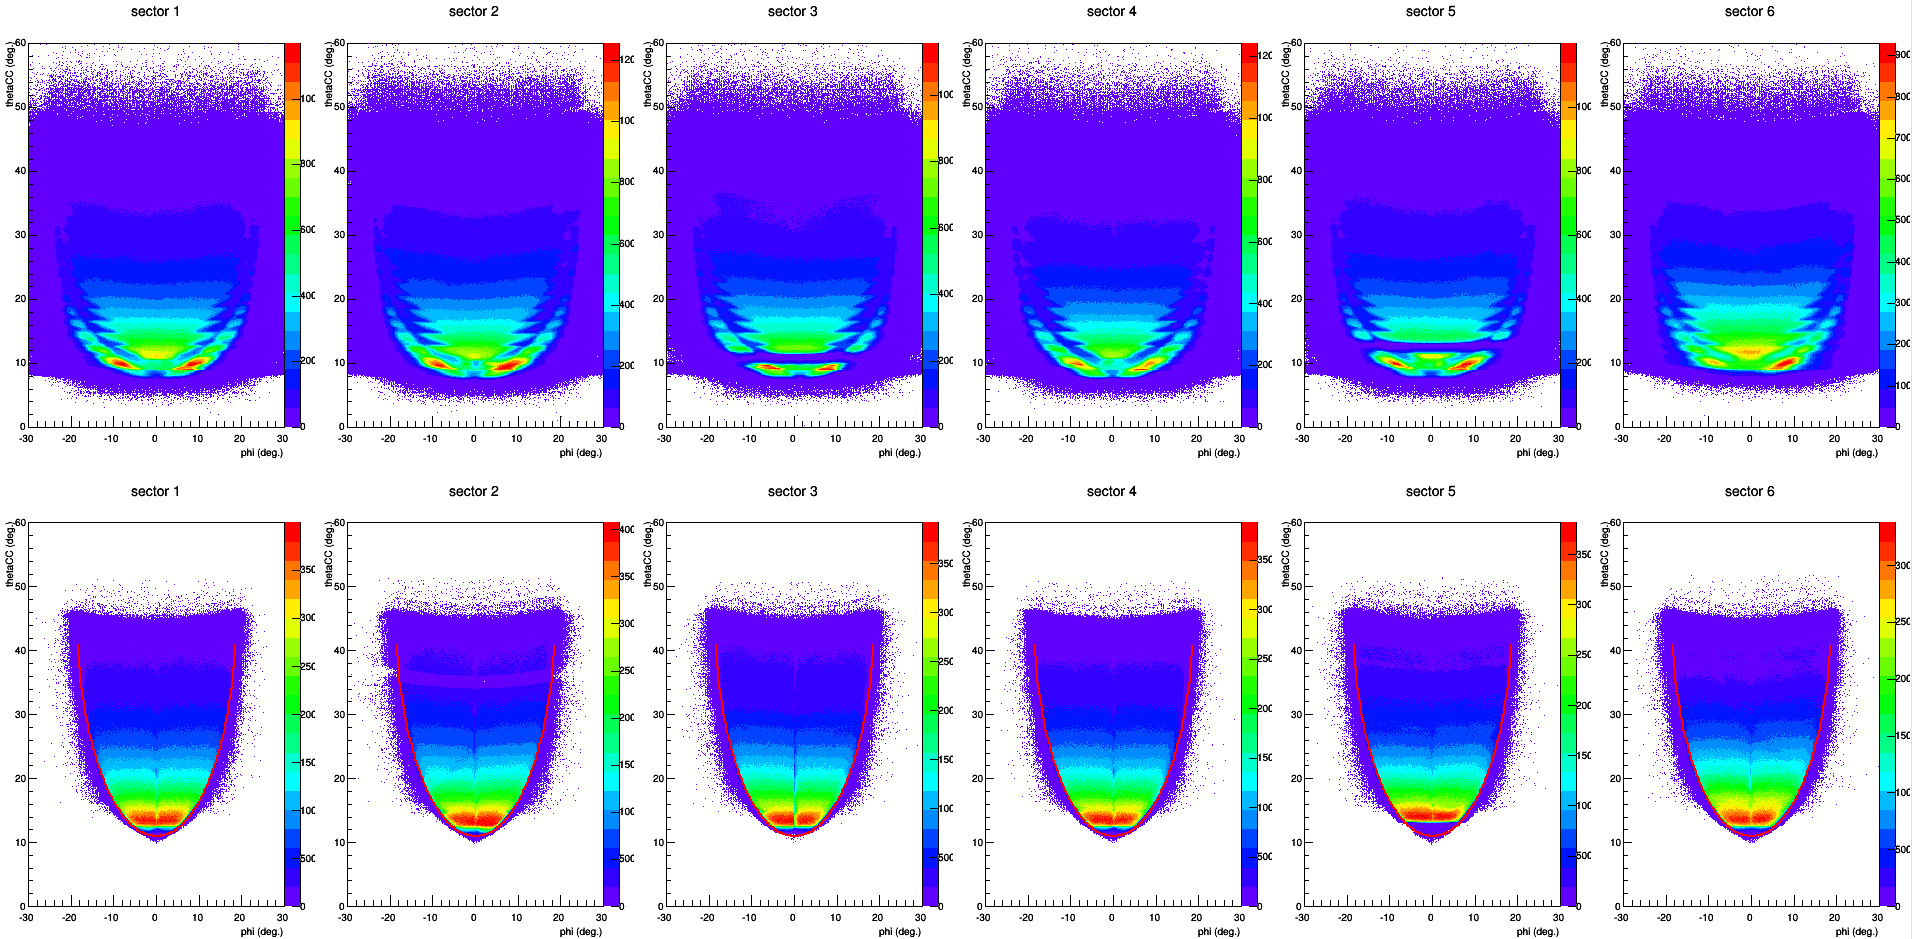
\includegraphics[width=8.5in]{figures/CCfid_c0c1_6sects.png}
\caption{$\theta_{CC}$ vs $\phi$ (lab angle) for each of the six CLAS sectors. The top row shows all negative tracks and the bottom row shows negative tracks which pass all the other electron ID cuts with this cut shown in red.}
\label{fig:CCfid_c0c1_6sects}
\end{sidewaysfigure}
%
%
\section{EC $E_{in}$ vs $E_{out}$ Cut}
\label{sec:ECinvsout}
%
The EC can be used to separate negatively charged pions from electrons in several ways.
Firstly, the scattered electron always travels in a forward direction while pions can have any direction; since the EC only covers forward angles, any track not producing a signal in the EC is immediately rejected.
Secondly, any pion over 0.5 GeV is minimum ionizing in the EC and produces less light in the PMTs than electrons do.
Therefore, only candidate electrons with an energy in the inner part of the EC greater than 0.06 GeV are kept (see figure~\ref{fig:ECoutVinPlot}).
%
\begin{figure}[htp]
\centering
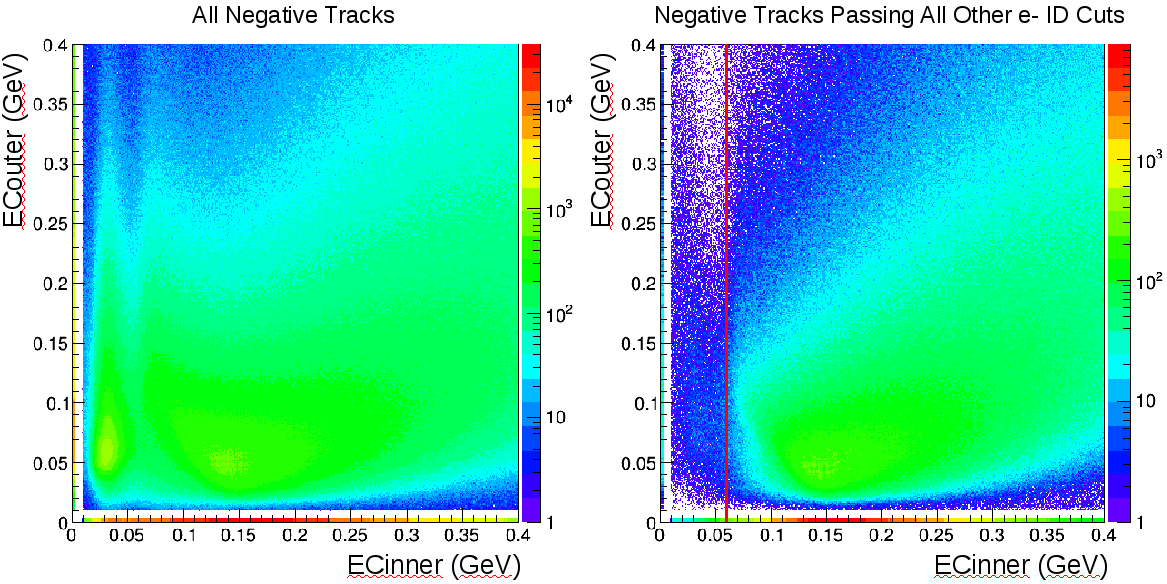
\includegraphics[width=6in]{figures/ECoutVinPlot.png}
\caption{outer EC energy vs inner EC energy plots for (left) all negative tracks and (right) negative tracks passing all other electron ID cuts. Tracks with and inner EC energy greater than 0.06 GeV pass this cut (shown by the red line in the plot on the right).}
\label{fig:ECoutVinPlot}
\end{figure}
%
\section{EC Sampling Fraction Cut}
\label{sec:ECsampling}
%
The ratio of total energy to momentum stays nearly constant as a function of momentum for electrons.
To eliminate background as well as contamination from other negative tracks, each momentum bin is fit with a gaussian and the points at $\mu + 5\sigma$ and $\mu - 3\sigma$ are fit with a second order polynomial to define the cut.
Figure~\ref{fig:ECsampling_c0c1_6sects} shows the E/p vs p distribution candidate electrons along with the cut described here.
%
\begin{sidewaysfigure}[htp]
\centering
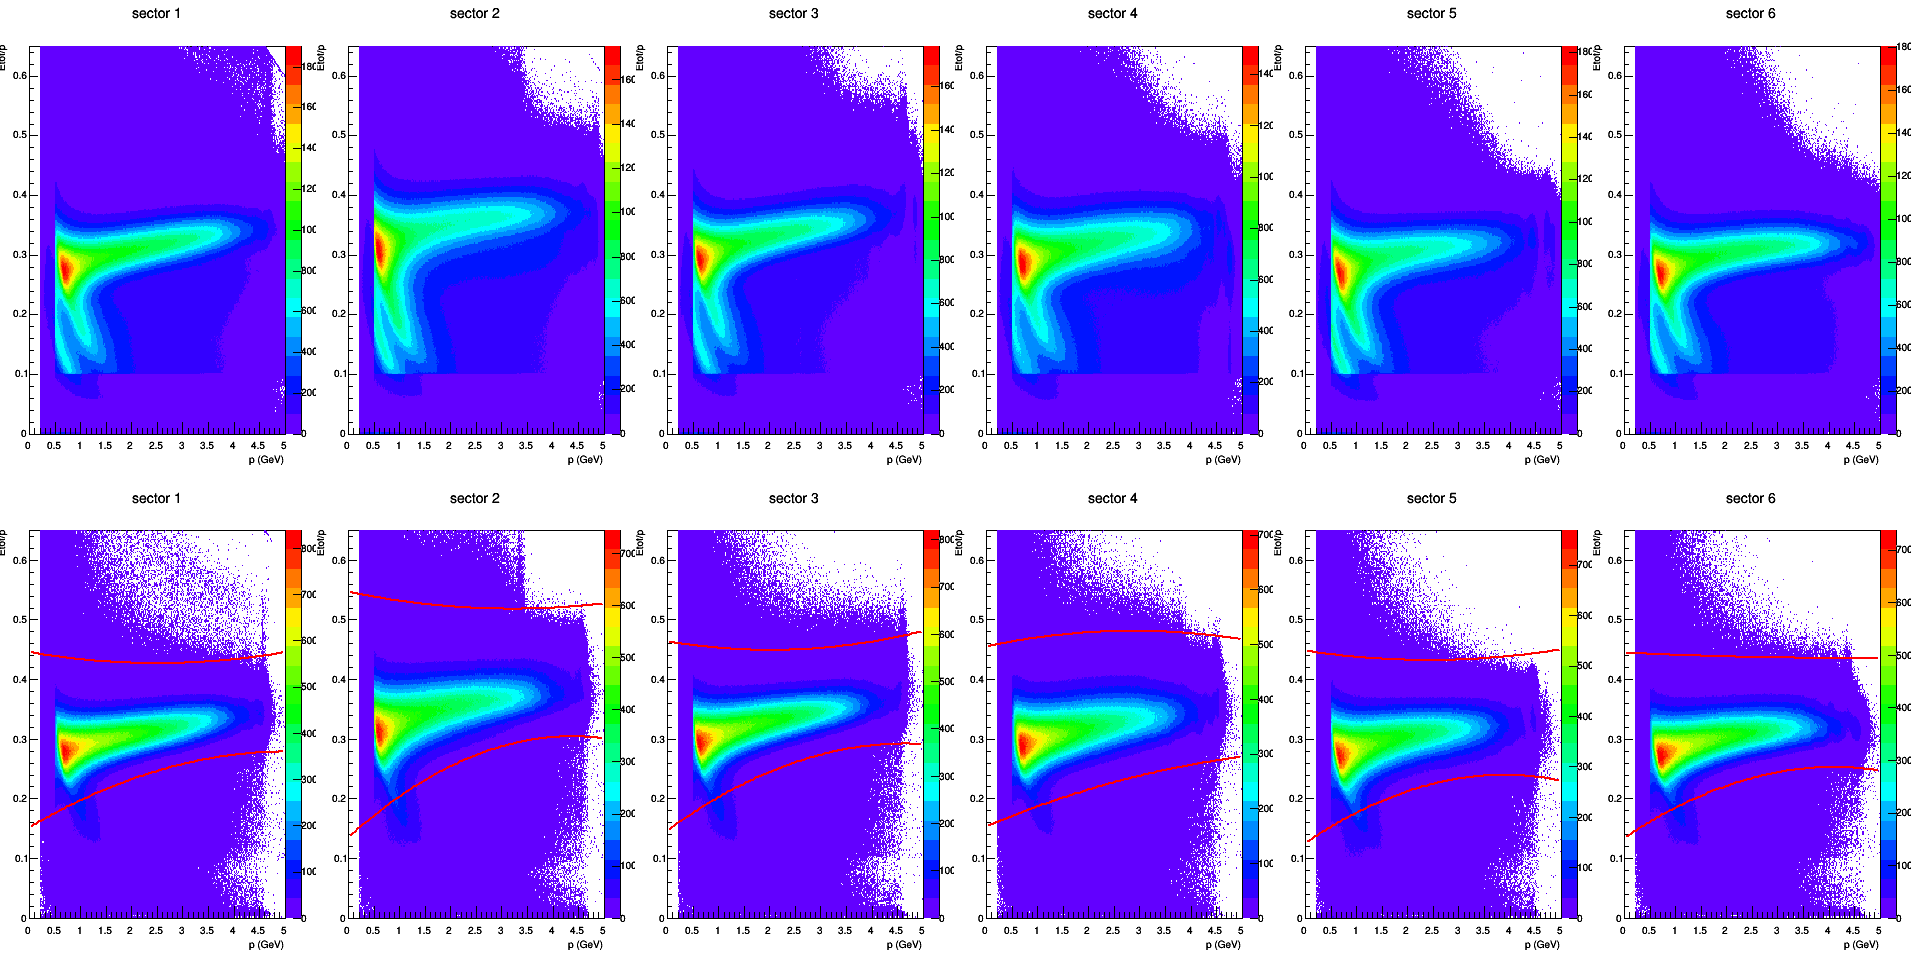
\includegraphics[width=8.5in]{figures/ECsampling_c0c1_6sects.png}
\caption{The energy deposited in the EC divided by momentum as a function of momentum for electron candidates for each of the six CLAS sectors. The top row shows all negative tracks and the bottom row shows the tracks passing all other electron ID cuts with this cut shown in red.}
\label{fig:ECsampling_c0c1_6sects}
\end{sidewaysfigure}
%
%
\section{EC Geometric Cut}
\label{sec:ECgeometric}
%
When a particle deposits its energy in the EC a ``shower'' is created.
If this shower occurs close to the edge of one of the EC triangles only a fraction of the particle's energy is reconstructed.
Since energy information about these particles is unreliable they are cut via a geometric cut on the EC (see figure~\ref{fig:ECgeometricPlot}).
%
\begin{figure}[htp]
\centering
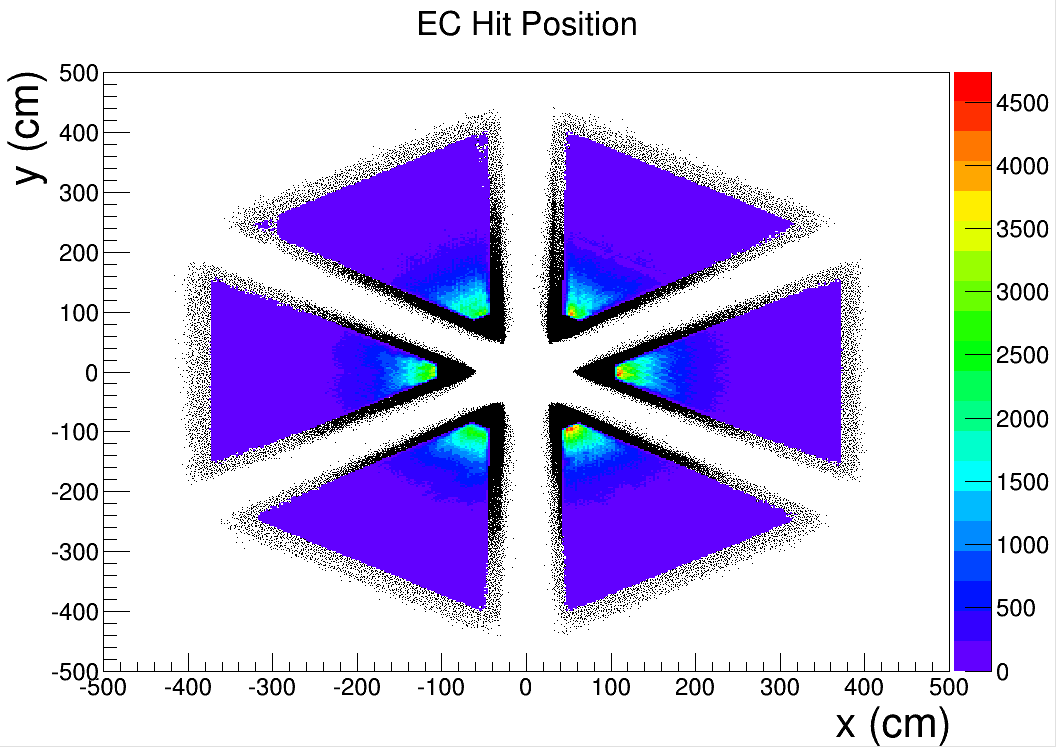
\includegraphics[width=5in]{figures/ECgeometricPlot.png}
\caption{The distribution of hits in the EC. The black points show the hit positions for all negative tracks and the colored points show the hit positions for the final electron sample. It can clearly be seen that tracks hitting near any of the edges have been removed.}
\label{fig:ECgeometricPlot}
\end{figure}
%
%
\section{Region 1 Fiducial Cut}
\label{sec:R1fid}
%
A geometric fiducial cut is applied to X-Y position of tracks in region 1 of the DC.
The cut is shown with red lines in figure~\ref{fig:R1fid_c0c1_6sects}.
The lines are symmetric about Y=0, form a $60^\circ$ angle, and intersect at X=22 cm.
These cuts were chosen to approximately respect the geometry of the DC.
%
\begin{sidewaysfigure}[htp]
\centering
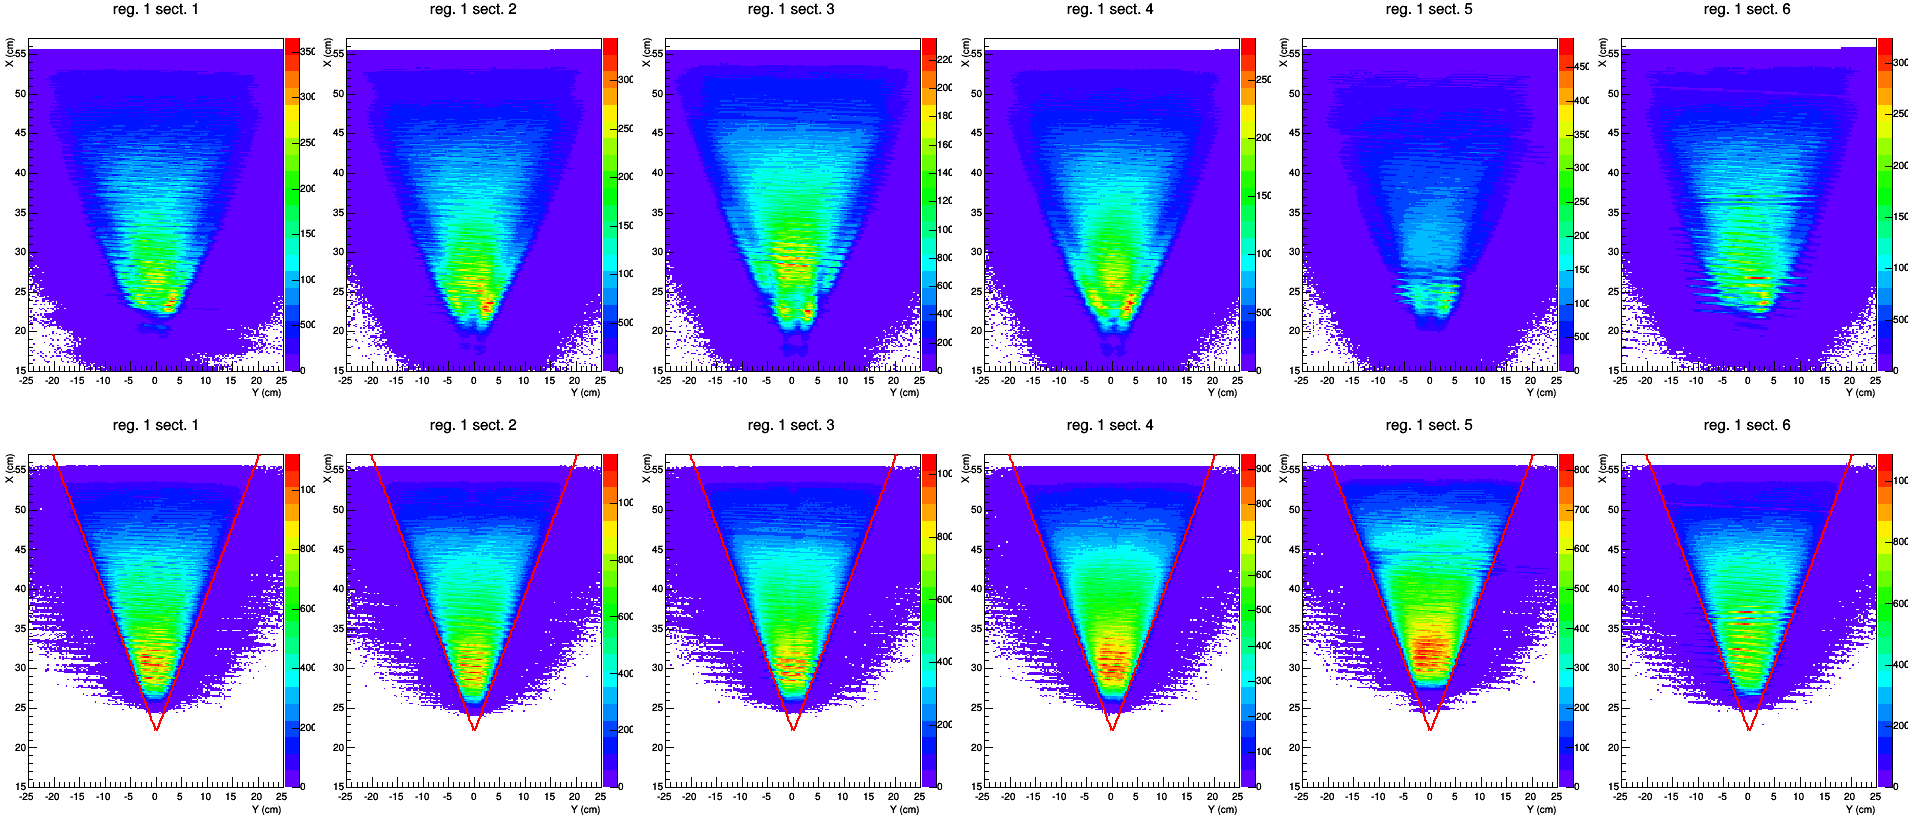
\includegraphics[width=8.5in]{figures/R1fid_c0c1_6sects.png}
\caption{The X vs Y position of tracks in region 1 of the DC for each sector. The top row shows results for all negative tracks and the bottom row shows results with all the other electron ID cuts applied. The cut applied here is shown with red lines.}
\label{fig:R1fid_c0c1_6sects}
\end{sidewaysfigure}
%
%
\section{Region 3 Fiducial Cut}
\label{sec:R3fid}
%
A geometric fiducial cut is applied to X-Y position of tracks in region 3 of the DC.
The cut is shown with red lines in figure~\ref{fig:R3fid_c0c1_6sects}.
The lines are symmetric about Y=0, form a $49^\circ$ angle, and intersect at X=83 cm.
These cuts were chosen to approximately respect the geometry of the DC.
%
\begin{sidewaysfigure}[htp]
\centering
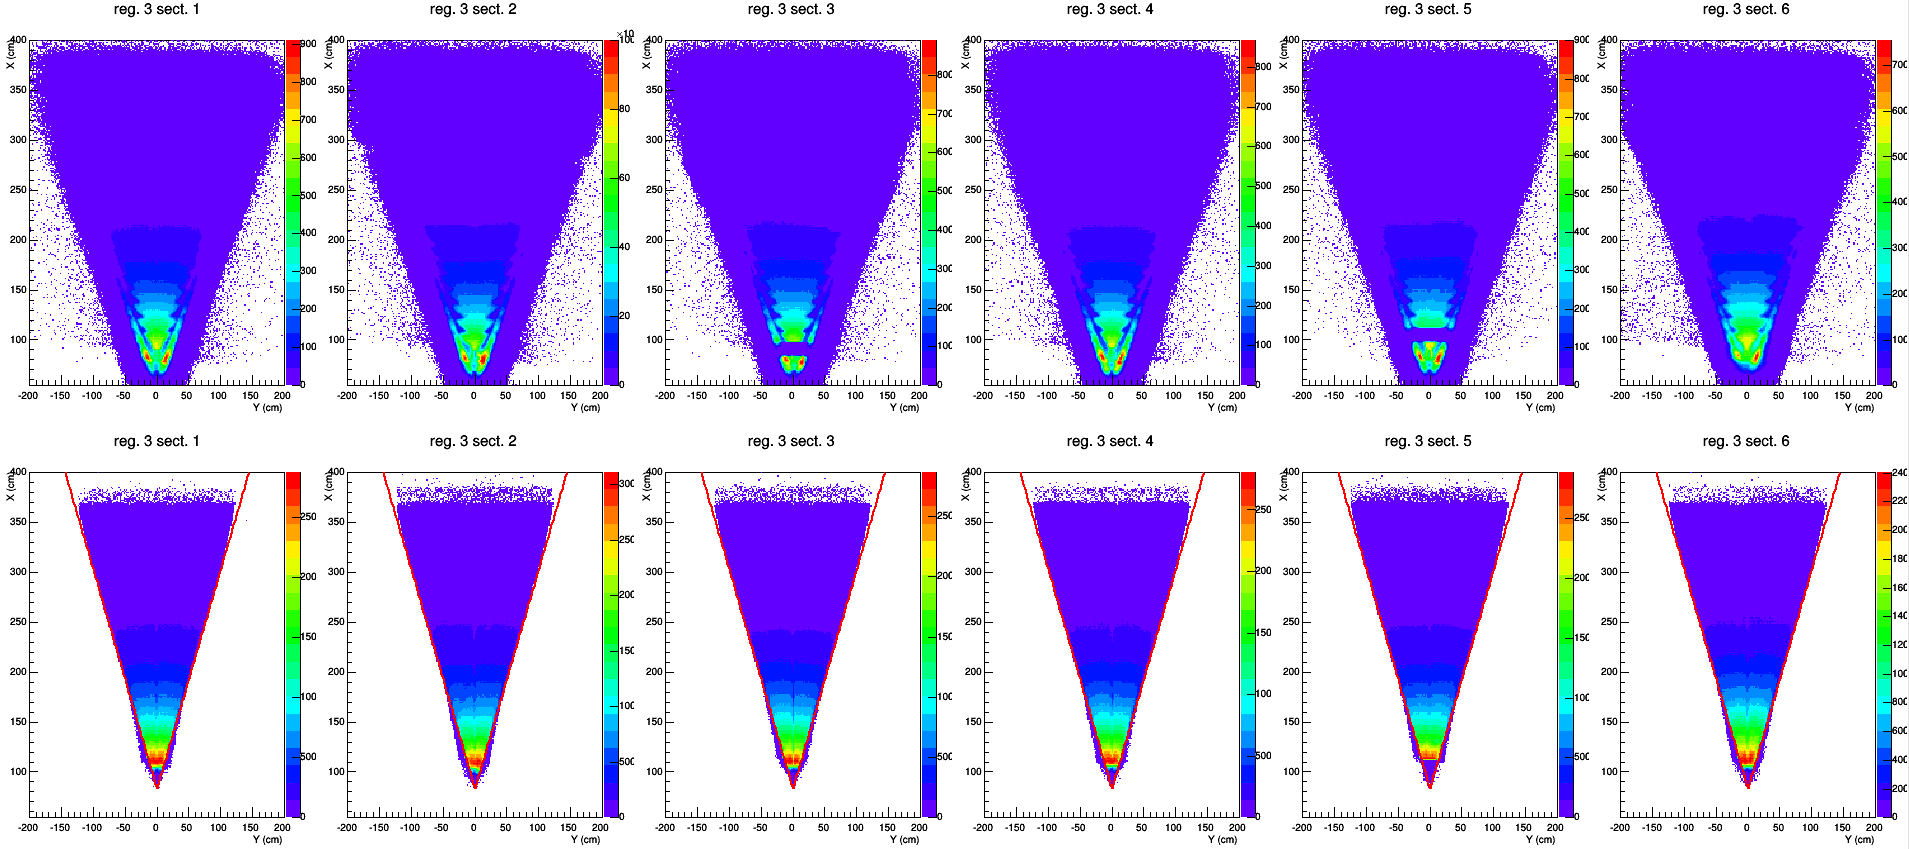
\includegraphics[width=8.5in]{figures/R3fid_c0c1_6sects.png}
\caption{The X vs Y position of tracks in region 3 of the DC for each sector. The top row shows results for all negative tracks and the bottom row shows results with all the other electron ID cuts applied. The cut applied here is shown with red lines.}
\label{fig:R3fid_c0c1_6sects}
\end{sidewaysfigure}
%

\section{z Vertex Correction and Cut}
\label{sec:zvertexCorrAndCut}
%
A cut is made on the z vertex to remove candidates that do not originate from the target.
The efficacy of the cut can be improved by first applying a vertex correction.
During reconstruction, a vertex $(x, y, z)$ is calculated for each charged track based on the intersection of the track with the midplane of the corresponding sector.
The midplane of a sector is the plane that divides the sector in half and contains the supposed beamline $(0, 0, z)$.
However, during the E1-f experiment the beam was not centered at $(x, y) = (0, 0)$, therefore a correction to the z vertex is applied.
Figure~\ref{fig:xyBeamOffset} shows the $(x, y)$ offset of the beam; events in this plot were selected from the aluminium foil located downstream from the target to fix the $z$ position.
The calculated value for the beam position is $(x, y) = (0.15 cm, -0.25 cm)$.

% the blank line above is on purpose to end the paragraph
\begin{figure}[htp]
\centering
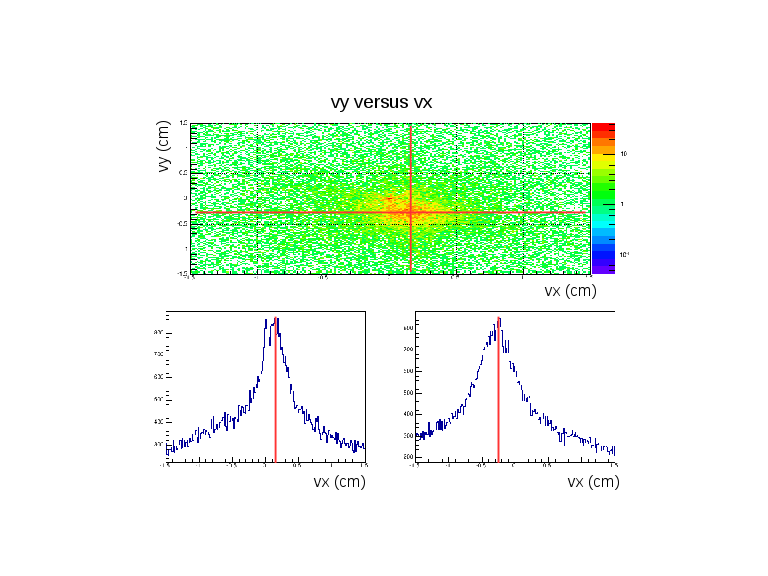
\includegraphics[width=6in, trim={1cm 1cm 1cm 1cm}, clip]{figures/xyBeamOffset.png}
\caption{Top: y vs x beam position for the E1-f run. Bottom left: x beam position for the E1-f run. Bottom right: y beam position for the E1-f run. The beam position is located at $x = 0.15 cm, y = -0.25 cm$ which is indicated by the red lines.}
\label{fig:xyBeamOffset}
\end{figure}
%
The z vertex is corrected by recalculating the intersection of the tracks with the midplanes after shifting the midplanes so that they contain the correct beamline $(0.15, -0.25, z)$.
The z vertex for electron candidates is plotted in figure~\ref{fig:corrVuncorrZvertex} before and after applying the correction.

% the blank line above is on purpose to end the paragraph
\begin{figure}[htp]
\centering
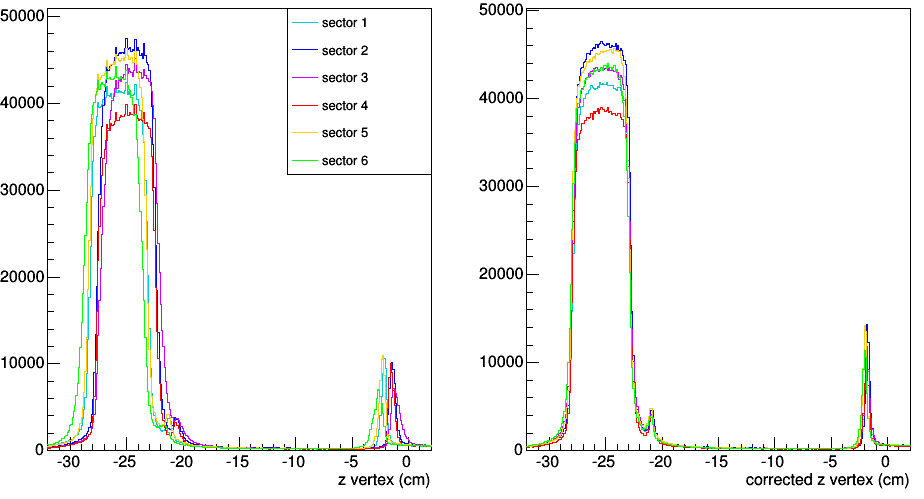
\includegraphics[width=6in]{figures/corrVuncorrZvertex.png}
\caption{Left: The z vertex for electron candidates for each sector. Right: The corrected z vertex for electron candidates for each sector. The two peaks near $-21 cm$ and $-2 cm$ are from aluminium foils placed there as reference points.}
\label{fig:corrVuncorrZvertex}
\end{figure}
%
The E1-f experiment was designed to have a $5 cm$ long target centered at $z = -25 cm$.
To have an even more precise location of the target, empty target runs are used to identify the positions of the target cell's entry and exit window (see figure~\ref{fig:emptyTargZ_integ6}).
The target cell's entry window was measured to be at $z = -27.7302 cm$ and the exit window was measured to be at $z = -22.6864 cm$; these values are used for the electron z vertex cut, which is shown in figure~\ref{fig:e_zvertexCut}.
%
\begin{figure}[htp]
\centering
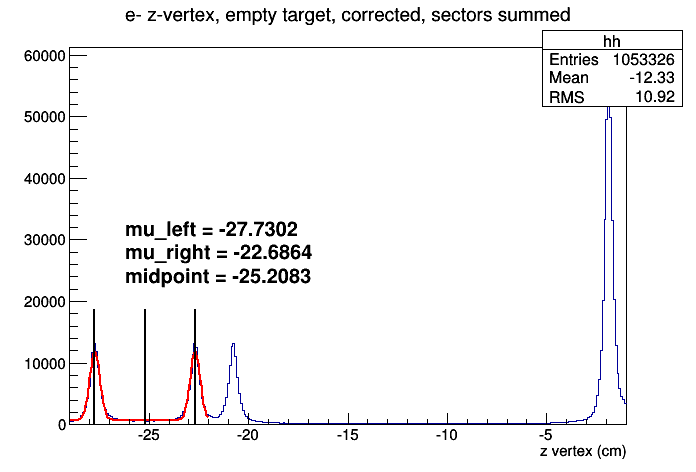
\includegraphics[width=4in]{figures/emptyTargZ_integ6.png}
\caption{The electron z vertex distribution for empty target runs. This data is used to identify the precise location of the target cell's entry and exit window. The two peaks near $-21 cm$ and $-2 cm$ are from aluminium foils placed there as reference points.}
\label{fig:emptyTargZ_integ6}
\end{figure}
%
\begin{figure}[htp]
\centering
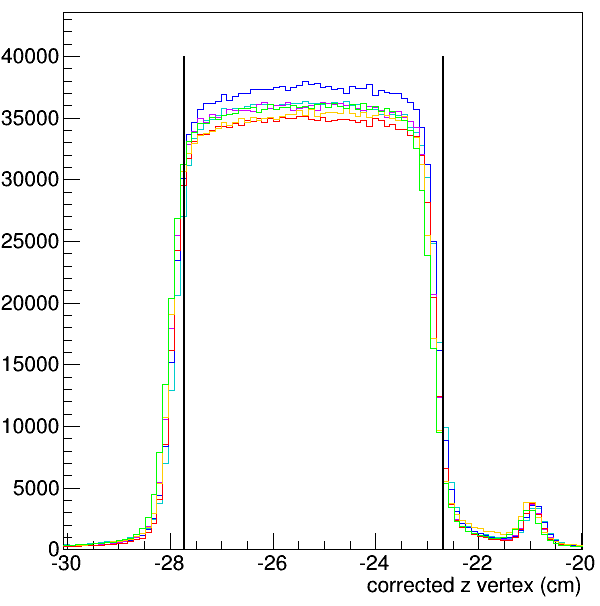
\includegraphics[width=3in]{figures/e_zvertexCut.png}
\caption{The corrected z vertex distribution for electrons candidates passing all the other electron ID cuts with this cut shown by black vertical lines. The peak near $-21 cm$ is from an aluminium foil placed there as a reference point.}
\label{fig:e_zvertexCut}
\end{figure}
%
\clearpage

\chapter{Hadron Identification}
\label{cha:hadronID}
%
\section{$\pi^+$ Identification}
\label{sec:pipID}
Positive pions are identified by selecting positive tracks that pass a momentum and sector dependent $\beta$ cut (where $\beta = v/c$).
Additionally, a geometric fiducial cut is applied to region 1 of the DC.
A missing mass cut is also applied.
Traditionally, missing mass cuts are used for selecting particular kinematic regions, not for particle ID.
However, in this situation a missing mass cut significantly improved $\pi^+$/proton separation, and since SIDIS event selection requires a missing mass cut anyway, this cut is applied at the particle ID stage.
%
\subsection{$\pi^+$ Missing Mass Cut}
In pion SIDIS events ($ep \rightarrow e\pi X$), the missing mass ($M_X$) is defined as the invariant mass of the undetected state $X$.
That is, if $p$, $q$, and $\pi$ are the 4-momenta of the initial state proton, the virtual photon, and the detected pion, respectively, then
\begin{equation}
\label{eq:missingMassDefinition}
M_X^2 = \left( p + q - \pi \right)^2.
\end{equation}
To calculate this the pion mass is assumed for the candidate pion.
Figure~\ref{fig:pipMissingMassCut} shows the $M_X$ distribution for candidate $ep \rightarrow e\pi^+ X$ events.
Events with $M_X < 1.35$ GeV are cut.
This cut helps to remove proton contamination at high momenta, which can be seen in figure~\ref{fig:pip_vvp_beforeAndAfter_MXcut} and also cuts out exclusive events ($ep \rightarrow e\pi^+ n$, the peak near the nucleon mass (0.938 GeV) in figure~\ref{fig:pipMissingMassCut}) and the delta resonance (the peak near 1.2 GeV in figure~\ref{fig:pipMissingMassCut}), both of which are not desirable for a SIDIS sample anyway.
\begin{figure}[htp]
\centering
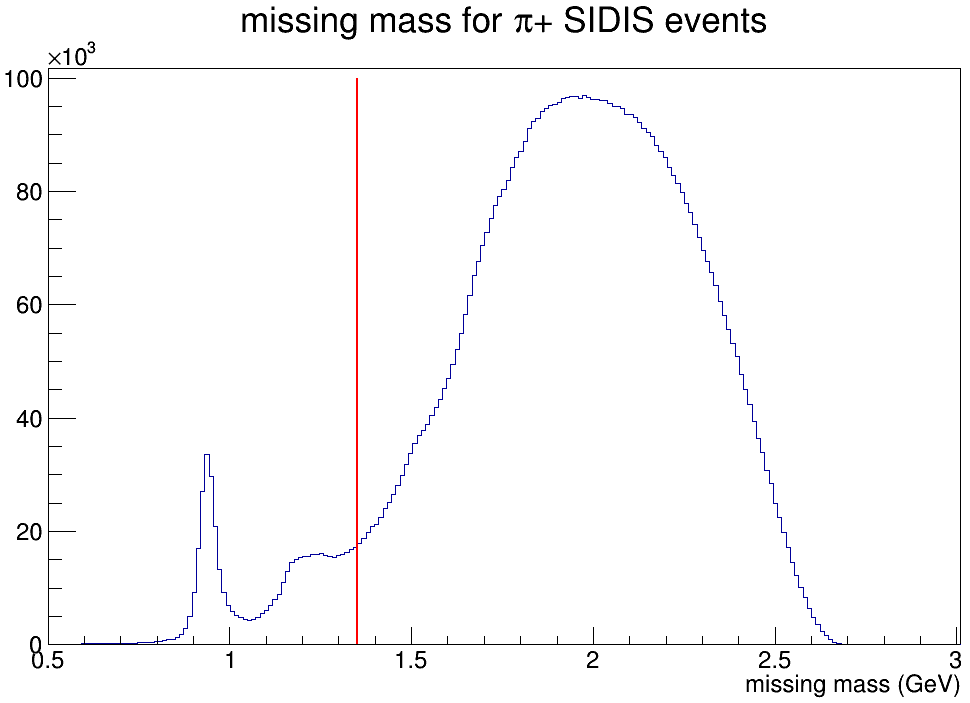
\includegraphics[width=3in]{figures/pipMissingMassCut.png}
\caption{The missing mass distribution for $ep \rightarrow e\pi^+ X$ events. The vertical red line shows the cut of 1.35 GeV. Events to the left of this line are removed from the sample.}
\label{fig:pipMissingMassCut}
\end{figure}
%
\begin{figure}[htp]
\centering
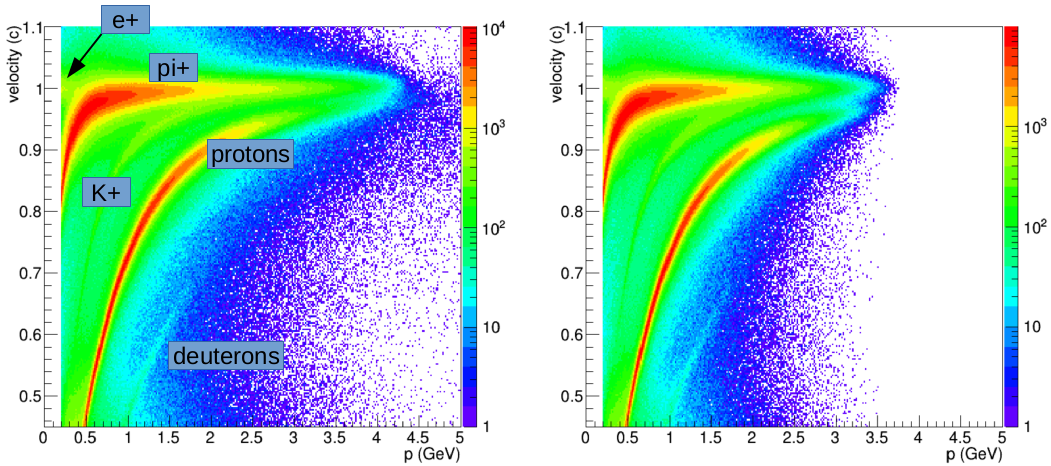
\includegraphics[width=6in]{figures/pip_vvp_beforeAndAfter_MXcut.png}
\caption{$\beta$ vs momentum distribution for positive tracks before (left) and after (right) the missing mass cut. The cut removes most tracks above 3.5 GeV, making $\pi^+$/proton separation easier. SIDIS samples require a missing mass cut anyway, so it makes sense to apply it here at the particle ID stage.}
\label{fig:pip_vvp_beforeAndAfter_MXcut}
\end{figure}
%
\subsection{$\pi^+ \beta$ Cut}
$\beta$ is calculated by simply dividing the track's path length by its time of flight and then dividing this quantity by the speed of light.
To select positive pions, $\beta$ for positive tracks is plotted in 70 bins of momentum from 0.2 to 3.75 GeV (with the missing mass cut applied).
The pion peak for each bin is then fit with a gaussian.
At low momenta, a $3\sigma$ cut is used, while at higher momenta a tighter cut, which was estimated by eye, is used.
The tightening of the cut at higher momenta is clearly necessary to reduce proton contamination.
This is shown (for electron sector 4) in figure~\ref{fig:pos_1Dbeta_pBins} - the top left plot is the lowest momentum bin and the bottom right plot highest momentum bin, the red curves show the gaussian fits, the vertical black lines show $\mu \pm 3\sigma$, and the vertical red lines show the actual cut.
The two dimensional view of this cut is shown in figure~\ref{fig:pip_vvpCut}.

Although some proton contamination remains after this cut, careful Monte Carlo simulations and systematic error studies, described later in this paper, correct for this.
Figure~\ref{fig:pipID_beta_pBins_dataTop_MCbottom} shows a comparison between the E1-f data and Monte Carlo in the momentum region where the contamination is worst.
%
\begin{sidewaysfigure}[htp]
\centering
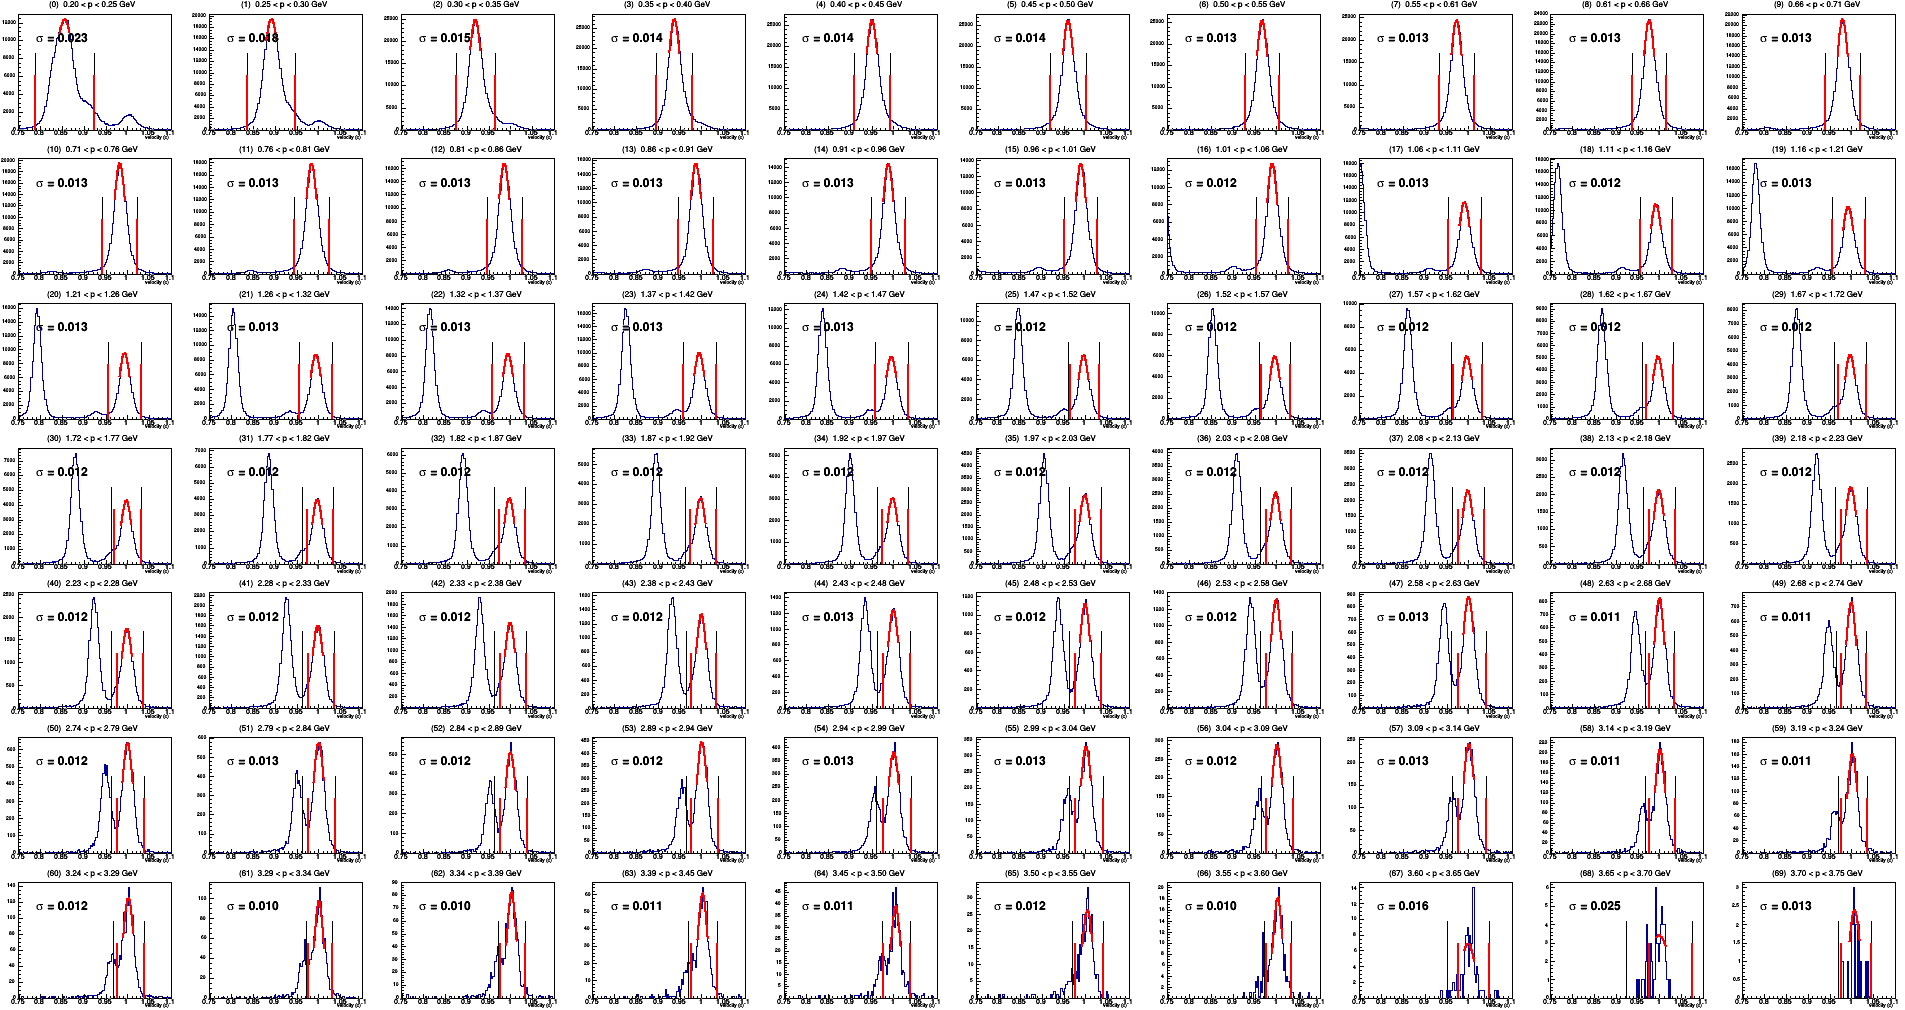
\includegraphics[width=8.5in]{figures/pos_1Dbeta_pBins.png}
\caption{$\beta$ for positive tracks in bins of momentum when the electron is in sector 4. The top left plot is the lowest momentum bin and the bottom right plot highest momentum bin, the red curves show the gaussian fits, the vertical black lines show $\mu \pm 3\sigma$, and the vertical red lines show the actual cut.}
\label{fig:pos_1Dbeta_pBins}
\end{sidewaysfigure}
%
\begin{figure}[htp]
\centering
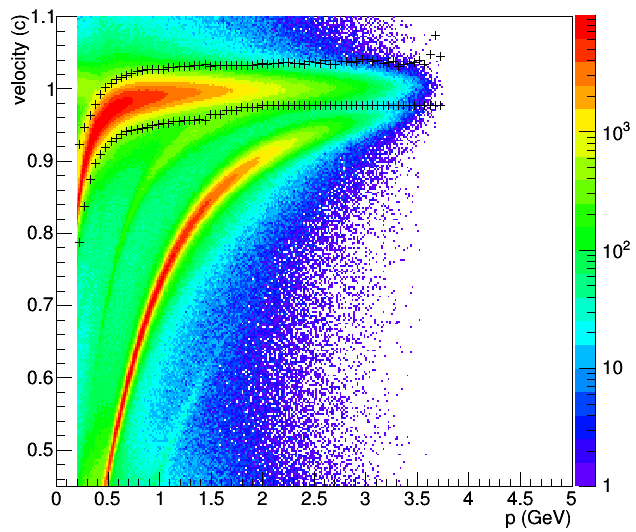
\includegraphics[width=4in]{figures/pip_vvpCut.png}
\caption{The two dimensional view of the $\pi^+$ $\beta$ cut. The black crosses show the upper and lower cut for each of the 70 momentum bins.}
\label{fig:pip_vvpCut}
\end{figure}
%
\begin{figure}[htp]
\centering
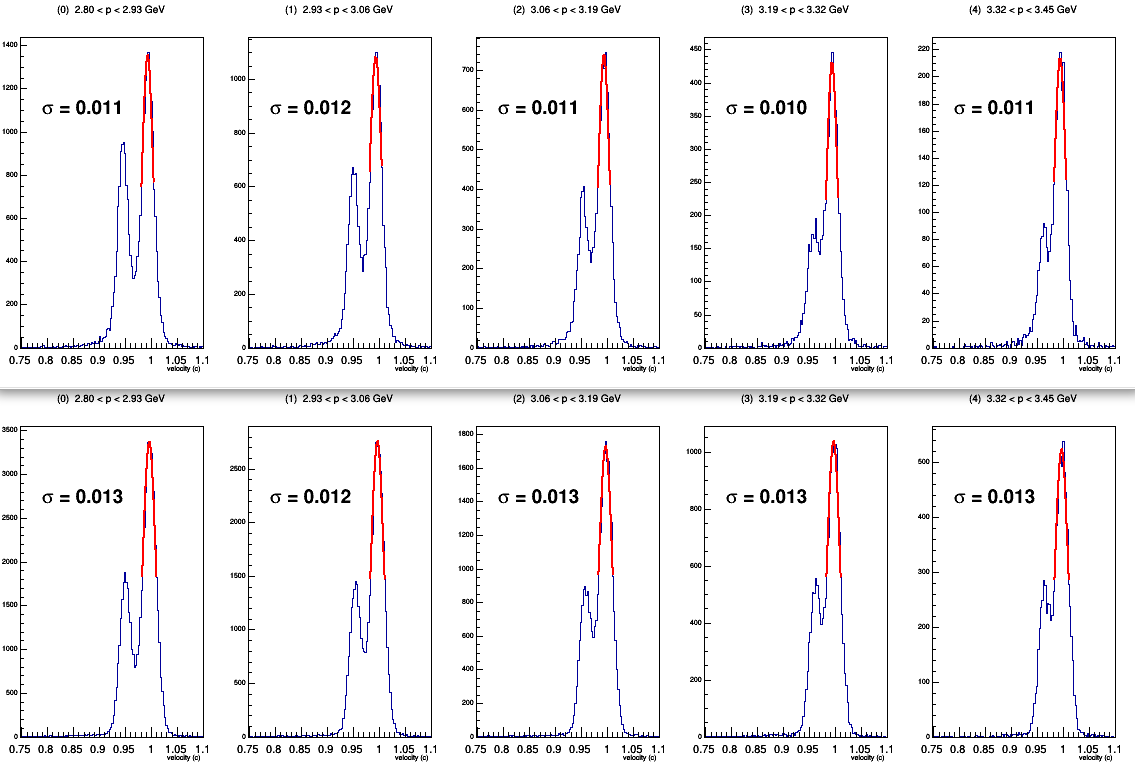
\includegraphics[width=6in]{figures/pipID_beta_pBins_dataTop_MCbottom.png}
\caption{$\beta$ for positive tracks in several momentum bins in the region where proton contamination is worst for data (top row) and Monte Carlo (bottom row).}
\label{fig:pipID_beta_pBins_dataTop_MCbottom}
\end{figure}
%
\subsection{$\pi^+$ Fiducial Cut}
To improve the data quality, a geometric fiducial cut is applied to region 1 of the DC.
The cut is shown with red lines in figure~\ref{fig:pip_R1cut_s4}.
The lines are symmetric and form a $60^\circ$ angle and intersect at $(0, 10)$ cm.
\begin{figure}[htp]
\centering
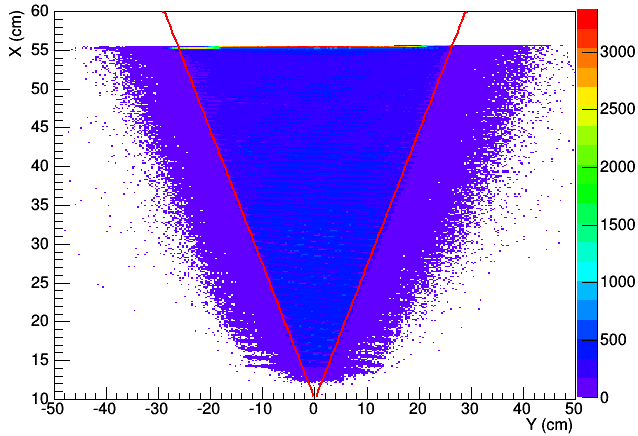
\includegraphics[width=4in]{figures/pip_R1cut_s4.png}
\caption{X vs Y in region 1 of the DC for positive tracks. Events inside of the red lines are kept.}
\label{fig:pip_R1cut_s4}
\end{figure}
%
%

\clearpage % should prevent a backlog of figures from piling up

%
%
\section{$\pi^-$ Identification}
\label{sec:pimID}
Negative tracks that are not identified as electrons become $\pi^-$ candidates.
Negative pions are then selected using cuts very similar to the $\pi^+$ ID.
%
\subsection{$\pi^-$ Missing Mass Cut}
Although the $\pi^-$ channel does not have proton (or anti-proton) contamination, a missing mass cut of 1.35 GeV is applied here as well for consistency.
Figure~\ref{fig:pimMissingMassCut} shows this cut.
%
\begin{figure}[htp]
\centering
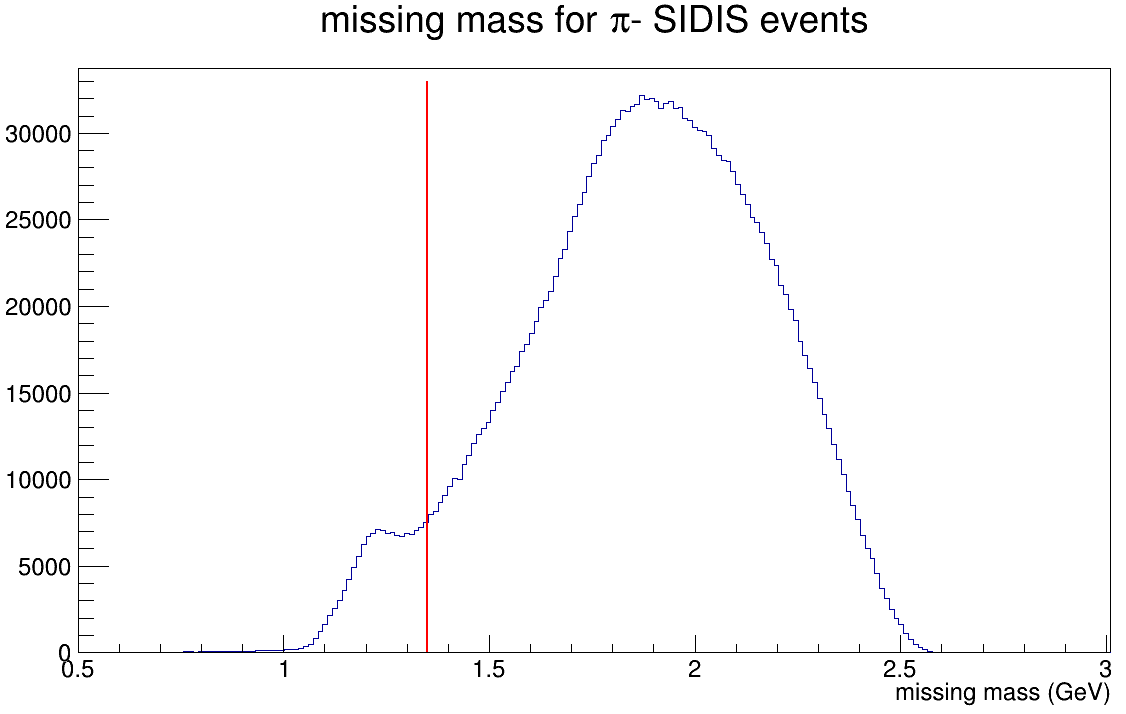
\includegraphics[width=3in]{figures/pimMissingMassCut.png}
\caption{The missing mass distribution for $ep \rightarrow e\pi^- X$ events. The vertical red line shows the cut of 1.35 GeV. Events to the left of this line are removed from the sample.}
\label{fig:pimMissingMassCut}
\end{figure}
%
\subsection{$\pi^- \beta$ Cut}
The $\pi^-$ $\beta$ cut is done in exactly the same way as $\pi^+$ $\beta$ cut.
The results can be seen in figures~\ref{fig:neg_1Dbeta_pBins} and~\ref{fig:pim_vvpCut}.
%
\begin{sidewaysfigure}[htp]
\centering
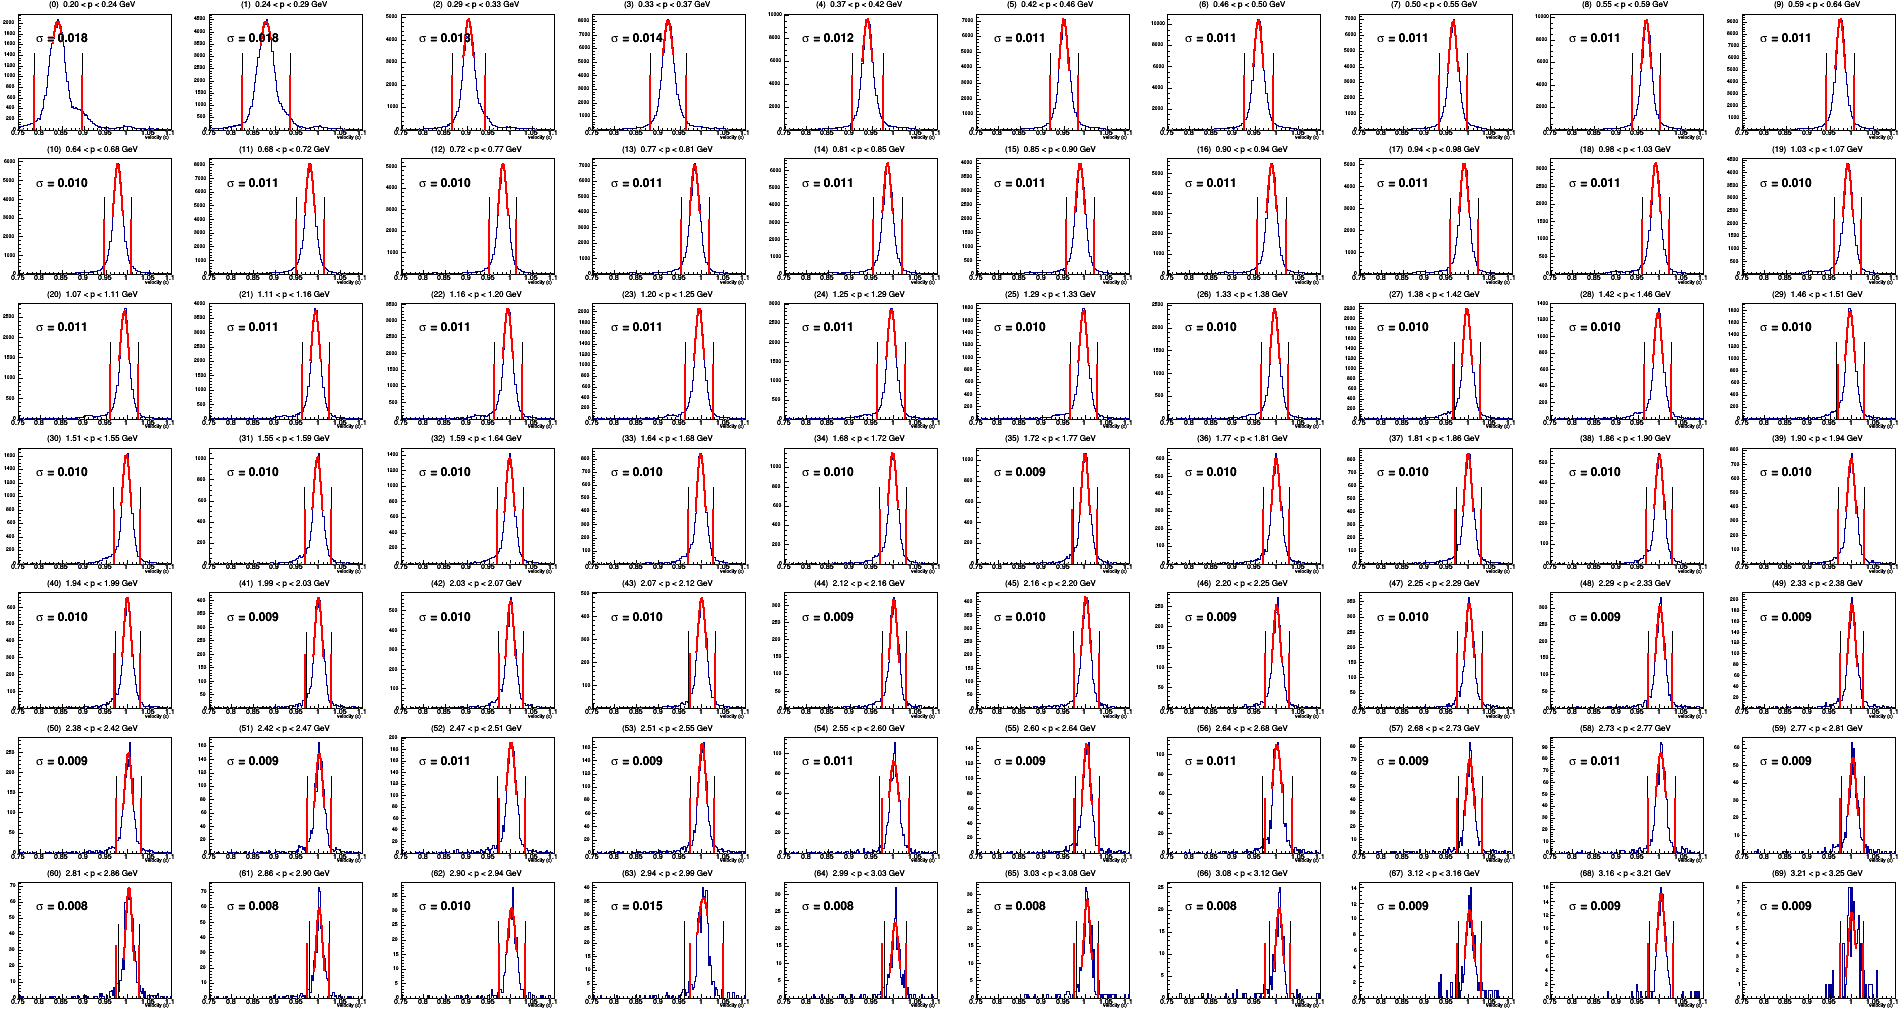
\includegraphics[width=8.5in]{figures/neg_1Dbeta_pBins.png}
\caption{$\beta$ for negative tracks in bins of momentum when the electron is in sector 3. The top left plot is the lowest momentum bin and the bottom right plot highest momentum bin, the red curves show the gaussian fits, the vertical black lines show $\mu \pm 3\sigma$, and the vertical red lines show the actual cut.}
\label{fig:neg_1Dbeta_pBins}
\end{sidewaysfigure}
%
\begin{figure}[htp]
\centering
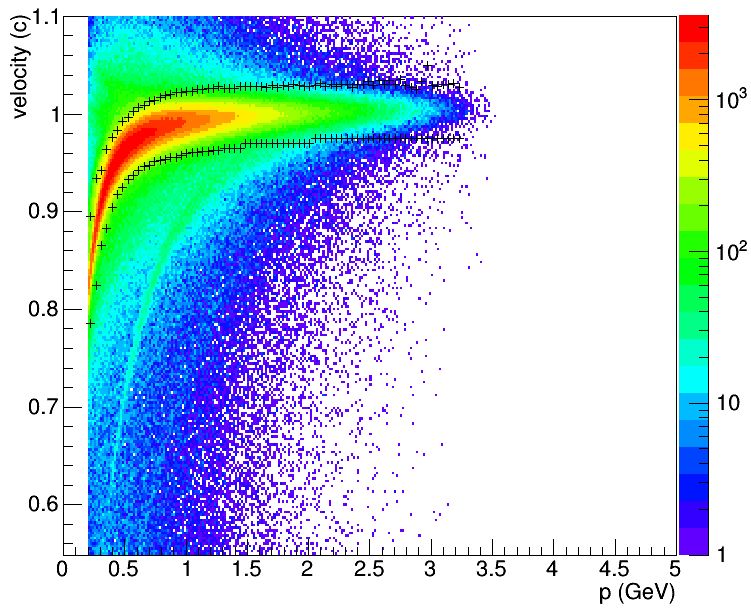
\includegraphics[width=4in]{figures/pim_vvpCut.png}
\caption{The two dimensional view of the $\pi^-$ $\beta$ cut. The black crosses show the upper and lower cut for each of the 70 momentum bins.}
\label{fig:pim_vvpCut}
\end{figure}
%
%
\subsection{$\pi^-$ Fiducial Cut}
To improve the data quality, a geometric fiducial cut is applied to region 1 of the DC.
The cut is shown with red lines in figure~\ref{fig:pim_R1cut_s4}.
The diagonal lines are symmetric and form an $80^\circ$ angle and intersect at $(0, 20)$ cm.
The horizontal line is at X = 24 cm.
\begin{figure}[htp]
\centering
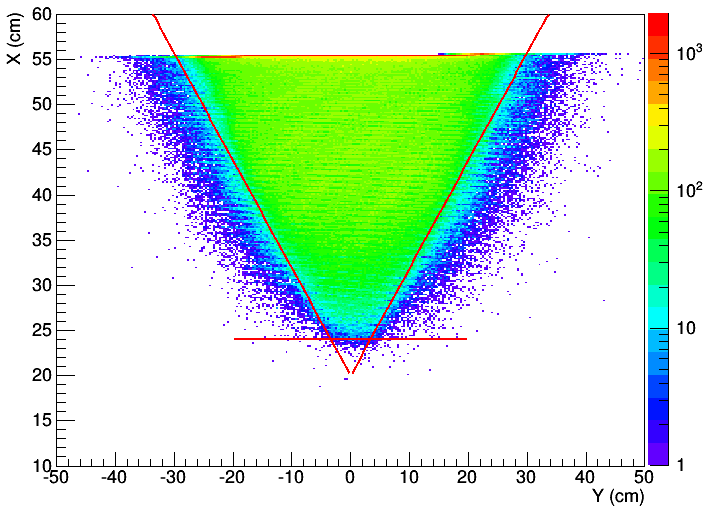
\includegraphics[width=4in]{figures/pim_R1cut_s4.png}
\caption{X vs Y in region 1 of the DC for negative tracks. Events inside of the red lines are kept.}
\label{fig:pim_R1cut_s4}
\end{figure}
%



\chapter{Kinematic Cuts}
\label{cha:KinematicCuts}

\section{SIDIS Cuts}
\label{sec:SIDISCuts}
After identifying particles, kinematic cuts must be implemented to insure the events are within the SIDIS region of phase space.
In order to remove exclusive events as well as events that are not in the deeply inelastic region, the conditions $W > 2.05\ \text{GeV}$ and $Q^2 > 1.0\ \text{GeV}^2$ are imposed.
Traditionally, the $z$ range for SIDIS is $0.4 < z < 0.7$, however, since the results of this analysis are binned in $z$, no cut is applied to $z$ and the entire $z$ range is analyzed.
Note that a missing mass cut has already been applied at the hadron identification stage, as described in chapter~\ref{cha:hadronID}.
%%%%%%%% maybe put a figure here

\section{$\phi_h$ Fiducial Cuts}
\label{sec:phihFiducialCuts}
Certain regions of $x$-$Q^2$-$z$-$P_{h\perp}^2$ space have limited $\phi_h$ coverage (due to acceptance).
The ``holes'' in the $\phi_h$ distribution occur around $\phi_h = 0$ a vast majority of the time.
As the edge of a hole is approached, the number of events begins to drop sharply.
This ``edge effect'' is difficult to describe realistically with simulations (simulations and acceptance studies are discussed in chapter~\ref{cha:MonteCarlo}), therefore a cut is applied to eliminate these regions.

For example, figure~\ref{fig:rec_pip_phih_x3_QQ0_z7_PT21} shows the $\pi^+$ $\phi_h$ distribution for $0.4 < x < 0.5$, $2.2 < Q^2 < 2.8 \text{GeV}^2$, $0.35 < z < 0.4$, and $0.05 < P_{h\perp}^2 < 0.1$.
It can be seen that just inside of $\pm 50^\circ$ the number of events begins to drop off to zero.
In this example, events with $-50^\circ < \phi_h < 50^\circ$ are cut to eliminate the edges.
Every $x$-$Q^2$-$z$-$P_{h\perp}^2$ bin has a different $\phi_h$ fiducial cut (if a cut is necessary) which was determined by eye, placing the cut at the location in $\phi_h$ where the distribution starts dropping off to zero.
%
\begin{figure}[htp]
\centering
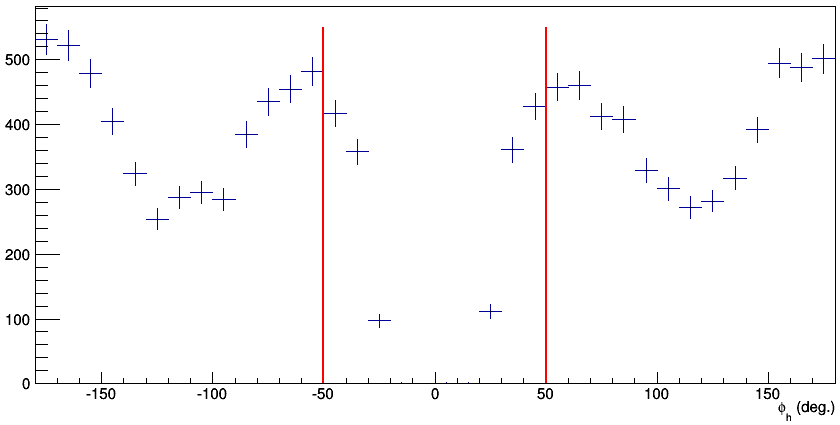
\includegraphics[width=4in]{figures/rec_pip_phih_x3_QQ0_z7_PT21.png}
\caption{The $\pi^+$ $\phi_h$ distribution for $0.4 < x < 0.5$, $2.2 < Q^2 < 2.8 \text{GeV}^2$, $0.35 < z < 0.4$, and $0.05 < P_{h\perp}^2 < 0.1$. The vertical red lines show the $\phi_h$ fiducial cut for this particular bin; events inside of the lines are cut to eliminate edge effects.}
\label{fig:rec_pip_phih_x3_QQ0_z7_PT21}
\end{figure}
%

\section{Elimination of Decay Generated Electrons}
\label{sec:decayGeneratedElectrons}
Dalitz decay of $\pi^0$s ($\pi^0 \rightarrow \gamma e^+ e^-$) and pair production from photons can produce electron-positron pairs.
These decay generated electrons are a possible cause of contamination in the electron sample, however, Monte Carlo studies using PYTHIA and PEPSI indicate that the $y$ values for these electrons tend to be large.
The cut removing events with $y > 0.8$ should therefore eliminate all but a negligible number of decay generated electrons.
This result can be seen in figure~\ref{fig:decayElectronRemoval} and is also consistent with a similar study in \cite{Prok14}.
%
\begin{figure}[htp]
\centering
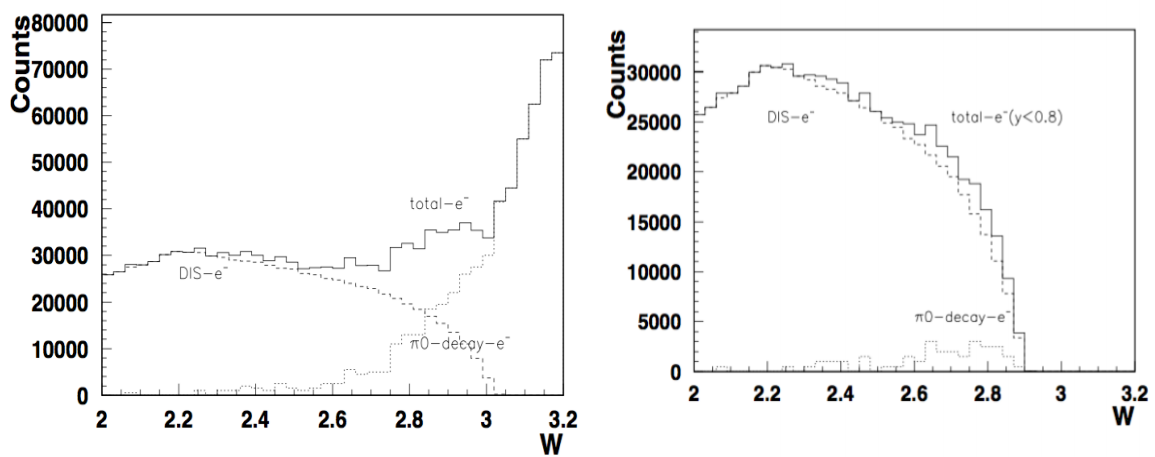
\includegraphics[width=6in]{figures/decayElectronRemoval.png}
\caption{W distributions for DIS electrons (dashed line) and decay generated electrons (dotted line) without a $y$ cut (left) and with a $y<0.8$ requirement (right). The $y$ cut removes nearly all of the decay generated electrons.}
\label{fig:decayElectronRemoval}
\end{figure}

\chapter{Momentum Corrections}
\label{cha:MoCo}
%
The CLAS detector may have some small misalignments and imperfections in the magnetic field that can cause a particle's reconstructed momentum to be slightly off.
This effect can be corrected by studying well known processes, such as elastic events ($ep \rightarrow ep$), Bethe-Heitler events ($ep \rightarrow ep\gamma$), and exclusive events such as $ep \rightarrow e\pi^+n$.
%%%The correction functions used for this analysis were developed by Marco Mirazita \cite{MirazitaMoCo}.
A set of correction functions were determined in order to shift the kinematics of these events to their proper values \cite{MirazitaMoCo}.
The following section show results with and without the corrections to demonstrate their efficacy.
%
\section{Electron Momentum Corrections}
\label{sec:eMoCo}
%
A first step in checking the efficacy of electron momentum corrections is to look at the missing mass distribution of $ep \rightarrow eX$ events near the proton mass, which are elastic events (missing mass is the same as $W$ in this context).
As seen in figures~\ref{fig:W_eX_without} and~\ref{fig:W_eX_with}, the momentum corrections produce an improvement in the mean value (bringing it closer to the proton mass) and in the width (making it narrower) of the elastic peak.
When $W$ is plotted as a function of $\phi_{e-}^{lab}$, a visible improvement in the symmetry of the distribution is present (see figures~\ref{fig:WVphi_eX_without} and~\ref{fig:WVphi_eX_with}).
%
\begin{sidewaysfigure}[htp]
\centering
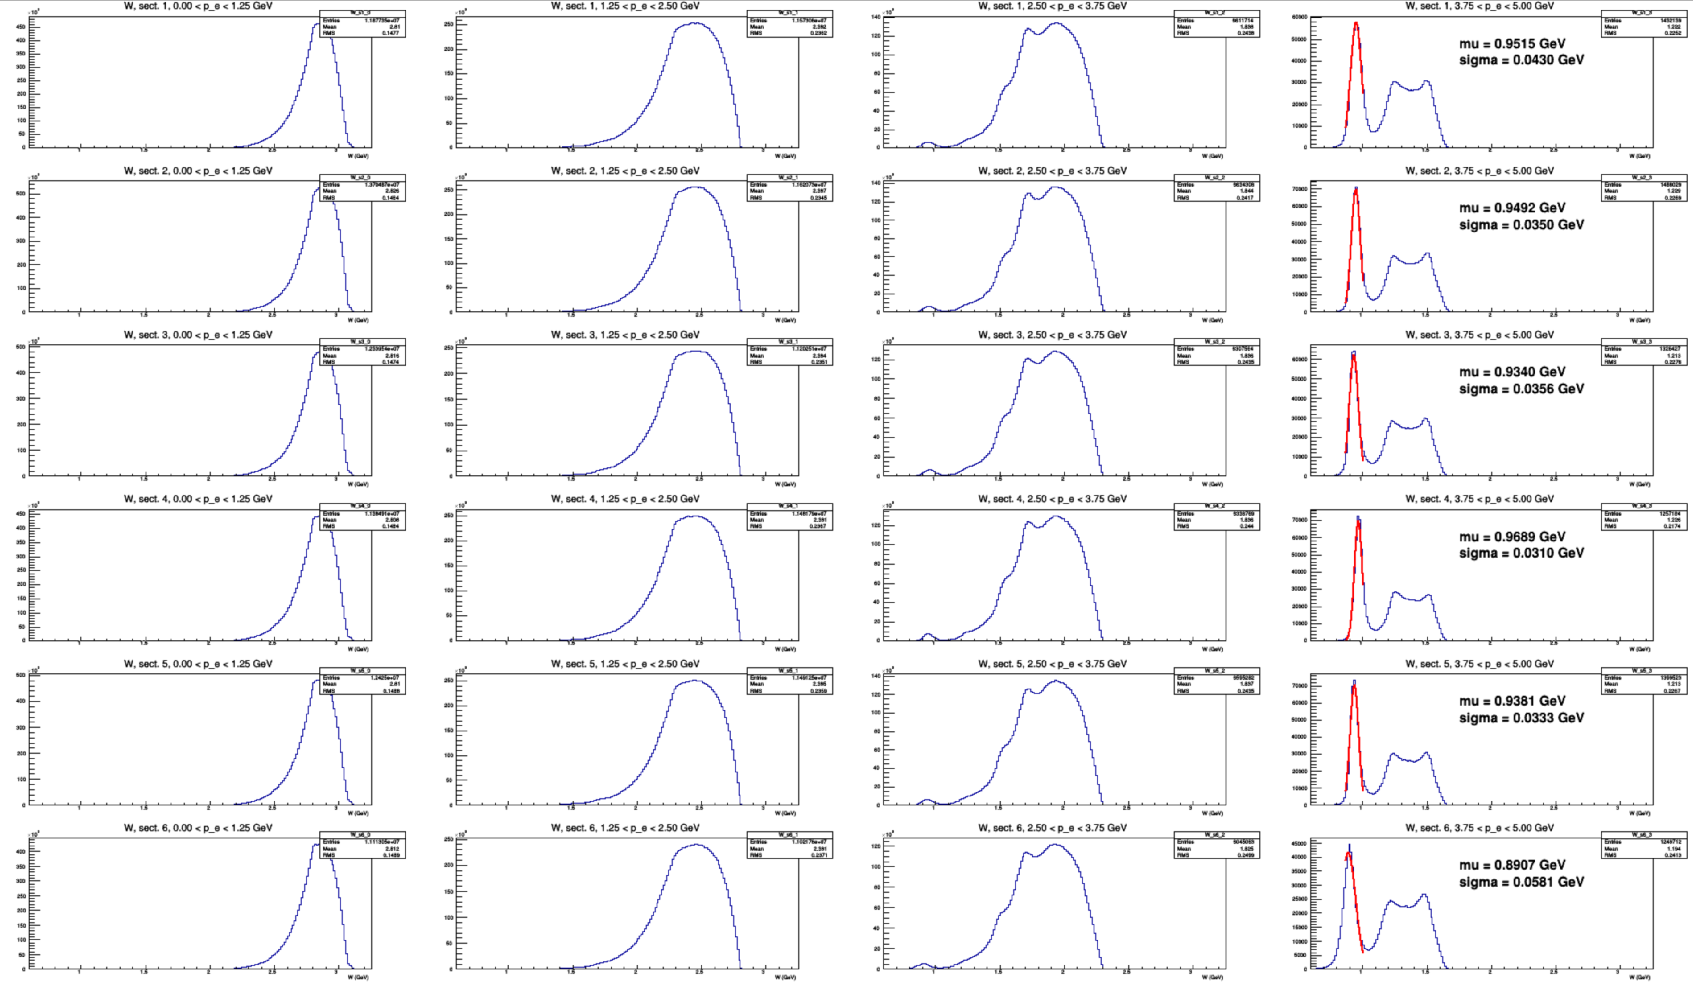
\includegraphics[width=8.5in]{figures/W_eX_without.png}
\caption{Plots of $W$ for $ep \rightarrow eX$ events without momentum corrections. The top row is sector 1, the second row is sector 2, etc. The columns are bins of electron momentum (4 bins from 0 - 5 GeV). The elastic peak becomes visible at higher momenta and is fit with a Gaussian.}
\label{fig:W_eX_without}
\end{sidewaysfigure}
%
\begin{sidewaysfigure}[htp]
\centering
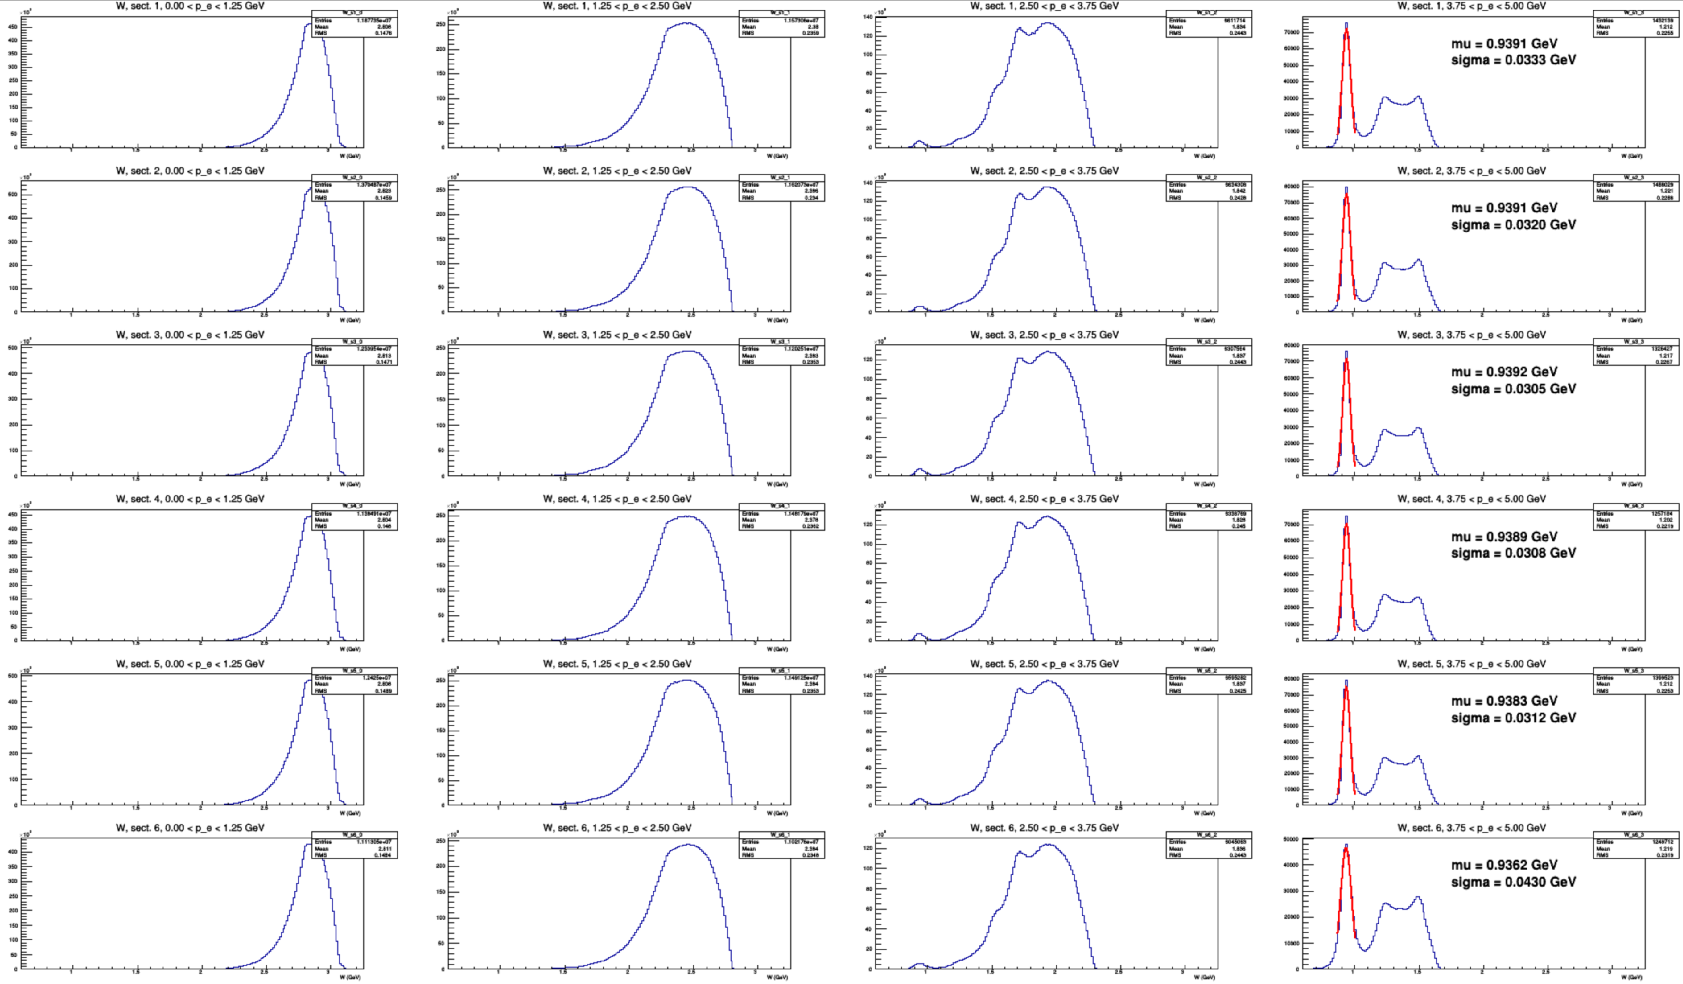
\includegraphics[width=8.5in]{figures/W_eX_with.png}
\caption{The same plots as in figure~\ref{fig:W_eX_without} but with momentum corrections. The mean value (mu) and width (sigma) are both improved for each sector.}
\label{fig:W_eX_with}
\end{sidewaysfigure}
%
\begin{sidewaysfigure}[htp]
\centering
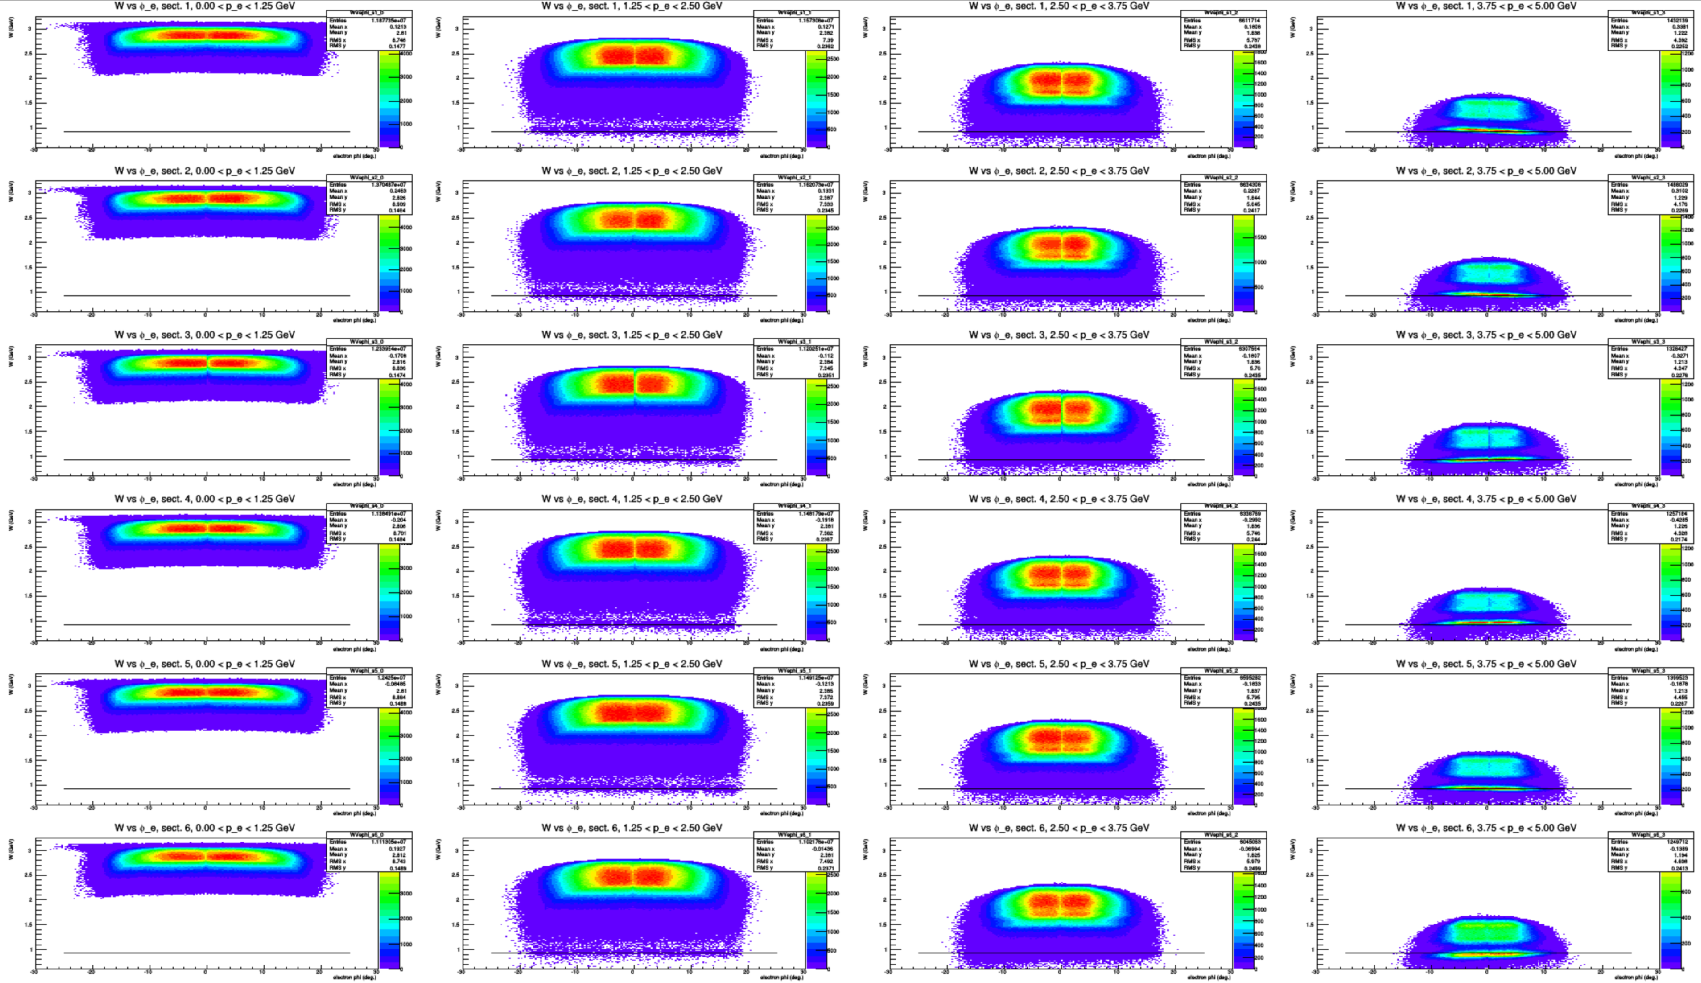
\includegraphics[width=8.5in]{figures/WVphi_eX_without.png}
\caption{Plots of $W$ vs $\phi_{e-}^{lab}$ (relative to the center of the sector) for $ep \rightarrow eX$ events without momentum corrections. The top row is sector 1, the second row is sector 2, etc. The columns are bins of electron momentum (4 bins from 0 - 5 GeV). The elastic peak becomes visible at higher momenta, the black horizontal line shows the location of the proton mass.}
\label{fig:WVphi_eX_without}
\end{sidewaysfigure}
%
\begin{sidewaysfigure}[htp]
\centering
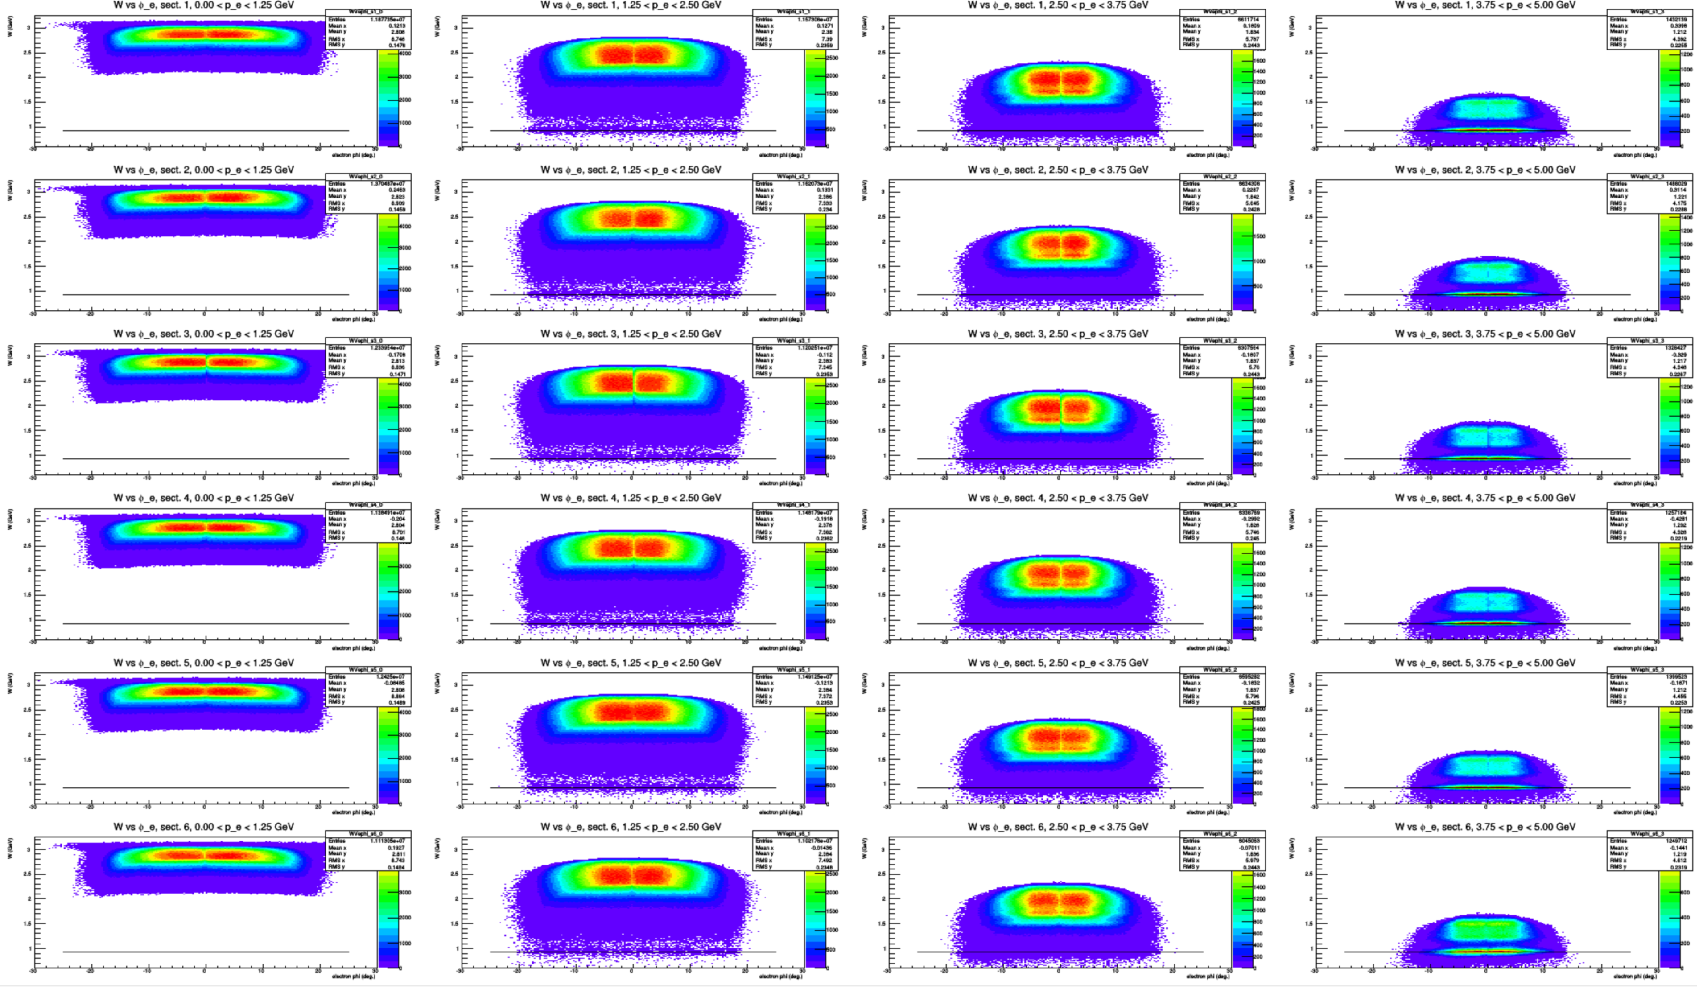
\includegraphics[width=8.5in]{figures/WVphi_eX_with.png}
\caption{The same plots as in figure~\ref{fig:WVphi_eX_without} but with momentum corrections. The symmetry of the distribution is improved for each sector.}
\label{fig:WVphi_eX_with}
\end{sidewaysfigure}

Although the momentum corrections produce an improvement in the $W$ distributions of elastic events, the overlap in phase space coverage between elastic events and SIDIS events is small.
In order to have greater confidence in the momentum corrections, a process with a phase space coverage similar to that of SIDIS events must be studied.
This is done using Bethe-Heitler events.
Bethe-Heitler events are selected using the following criteria: an electron and a proton must be reconstructed, the missing mass squared must be near zero (the photon mass), and the direction of X must be close to either the incoming or outgoing electron direction (since the radiated photon tends to travel in a direction close to that of the electron which radiated it, as shown in figure~\ref{fig:BetheHeitlerDiagrams}).
Since we are looking for events with a phase space coverage similar to that of SIDIS, the additional requirement $W > 2 GeV$ is also added.
%
\begin{figure}[htp]
\centering
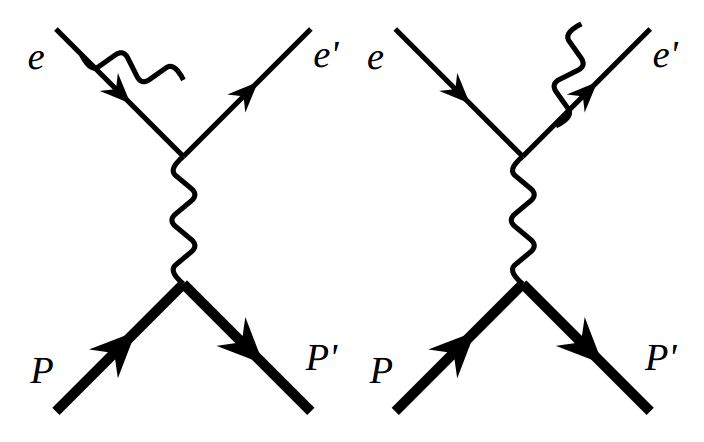
\includegraphics[width=3in]{figures/BetheHeitlerDiagrams.png}
\caption{Left: Pre-radiated Bethe-Heitler process. Right: Post-radiative Bethe-Heitler process. The radiated photon tends to travel in a direction close to that of the electron which radiated it.}
\label{fig:BetheHeitlerDiagrams}
\end{figure}
%

Figure~\ref{fig:h_MX2_eprotX_Wgt2} shows the missing mass squared distribution for $ep \rightarrow epX$ events with $W > 2 GeV$; a cut $-0.05 < M_X^2 < 0.05 GeV^2$ is applied to this quantity to select Bethe-Heitler events.
Furthermore, figure~\ref{fig:eXangles_eprotX_Wgt2} shows the angle between X and the incoming electron ($\Delta\theta_{incoming}$) (left) and the angle between X and the outgoing electron ($\Delta\theta_{outgoing}$) (right) for Bethe-Heitler candidate events.
Events with $\Delta\theta_{incoming} < 0.5$ degrees or $\Delta\theta_{outgoing} < 2$ degrees are kept.
%
\begin{figure}[htp]
\centering
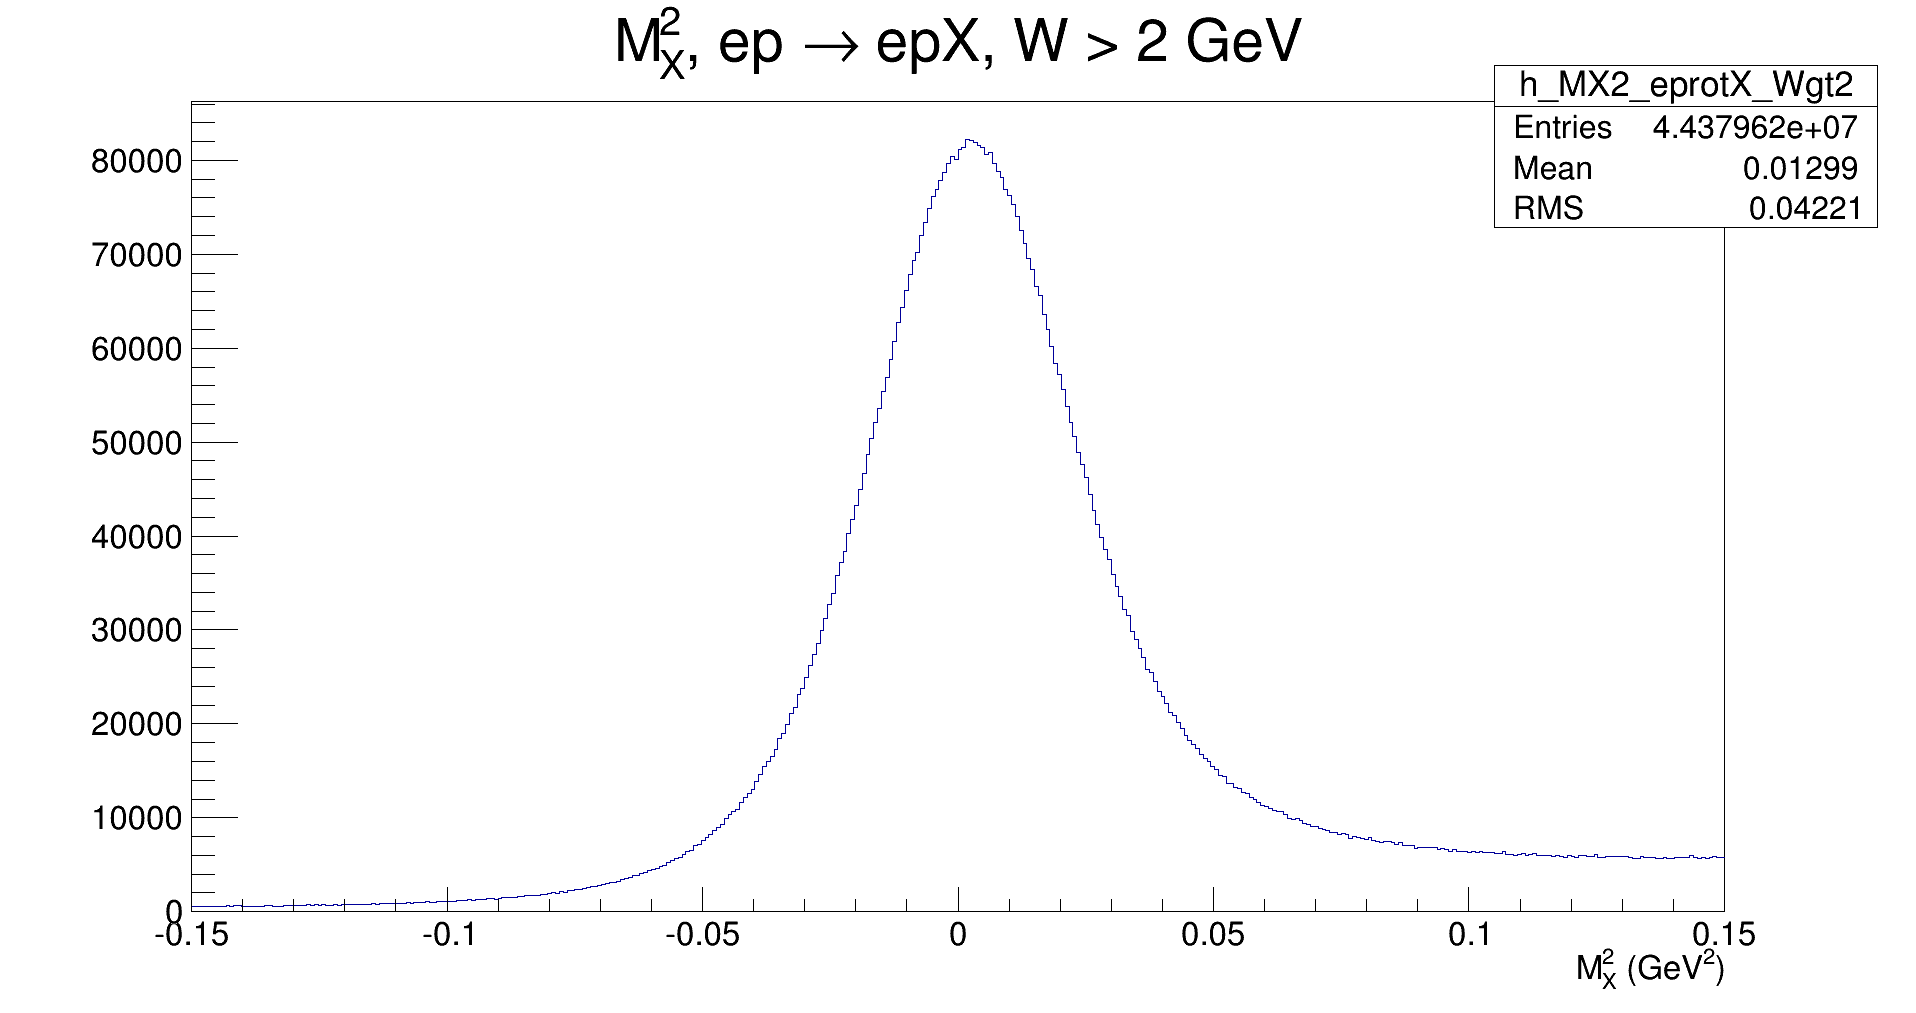
\includegraphics[width=5in]{figures/h_MX2_eprotX_Wgt2.png}
\caption{The missing mass squared distribution for $ep \rightarrow epX$ events with $W > 2 GeV$.}
\label{fig:h_MX2_eprotX_Wgt2}
\end{figure}
%
\begin{figure}[htp]
\centering
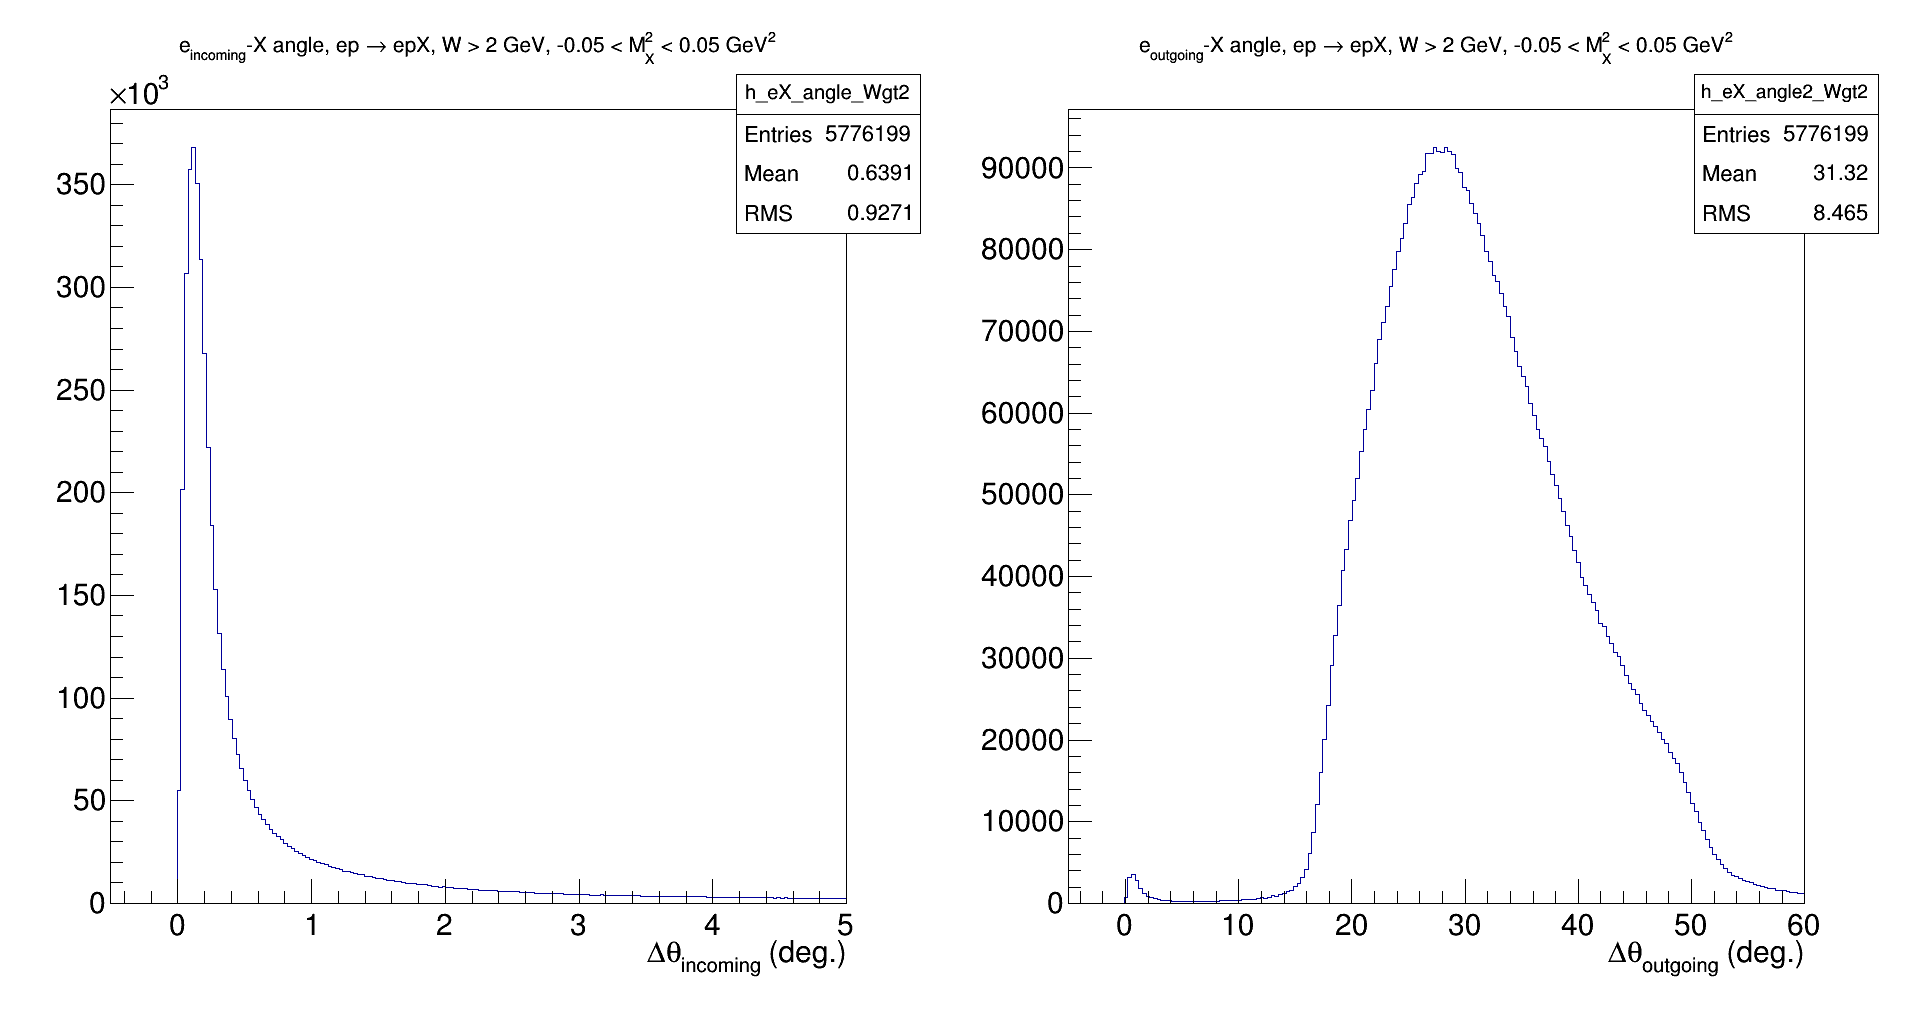
\includegraphics[width=5in]{figures/eXangles_eprotX_Wgt2.png}
\caption{Left: $\Delta\theta_{incoming}$ and right: $\Delta\theta_{outgoing}$ for $ep \rightarrow epX$ events with $W > 2 GeV$ and $-0.05 < M_X^2 < 0.05 GeV^2$.}
\label{fig:eXangles_eprotX_Wgt2}
\end{figure}
%

Returning to the missing mass squared distribution after applying the $\Delta\theta_{incoming}$ and $\Delta\theta_{outgoing}$ cuts (figure~\ref{fig:MX2_BHevents}), it can be seen that the momentum corrections produce a small improvement in the peak position (bringing it closer to zero) while the width does not change significantly.
Likewise, when the missing mass squared is plotted as a function of $\phi_{e-}^{lab}$ (relative to the center of the sector), a visible improvement is noticeable in the symmetry of the distributions after momentum corrections are applied (see figure~\ref{fig:MX2Vphi_BHevents}).
%
\begin{sidewaysfigure}[htp]
\centering
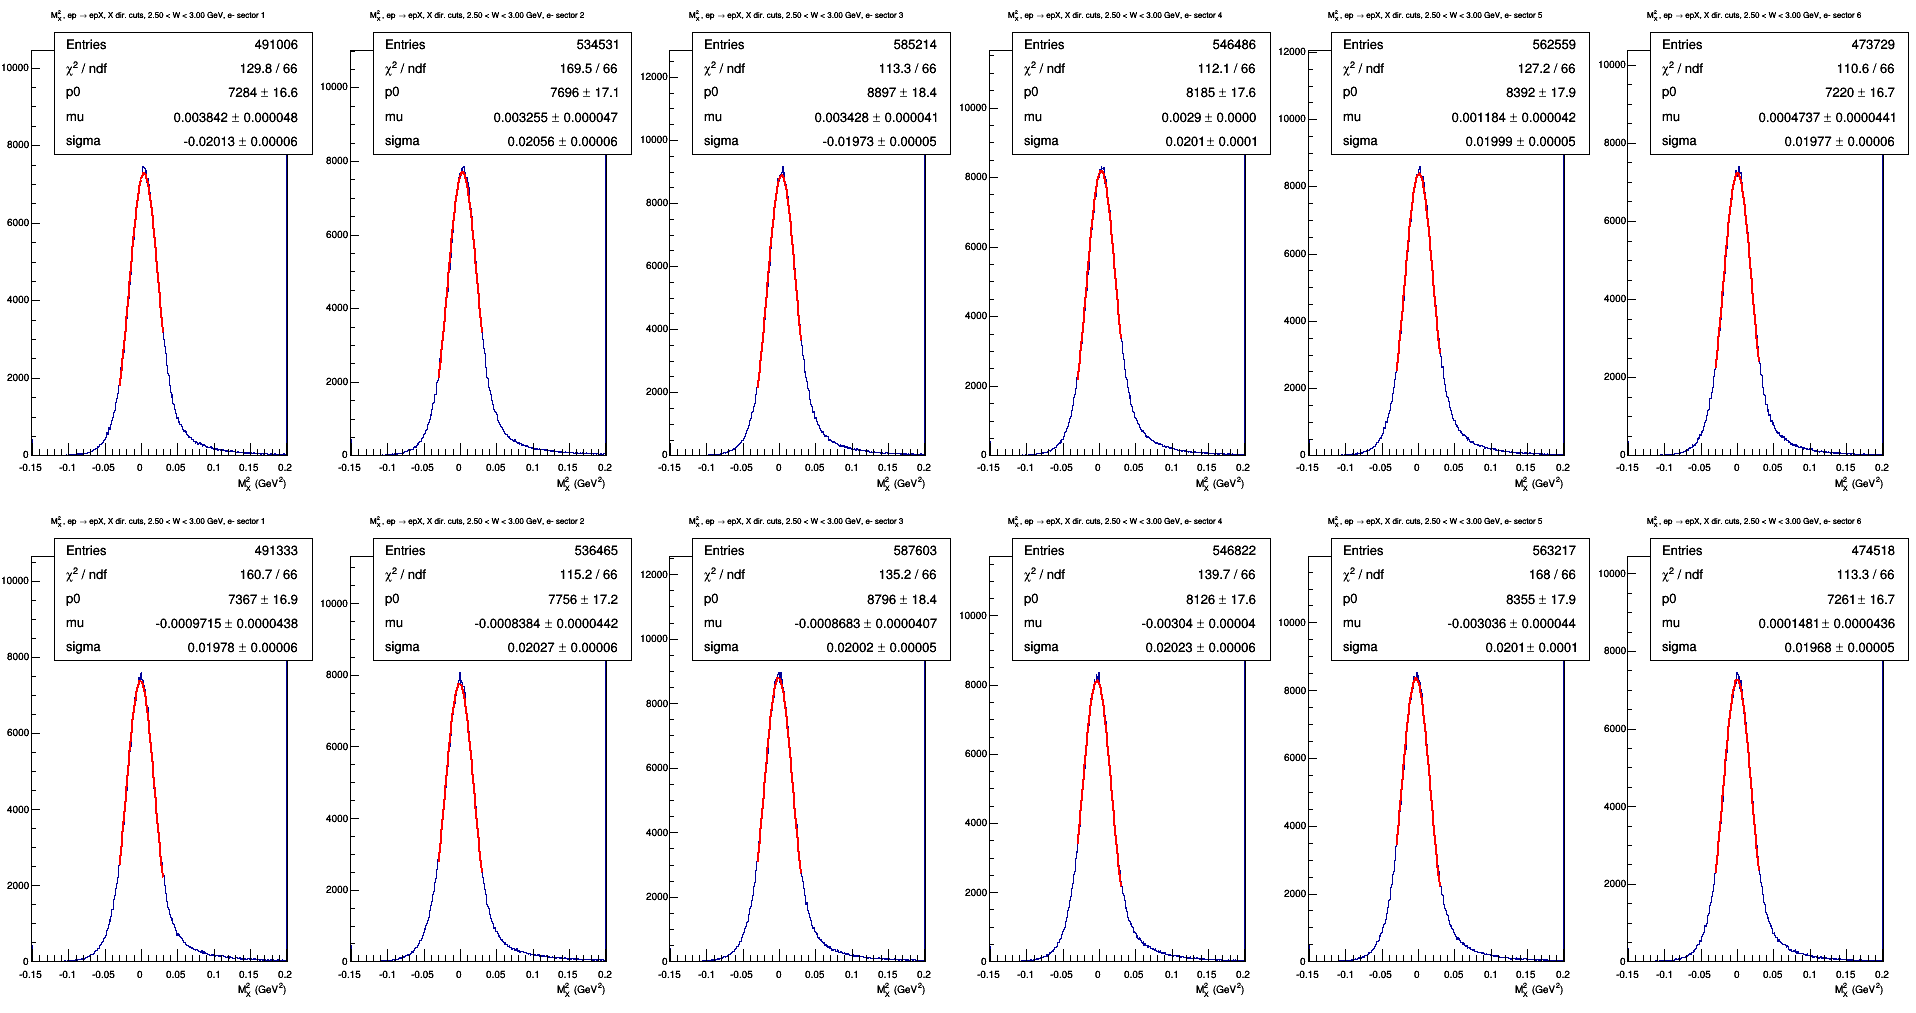
\includegraphics[width=8.5in]{figures/MX2_BHevents.png}
\caption{The missing mass squared distribution for Bethe-Heitler events. The first column is for events with the electron in sector 1, second column sector 2, etc. The top row is without momentum corrections and the bottom row is with the corrections.}
\label{fig:MX2_BHevents}
\end{sidewaysfigure}
%
\begin{sidewaysfigure}[htp]
\centering
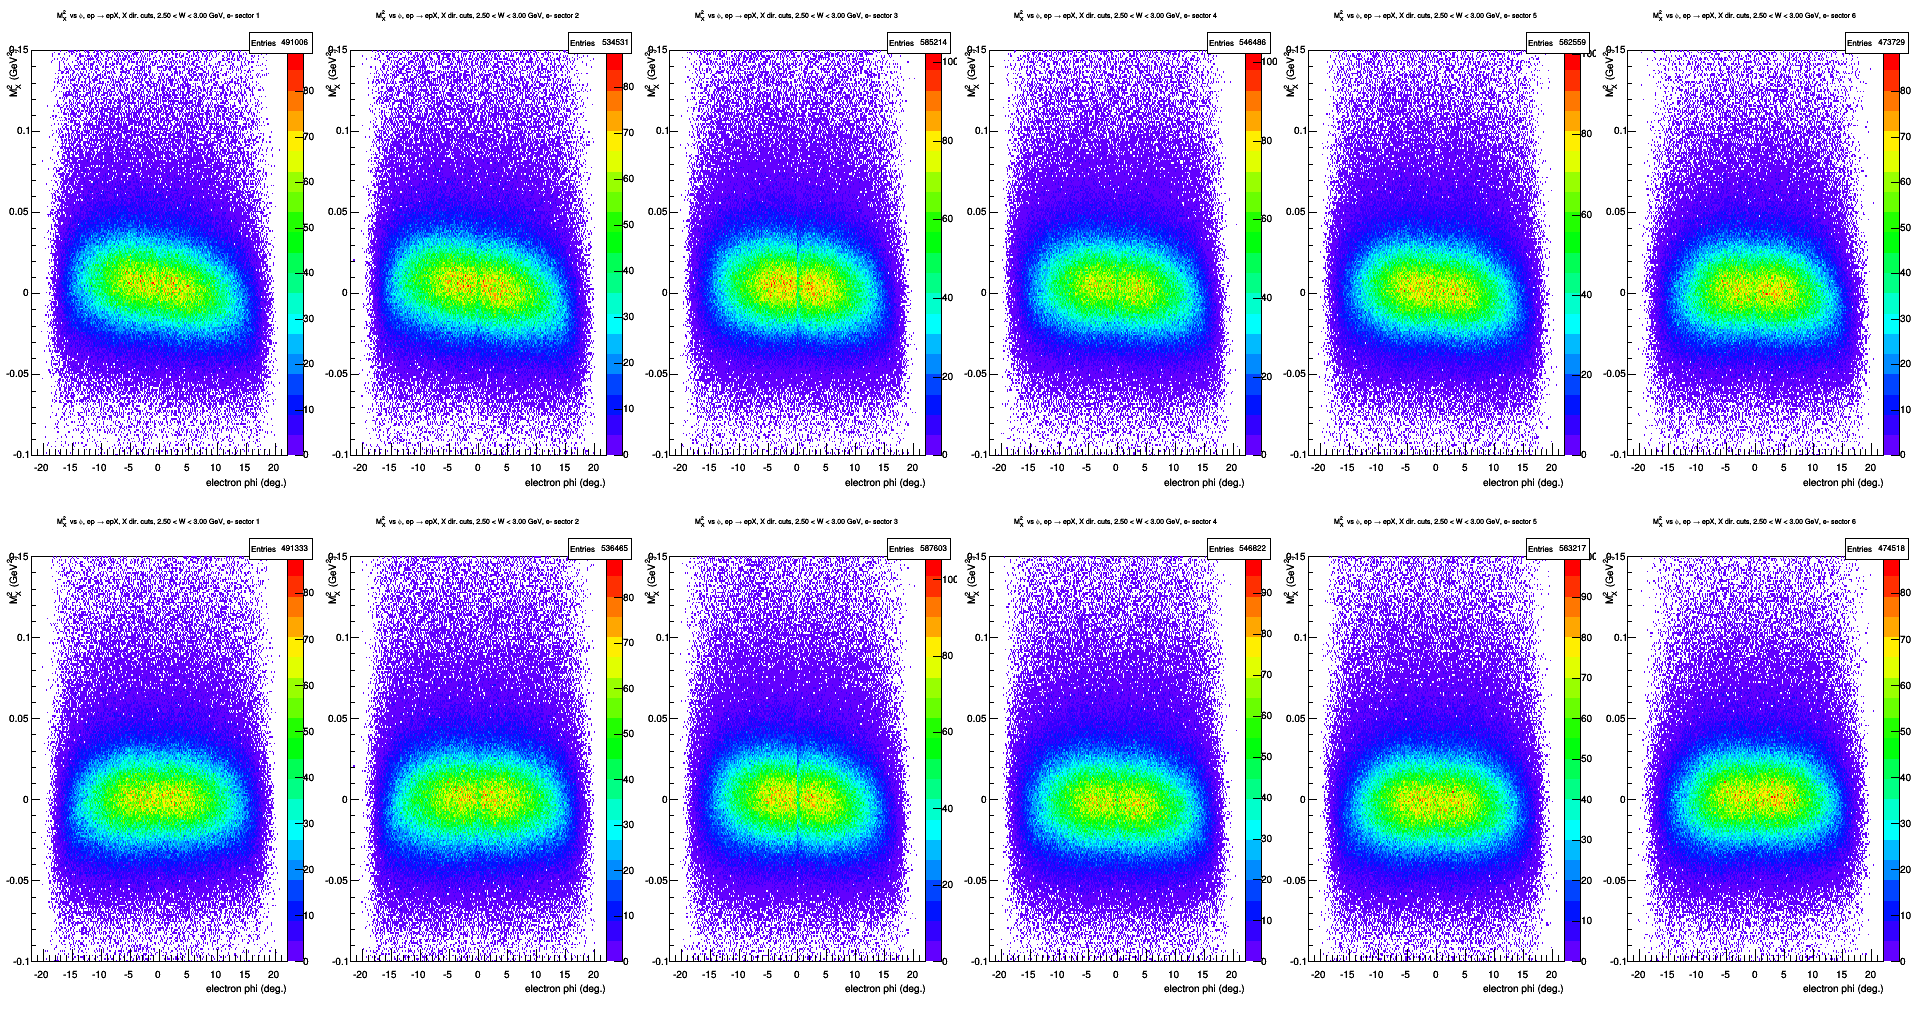
\includegraphics[width=8.5in]{figures/MX2Vphi_BHevents.png}
\caption{The missing mass squared vs $\phi_{e-}^{lab}$ (relative to the center of the sector) distribution for Bethe-Heitler events. The first column is for events with the electron in sector 1, second column sector 2, etc. The top row is without momentum corrections and the bottom row is with the corrections.}
\label{fig:MX2Vphi_BHevents}
\end{sidewaysfigure}
%

The $Q^2-x$ space for Bethe-Heitler events with $W > 2 GeV$ is plotted in figure~\ref{fig:QQVx_BHevents} to confirm that the phase space coverage of these events is similar to that of SIDIS events.
%
\begin{figure}[htp]
\centering
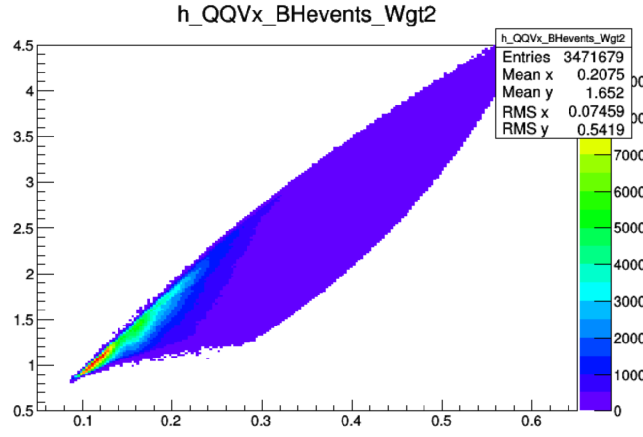
\includegraphics[width=5in]{figures/QQVx_BHevents.png}
\caption{The $Q^2-x$ space for Bethe-Heitler events with $W > 2 GeV$. This coverage is similar to that of SIDIS events which makes Bethe-Heitler events useful for studying momentum corrections in a SIDIS analysis such as this one.}
\label{fig:QQVx_BHevents}
\end{figure}
%

The electron momentum correction functions studied here have been shown to improve the kinematic distributions of well know processes with similar phase space coverage as SIDIS events, making them suitable for this analysis.
Hadron momentum corrections were also applied.
It is worth noting that the effects of these corrections on the final observables are negligible. This can be seen in figures~\ref{fig:compareMoCo_pip} ($\pi^+$ channel) and~\ref{fig:compareMoCo_pim} ($\pi^-$ channel) which show the ratio of $\phi_h$ distributions with and without momentum corrections for several bins of $z$ and $P_{h\perp}^2$.
%
\begin{figure}[htp]
\centering
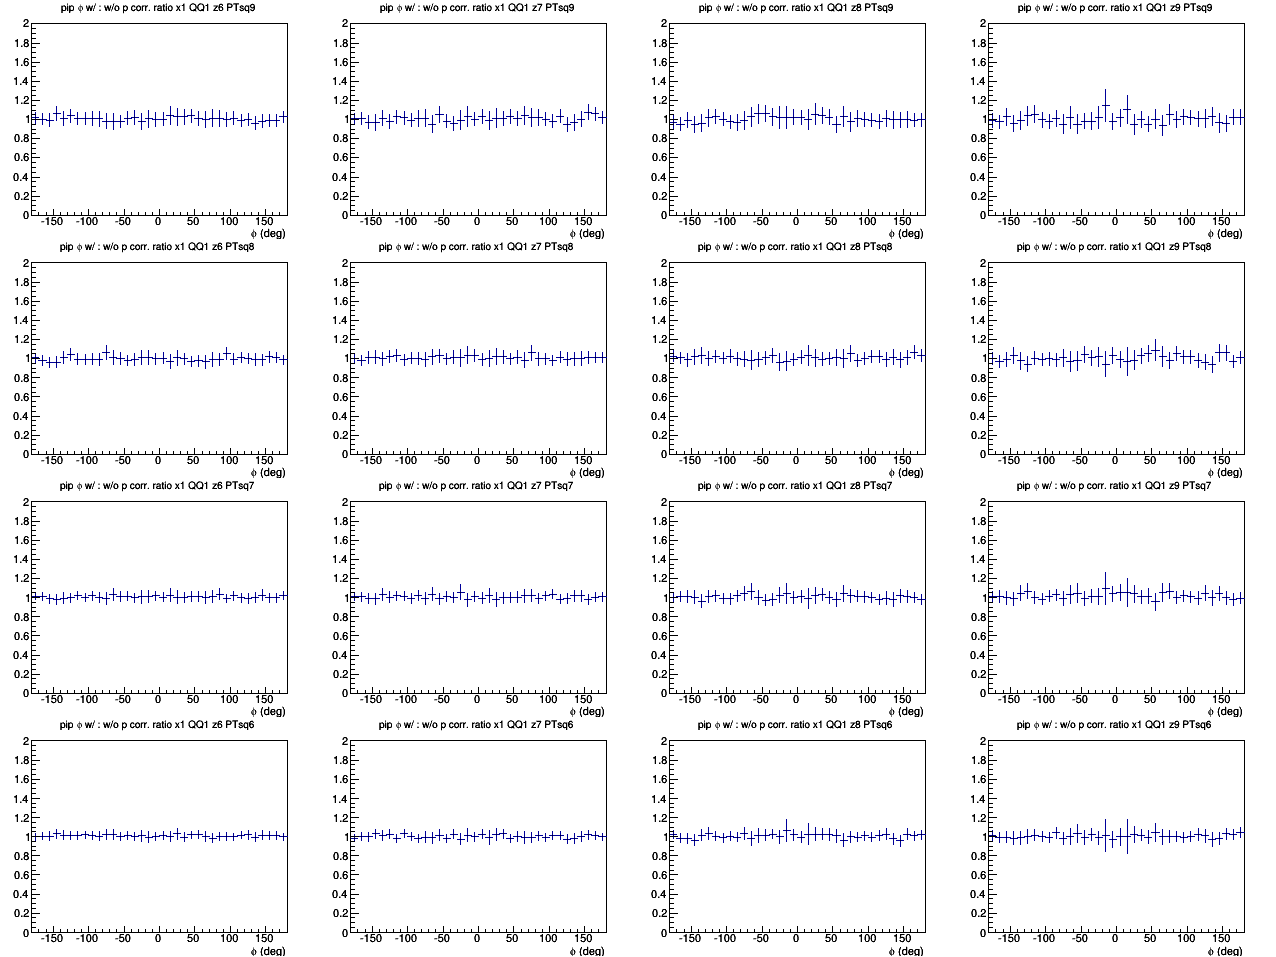
\includegraphics[width=6in]{figures/compareMoCo_pip.png}
\caption{Ratio of $\phi_h$ distributions with and without momentum corrections for the $\pi^+$ channel for several $z$ bins (columns) and $P_{h\perp}^2$ bins (rows).}
\label{fig:compareMoCo_pip}
\end{figure}
%
\begin{figure}[htp]
\centering
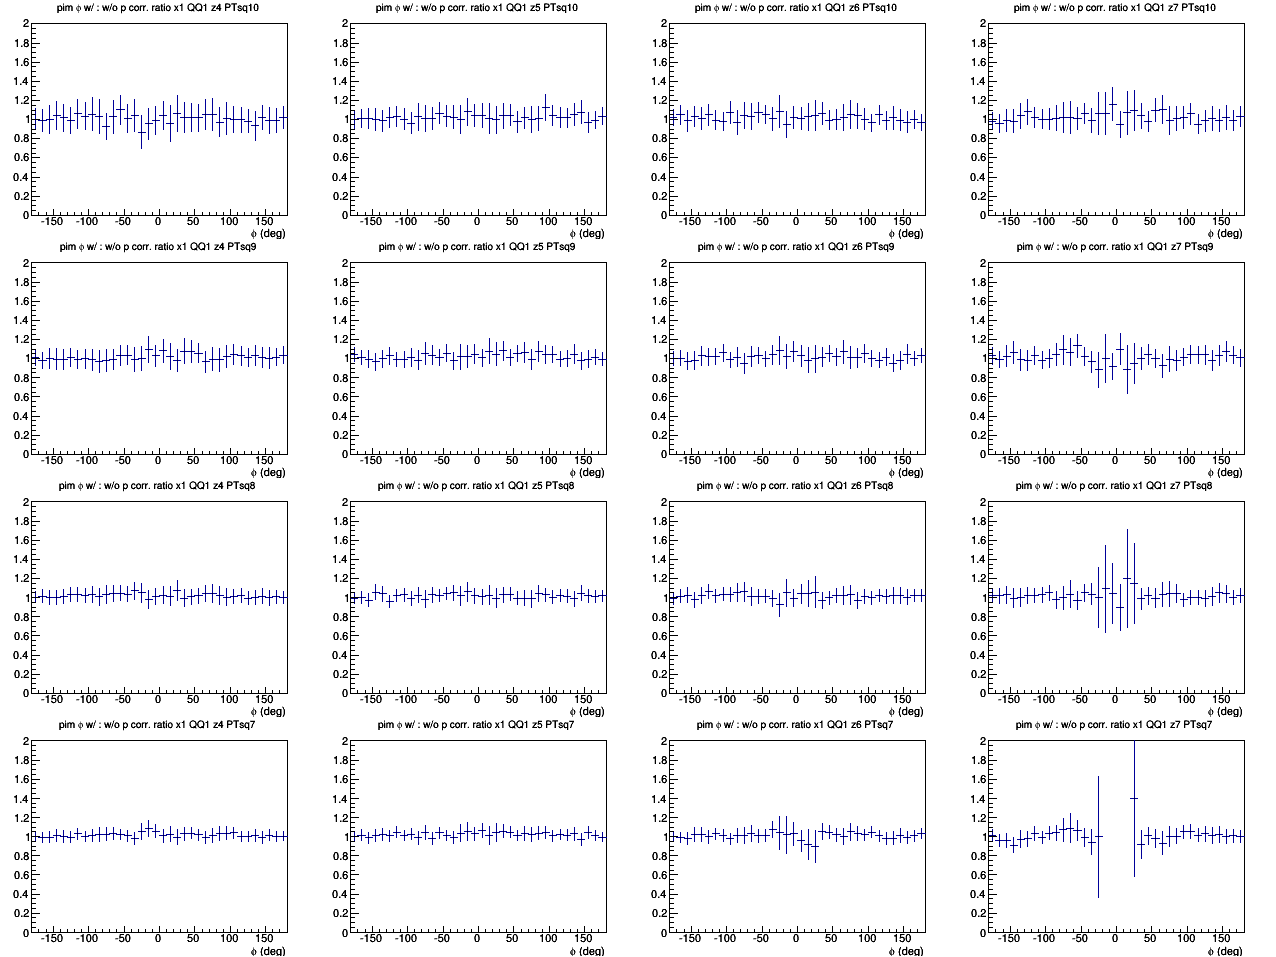
\includegraphics[width=6in]{figures/compareMoCo_pim.png}
\caption{Ratio of $\phi_h$ distributions with and without momentum corrections for the $\pi^-$ channel for several $z$ bins (columns) and $P_{h\perp}^2$ bins (rows).}
\label{fig:compareMoCo_pim}
\end{figure}
%

\clearpage % should prevent a backlog of figures from piling up

\chapter{Monte Carlo Simulations}
\label{cha:MonteCarlo}
%
$\phi_h$ distributions at CLAS are highly dependent on acceptance.
Here, acceptance refers to both geometrical acceptance (the location of active detector elements) and the efficiency in the active regions.
The $cos\phi_h$ and $cos2\phi_h$ moments, therefore, cannot be extracted without acceptance corrections.
This is done using Monte Carlo simulations.
An event generator is used to create a realistic large set of events (several iterations may be required before the set is ``realistic'') which are passed through a GEANT based simulation of the CLAS detector.
For a given kinematic space, the acceptance is equal to the number of reconstructed events divided by the number of generated events.
The number of events in the E1-f data is then divided by the acceptance to get a corrected value for the number of events.
%
\section{Simulation}
\label{sec:Simulation}
%
Below is a general outline for how the simulations are performed.
The details for each step will be discussed in the subsequent subsections.
\begin{itemize}
\item clasDIS is a program that generates electron-proton scattering events.
\item GSim is a program that attempts recreate how CLAS would reconstruct the generated events.
\item GPP (GSim Post Processing) is a program that smears and introduces additional inefficiencies to the GSim results to make the resolutions and acceptance more realistic.
\item the RECSIS software cooks and formats the raw data using the same procedure as in the E1-f cooking and formatting.
\item the same particle ID and fiducial cuts used in the E1-f data are used on the simulation.
\end{itemize}
%
\subsection{Event Generation}
\label{subsec:EventGeneration}
%
The first step in doing Monte Carlo simulations is event generation.
The distribution of events created by the generator should resemble nature as closely as possible.
Since the $cos\phi_h$ and $cos2\phi_h$ moments are not known a priori, this is accomplished in an iterative way, starting with a flat $\phi_h$ distribution (i.e. $A^{cos\phi_h}_{UU} = A^{cos2\phi_h}_{UU} = 0$).
The program used to do this is clasDIS, which is based on the PYTHIA generator and has been modified to be compatible with the kinematics at CLAS.
The control options used with clasDIS for this analysis are summarized in table~\ref{tab:clasDIScontrolOpts}.
Approximately one billion events were generated in order to minimize the statistical error of the acceptance calculations.
%
\begin{table}[htp]
\centering
\begin{tabular}{ p{4cm} p{10cm} }
\hline
\textbf{Option} & \textbf{Description} \\ \hline
--trig N & Tells the generator to process N events. \\
--datf & Tells the generator to output a data file. \\
--outform 2 & Tells the generator to format the output for GSim. \\
--beam 5498 & Sets the beam energy to 5.498 GeV. \\
--zpos -250 & Sets the z-position at -250 mm. \\
--zwidth 25 & Sets the target half-width to 25 mm. \\
--t 5 60 & Sets the range of acceptable $\theta$ in degrees. \\
--parl3 0.7 & Sets the mean of the $k_T$ distribution, which is tuned such that the output $P_{h\perp}$ matches E1-f. \\
--lst15 145 & Defines the set of parton distribution functions used in the simulation. \\
--parj33 0.3 & Defines the remaining energy below which the fragmentation of a parton system is stopped and two hadrons are formed. \\
\hline
\end{tabular}
\caption{Control options for the clasDIS event generator.}
\label{tab:clasDIScontrolOpts}
\end{table}
%
\subsection{Detector Simulation}
\label{subsec:DetectorSimulation}
%
The software package used to simulate the CLAS detector is GSim.
GSim is a GEANT based Monte Carlo simulation that simulates the passage of particles through matter.
The functionality includes detector geometry, physics models, and particle tracking and hits.
Each event generated with clasDIS is passed to GSim; GSim then produces a realistic reconstruction of how the CLAS detector would reconstruct those events.
Figure~\ref{fig:gsim_int_5events} shows an example of this.
Both the generated information and the reconstructed information of the event are saved in the GSim output data file, the reconstructed portion being identical in format to the E1-f raw data files.

Each experimental run at Jefferson Lab uses slightly different conditions (magnetic field strength, target type/polarization, etc.).
To customize GSim to be compatible with a particular run, a file called ffread.in must included in the GSim options.
The ffread.in file for the E1-f run is summarized in table~\ref{tab:ffread_table}
%
\begin{figure}[htp]
\centering
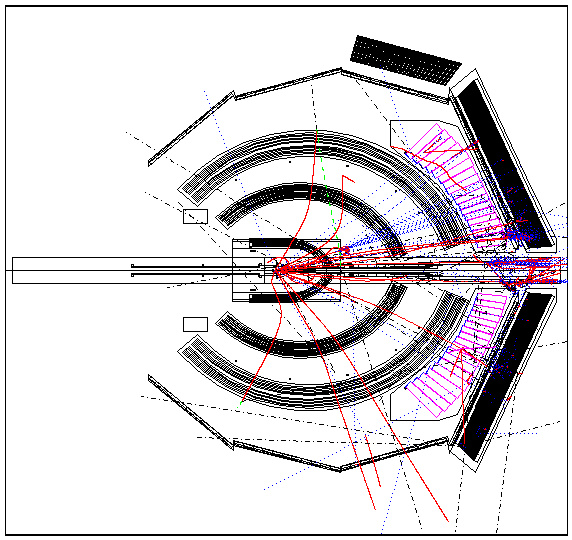
\includegraphics[width=4in]{figures/gsim_int_5events.png}
\caption{A GSim reconstruction of five simulated events. The red tracks represent charged particles while gray tracks represent neutral particles.}
\label{fig:gsim_int_5events}
\end{figure}

\begin{center}
\begin{longtable}{l l}
\caption{The information contained in the ffread.in file, customized for the E1-f run.}\\
\hline
\textbf{Input} & \textbf{Description} \\
\hline
\endfirsthead
\multicolumn{2}{c}%
{\tablename\ \thetable\ -- \textit{Continued from previous page}} \\
\hline
\textbf{Input} & \textbf{Description} \\
\hline
\endhead
\hline \multicolumn{2}{r}{\textit{Continued on next page}} \\
\endfoot
\hline
\endlastfoot
GEOM \lq ALL\rq & Includes all CLAS geometry. \\
NOGEOM \lq PTG\rq \lq ST\rq \lq IC\rq & Excludes geometry not present in E1-f. \\
MAGTYPE 3 & \parbox[t]{7cm}{Sets magnetic field type to ``torus + mini from lookup table.''} \\ %parbox prevents the long sentence from running off the edge of the page
CUTS 5.e-3 5.e-3 5.e-3 5.e-3 & Kinetic energy cuts in GeV. \\
CCCUTS 1.e-3 1.e-3 1.e-3 1.e-3 & Cuts for the \v{C}erenkov counter. \\
DCCUTS 1.e-4 1.e-4 1.e-4 1.e-4 & Cuts for the drift chamber. \\
ECCUTS 1.e-4 1.e-4 1.e-4 1.e-4 & Cuts for the electromagnetic calorimeter. \\
SCCUTS 1.e-4 1.e-4 1.e-4 1.e-4 & Cuts for the time-of-flight detector. \\
NTARGET 2 & Sets the target type to liquid hydrogen. \\
MAGSCALE 0.5829 0.7495 & Sets the scale of the magnetic fields. \\
RUNG 10 & Default setting. \\
TARGET \lq e1e\rq & \parbox[t]{7cm}{Defines the target geometry (e1e is compatible with e1f).} \\
TGMATE \lq PROT\rq \lq ALU\rq & Sets the target and target cell materials. \\
TGPOS 0.00 0.00 -25.0 & Defines the target position. \\
NOMCDATA \lq ALL\rq & \parbox[t]{7cm}{Default setting to turn off additional GEANT hit information.} \\
SAVE \lq ALL\rq \lq LEVL\rq 10 & Save all secondaries up to cascade level 10. \\
KINE 5 & Setting for LUND event generator. \\
AUTO 1 & \parbox[t]{7cm}{Automatic computation of the tracking medium parameters.} \\
STOP & GEANT command to end the ffread file.
\label{tab:ffread_table}
\end{longtable}
\end{center}
%
\subsection{Resolution Matching}
\label{subsec:ResolutionMatching}
%
Since GSim significantly over estimates the detector resolution, the GPP program is used to smear the DC and TOF values.
To determine the amount of DC smearing necessary, studies were done using the reaction $ep \rightarrow e\pi^+ \pi^- p$ in the experimental data and in the Monte Carlo.
These events were selected using the same $e$, $\pi^+$, and $\pi^-$ identification previously described; protons were identified using a momentum dependent $\beta$ cut similar to the pion ID cuts.
Furthermore, a missing mass cut for $e \pi^+ \pi^- p X$ was applied around zero.
After selecting these events, the following resolutions are defined
%
\begin{equation}
\label{eq:resolutionDefinitions}
\begin{split}
\Delta p_{\pi^+} &= p_{\pi^+, calc} - p_{\pi^+, rec} \\
\Delta \theta_{\pi^+} &= \theta_{\pi^+, calc} - \theta_{\pi^+, rec} \\
\Delta \phi_{\pi^+} &= \phi_{\pi^+, calc} - \phi_{\pi^+, rec} \\
\end{split}
\end{equation}
%
where $p$, $\theta$, and $\phi$ are the momentum, $\theta$, and $\phi$ in the lab frame and the $\pi^+, rec$ subscript refers to the actual reconstructed value of the $\pi^+$ while $\pi^+, calc$ is the value calculated based on the momenta of the other three particle and momentum conservation.
These resolutions can be compared for data and simulation and the simulation can be tuned with GPP until the resolutions match.
This tuning is done with three parameters called ``a'', ``b'', and ``c.''
The optimum values for this analysis were found to be $a = b = c = 2.5$.
Comparison between the data and the Monte Carlo with these parameters can be seen in figures~\ref{fig:DeltapRes_dataAndMC}, \ref{fig:DeltaThetaRes_dataAndMC}, and~\ref{fig:DeltaPhiRes_dataAndMC}.
%
\begin{sidewaysfigure}[htp]
\centering
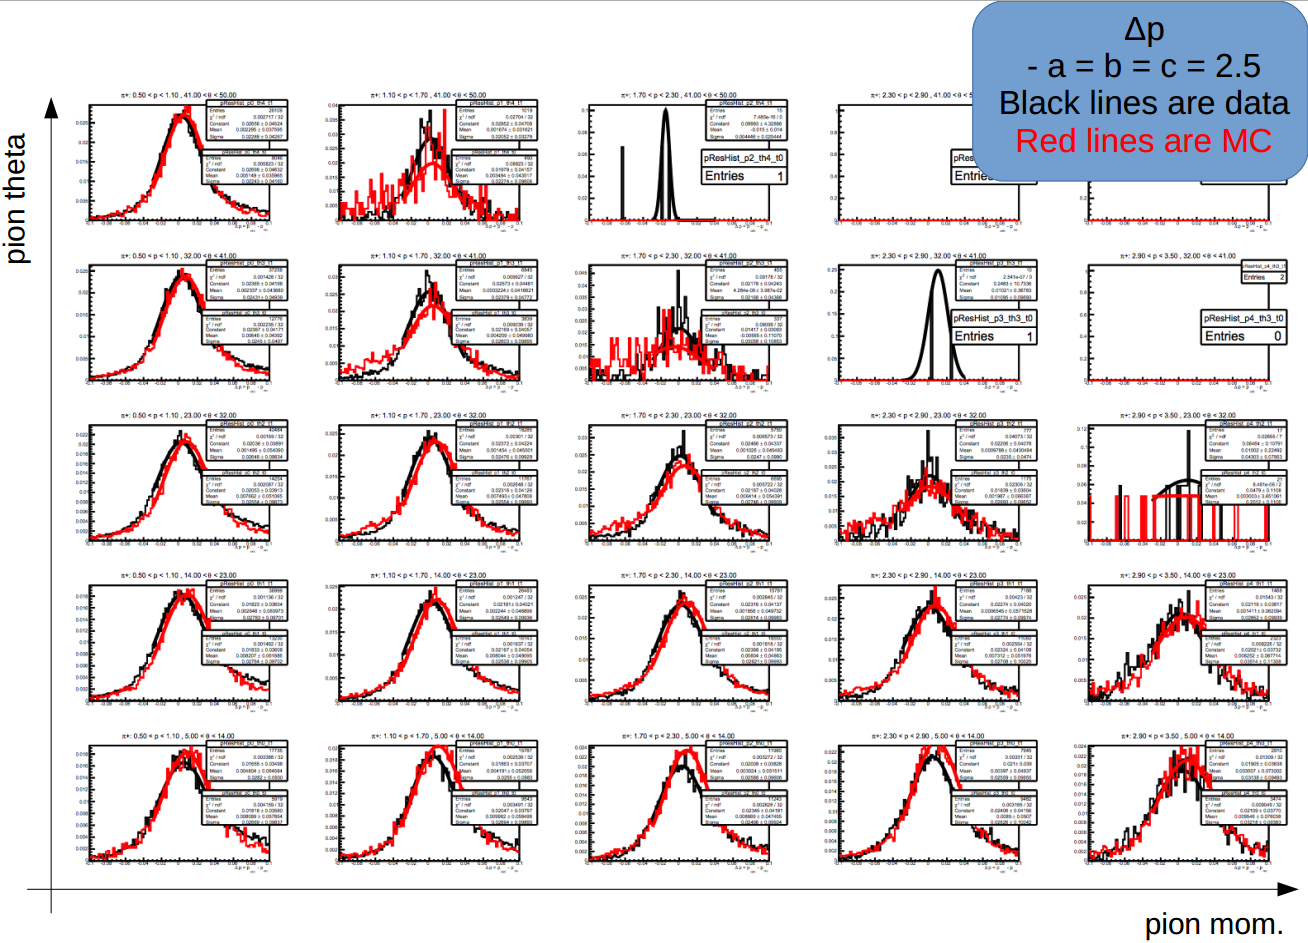
\includegraphics[width=8.5in]{figures/DeltapRes_dataAndMC.png}
\caption{$\Delta p_{\pi^+}$ in bins of $\pi^+$ $\theta$ and $\phi$ for data (black) and Monte Carlo with GPP parameters $a = b = c = 2.5$ (red). It is clear that the agreement in resolution is good between the data and Monte Carlo.}
\label{fig:DeltapRes_dataAndMC}
\end{sidewaysfigure}
%
\begin{sidewaysfigure}[htp]
\centering
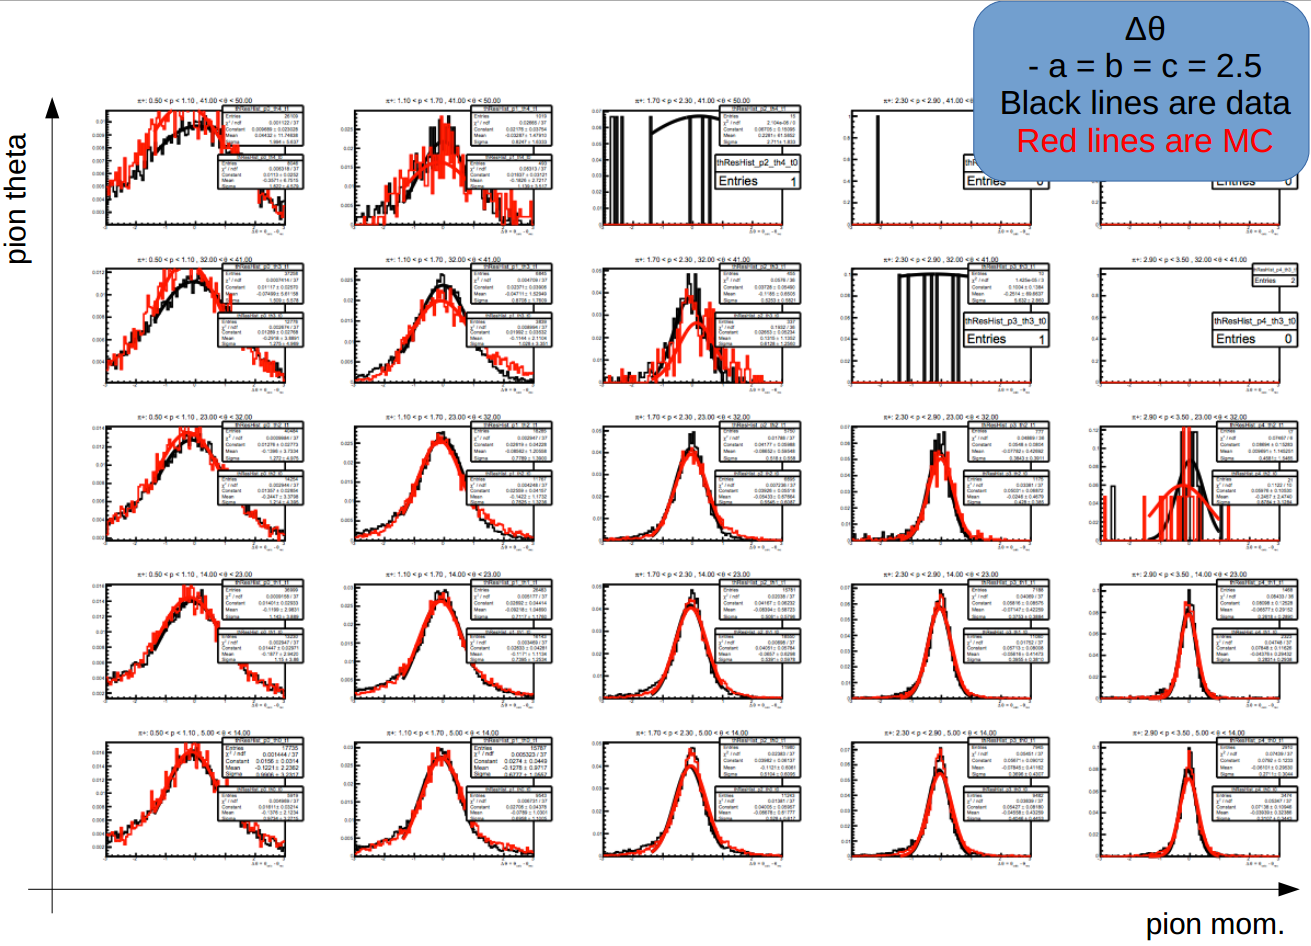
\includegraphics[width=8.5in]{figures/DeltaThetaRes_dataAndMC.png}
\caption{$\Delta \theta_{\pi^+}$ in bins of $\pi^+$ $\theta$ and $\phi$ for data (black) and Monte Carlo with GPP parameters $a = b = c = 2.5$ (red). It is clear that the agreement in resolution is good between the data and Monte Carlo.}
\label{fig:DeltaThetaRes_dataAndMC}
\end{sidewaysfigure}
%
\begin{sidewaysfigure}[htp]
\centering
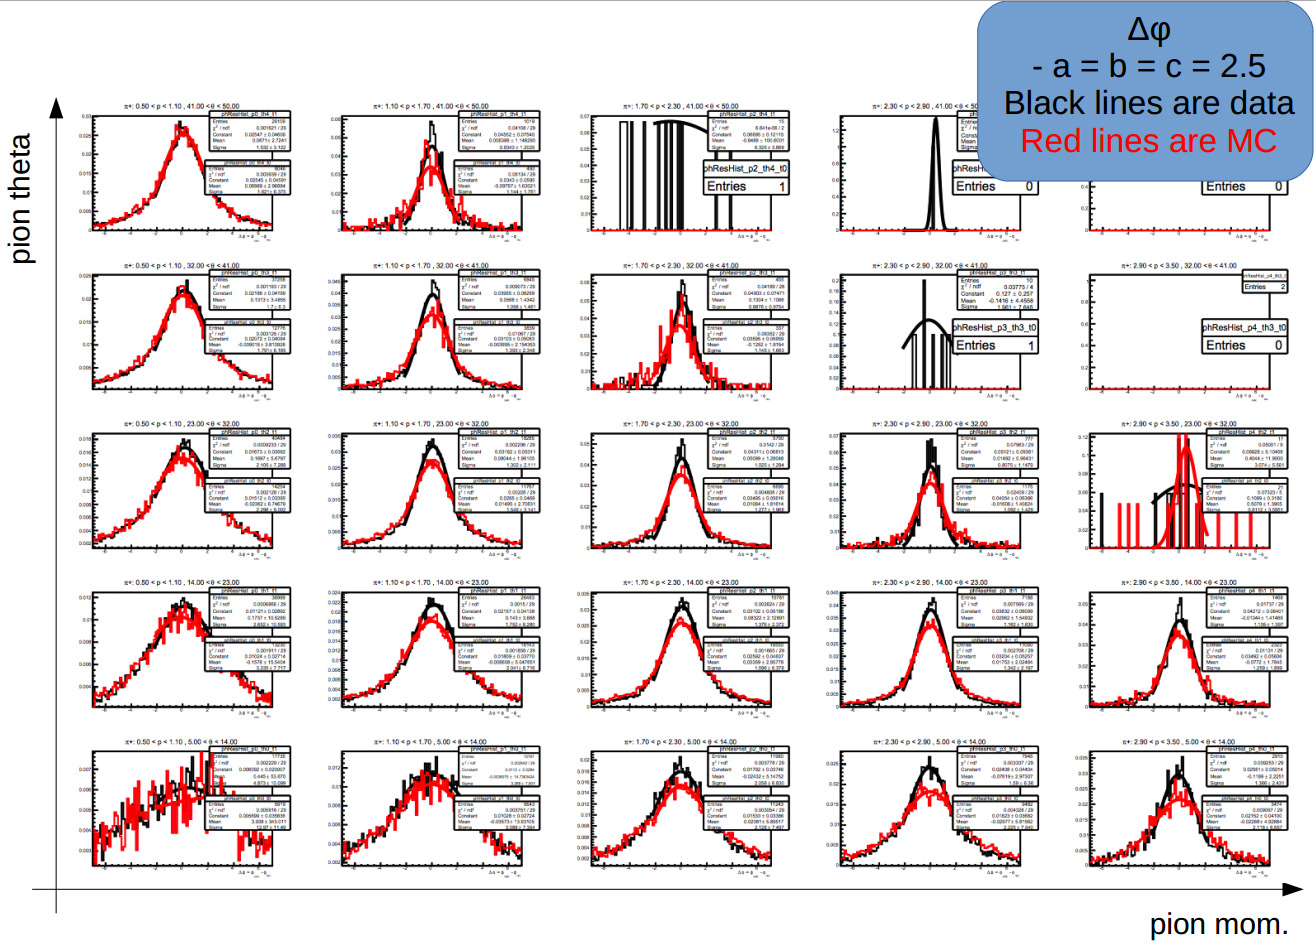
\includegraphics[width=8.5in]{figures/DeltaPhiRes_dataAndMC.png}
\caption{$\Delta \phi_{\pi^+}$ in bins of $\pi^+$ $\theta$ and $\phi$ for data (black) and Monte Carlo with GPP parameters $a = b = c = 2.5$ (red). It is clear that the agreement in resolution is good between the data and Monte Carlo.}
\label{fig:DeltaPhiRes_dataAndMC}
\end{sidewaysfigure}
%

GPP also smears the TOF values via a parameter ``f.''
The f parameter can be tuned by comparing the widths of the $\beta$ distributions (in bins of momentum) for data and Monte Carlo.
It was found that $f = 0.85$ is the best value for this analysis.
Figure~\ref{fig:TOFres_dataAndMC} compares $\pi^+$ $\beta$ for data and Monte Carlo with $f = 0.85$.
%
\begin{sidewaysfigure}[htp]
\centering
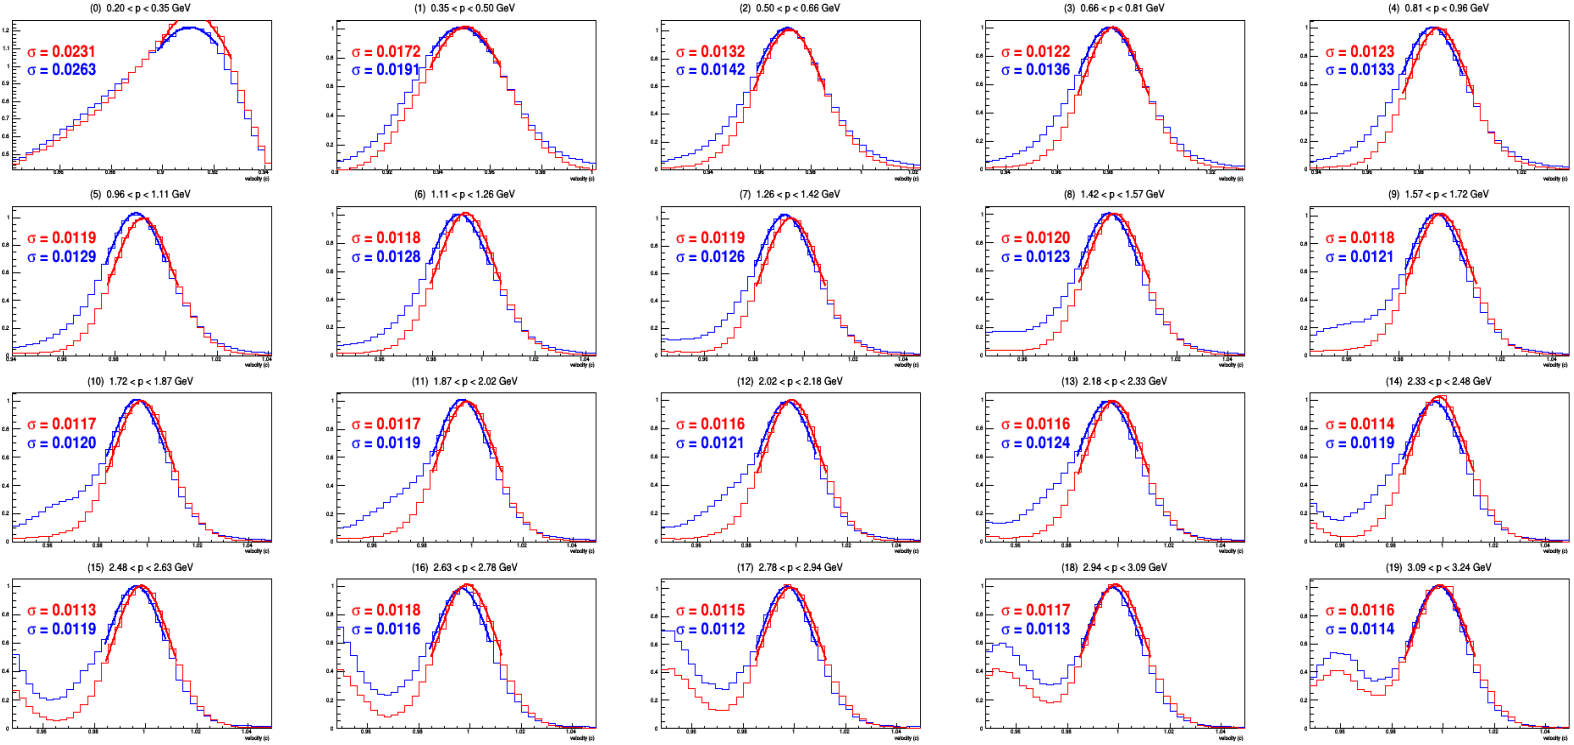
\includegraphics[width=8.5in]{figures/TOFres_dataAndMC.png}
\caption{$\pi^+$ $\beta$ distributions in bins of momentum for data (blue) and Monte Carlo with $f = 0.85$ (red). The top left plot is the lowest momentum bin and the bottom right plot is the highest momentum bin. Each peak is fit with a gaussian and $\sigma$ is printed on the plot (MC on top, data on bottom). This shows the good agreement in TOF resolution between the data and Monte Carlo.}
\label{fig:TOFres_dataAndMC}
\end{sidewaysfigure}
%

The second purpose of GPP is to cut or introduce inefficiencies to certain DC wires in the simulation so that it matches the data.
To check that this worked properly a wire map of the DC occupancy is made for the data and simulation (after using GPP).
This is shown in figure~\ref{fig:DCoccupancy} which confirms the efficacy of this feature of GPP.
%
\begin{sidewaysfigure}[htp]
\centering
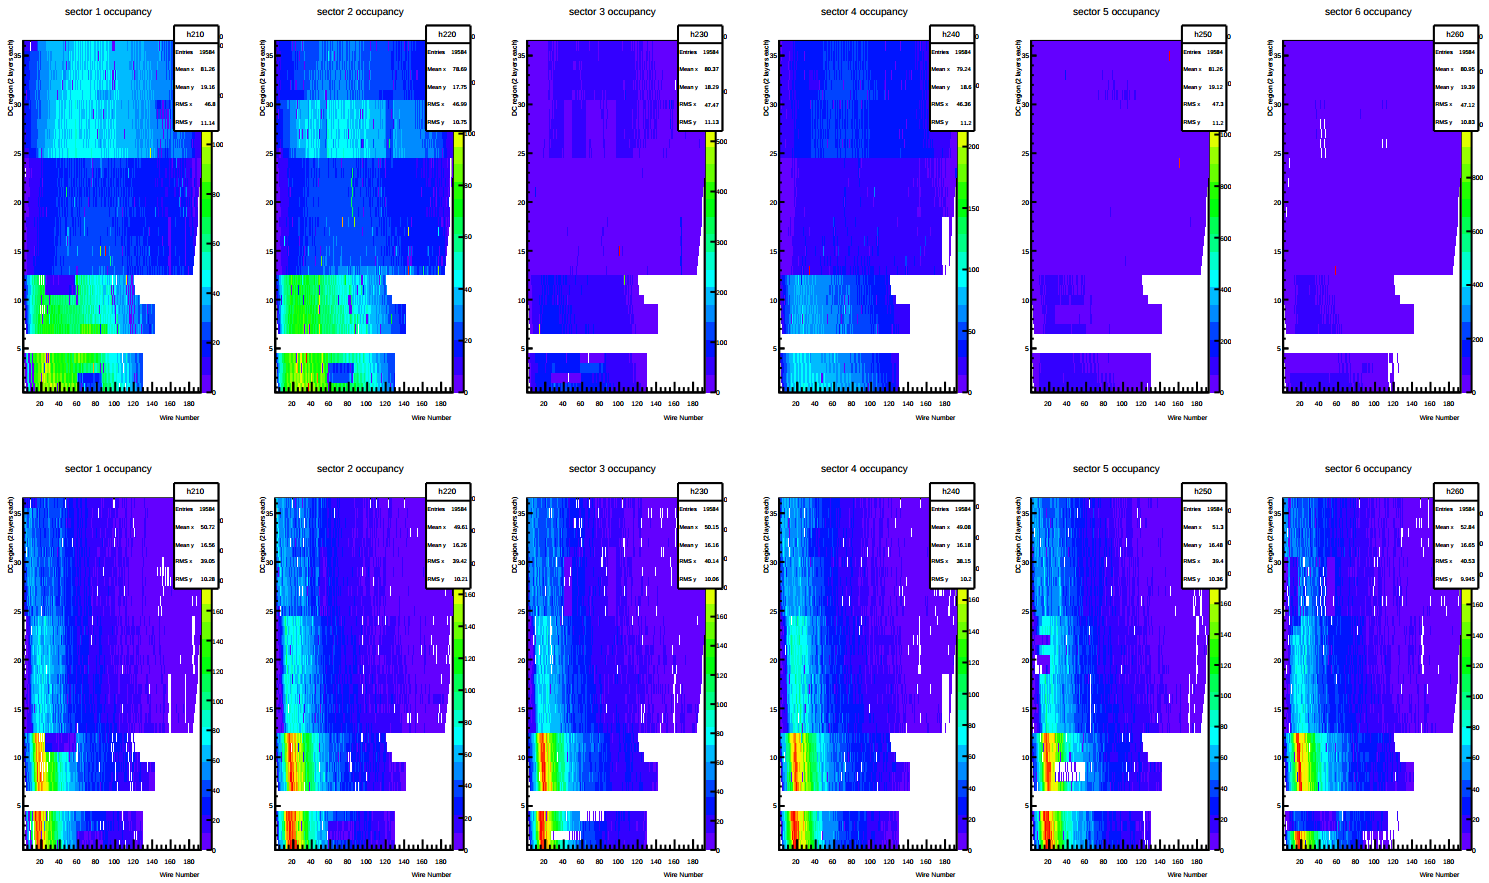
\includegraphics[width=8.5in]{figures/DCoccupancy.png}
\caption{A wire map of the DC occupancy for data (top row) and Monte Carlo (bottom row) for each sector (column 1 is sector 1, column 2 is sector 2, etc.). The holes are consistent between data and Monte Carlo confirming the efficacy of GPP.}
\label{fig:DCoccupancy}
\end{sidewaysfigure}
%

\subsection{Monte Carlo Reconstruction and Event Selection}
\label{subsec:ReconstructionAndEventSelection}
%
After the generated data has been passed through GSim and after the GSim output has been modified by GPP, this data is then cooked with RECSIS in the same was as the experimental data.
This produces an ntuple file where each event has a generated part and (possibly) a reconstructed part, the reconstructed part being identical in format to the cooked E1-F data files.
The reconstructed part is put through the same set of particle ID and fiducial cuts as the experimental data.
The cuts used here are not necessarily exactly identical to the experimental cuts, but they are the same kind of cuts; for example a $\mu \pm 3\sigma$ cut could produce slightly different cut values if $\mu$ and $\sigma$ are slightly different in the data and simulation.
Figure~\ref{fig:MC_pip_vvpCut} shows, as an example, the momentum dependent $\beta$ cut for $\pi^+$ ID for the reconstructed Monte Carlo; this should be compared to the experimental data version in figure~\ref{fig:pip_vvpCut}, which shows good agreement.
Also, figure~\ref{fig:phaseSpaceCoverage_recMC} shows the $x$-$Q^2$-$z$-$P_{h\perp}^2$ phase space of the reconstructed Monte Carlo; this should be compared to the experimental data version in figure~\ref{fig:binningScheme}, which shows good agreement.
Finally, both the generated and reconstructed Monte Carlo data is orgainzed into bins of $x$, $Q^2$, $z$, $P_{h\perp}^2$, and $\phi_h$ in the same way the data is.
%
\begin{figure}[htp]
\centering
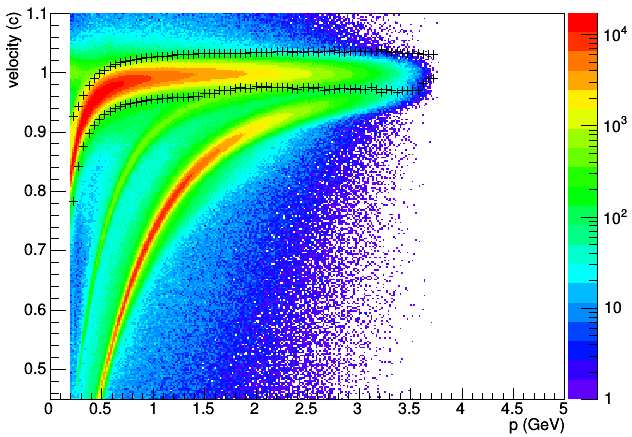
\includegraphics[width=4in]{figures/MC_pip_vvpCut.png}
\caption{The two dimensional view of the momentum dependent $\pi^+$ $\beta$ cut for the reconstructed Monte Carlo. This should be compared to the experimental data version in figure~\ref{fig:pip_vvpCut}.}
\label{fig:MC_pip_vvpCut}
\end{figure}
%
\begin{figure}[htp]
\centering
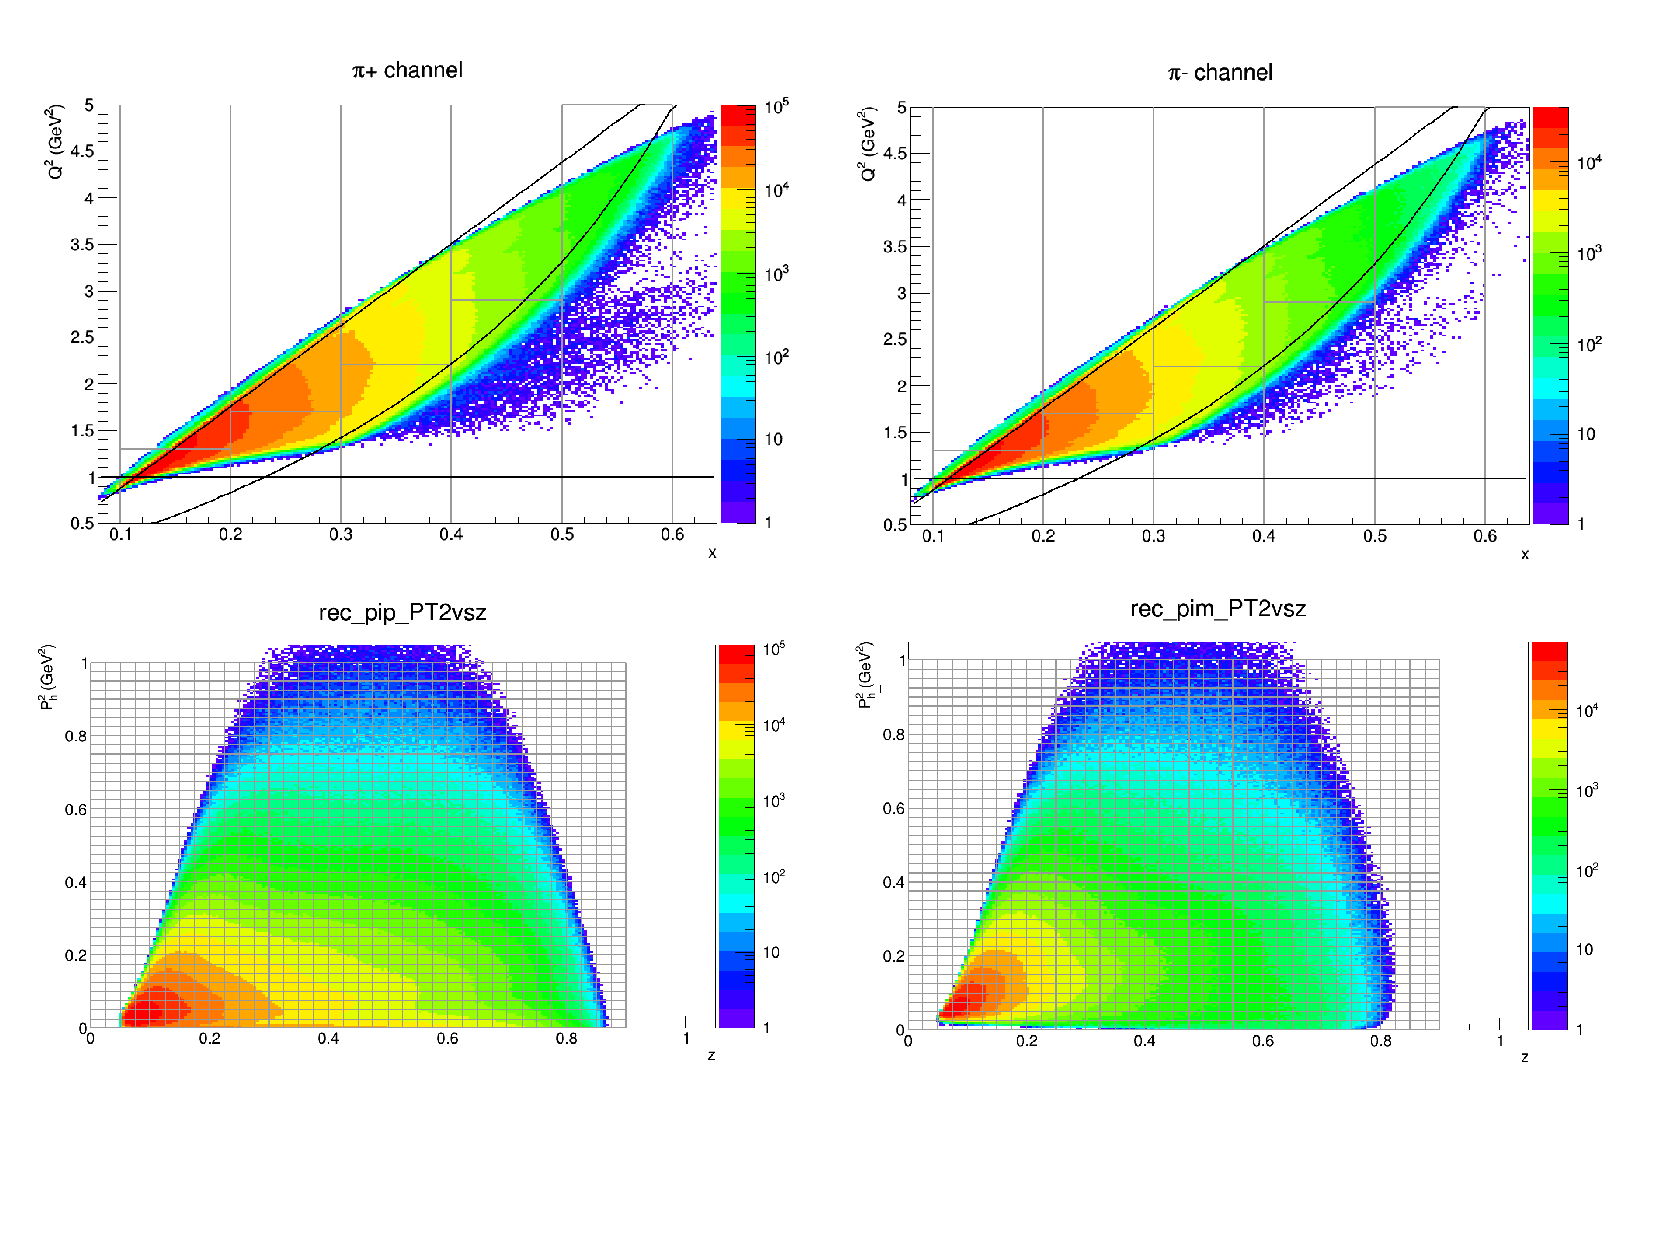
\includegraphics[width=5in]{figures/phaseSpaceCoverage_recMC.pdf}
\caption{$x$-$Q^2$ (top) and $z$-$P_{h\perp}^2$ (bottom) phase space coverage for the reconstructed Monte Carlo for the $\pi^+$ channel (left) ad the $\pi^-$ channel (right). This should be compared to the experimental data version in figure~\ref{fig:binningScheme}. Kinematic cuts are shown by black lines and the binning scheme is shown by gray lines.}
\label{fig:phaseSpaceCoverage_recMC}
\end{figure}
%

%
%%%%%%%%%%%%%%%%%%%%%%%%%%%%%%%%%%%%%%%%%%%%%%%%
%%%%%%%%%%%%%%%%%%%%%%%%%%%%%%%%%%%%%%%%%%%%%%%%

\clearpage % should prevent a backlog of figures from piling up

\section{Minimum $\phi_h$ Coverage for Reliable Fitting}
\label{sec:minPhihCoverage}
There are certain regions of phase space where the CLAS acceptance is zero.
The complex structure of this acceptance can be seen in figures~\ref{fig:zPT2_wPhih_n30to30deg_pip} ($\pi^+$) and~\ref{fig:zPT2_wPhih_n30to30deg_pim} ($\pi^-$), which show phase space coverge for events with $-30 < \phi_h < 30$ degrees.
These regions commonly occur around $\phi_h = 0$, potentially creating an occasion for unreliable results when fitting a particular $\phi_h$ distribution.
A study is therefore needed to check what is the minimum allowable coverage in $\phi_h$ for which $A_0$, $A_{UU}^{\cos\phi_h}$, and $A_{UU}^{\cos 2\phi_h}$ can be reliably extracted.
The criteria for $A_0$ will be different than the criteria for $A_{UU}^{\cos\phi_h}$ and $A_{UU}^{\cos 2\phi_h}$ since $A_0$ is a much more stable quantity.
%
\begin{sidewaysfigure}[htp]
\centering
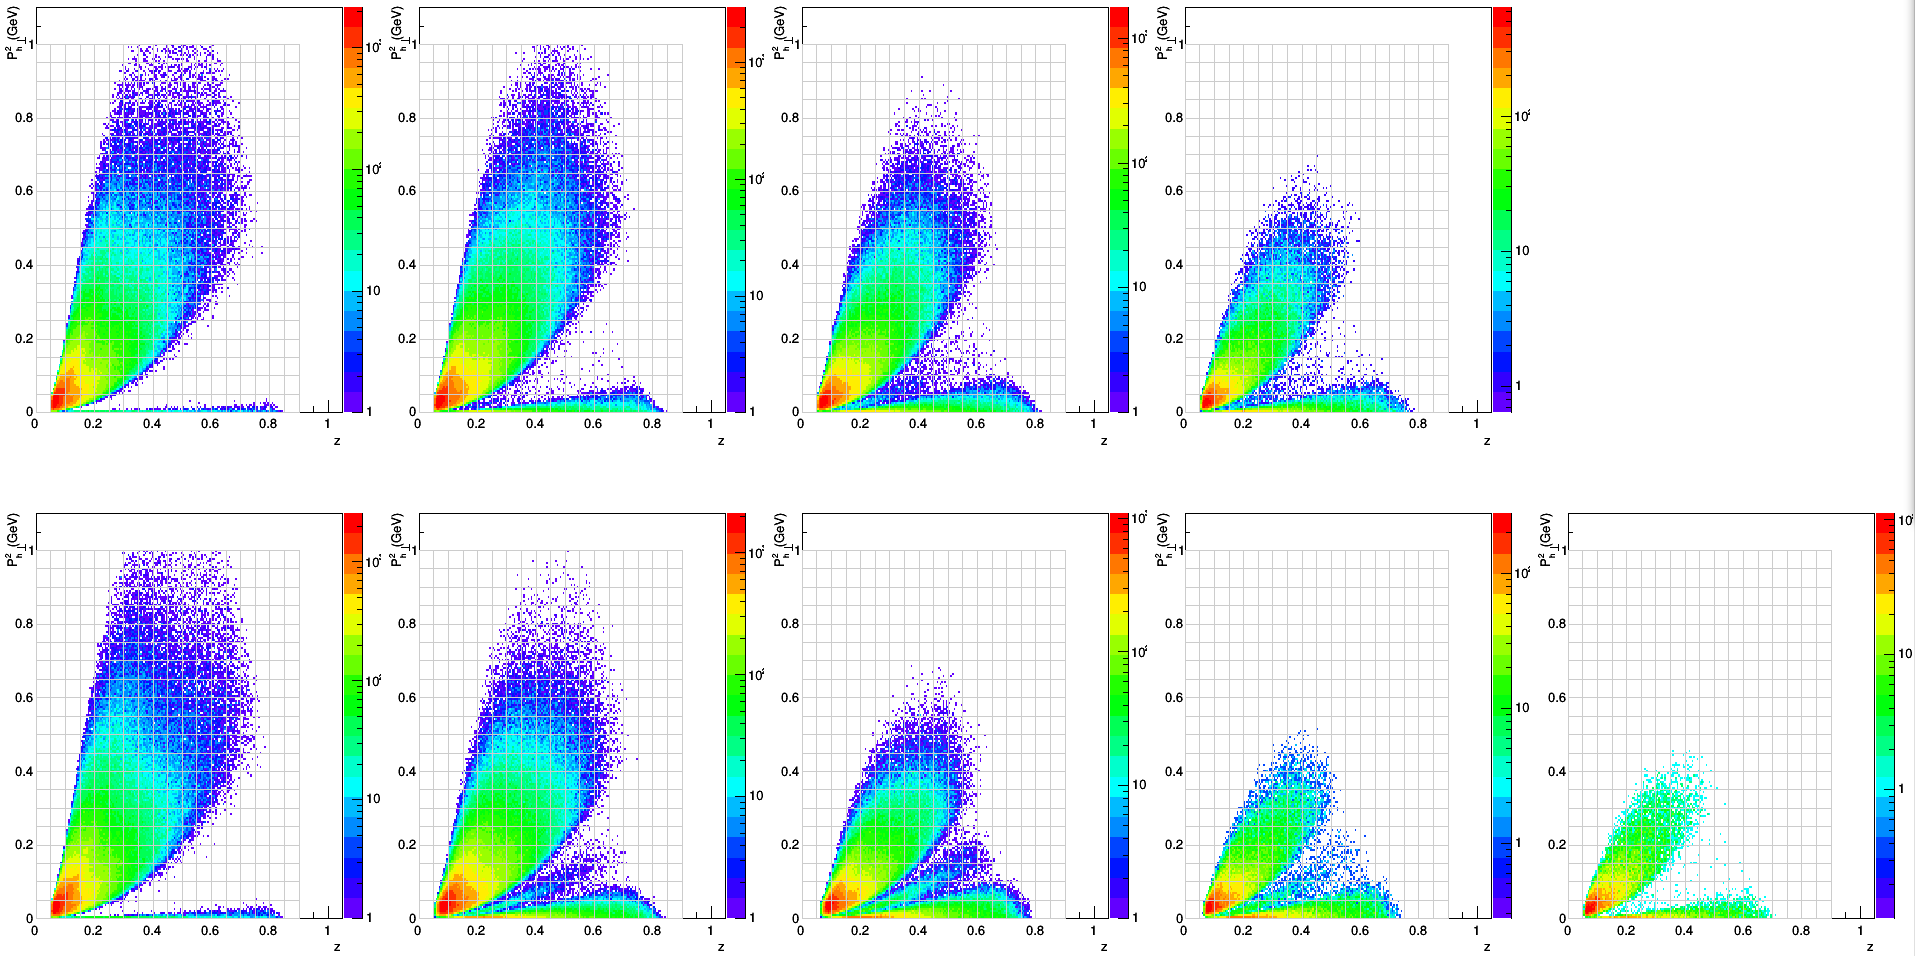
\includegraphics[width=8.5in]{figures/zPT2_wPhih_n30to30deg_pip.png}
\caption{$P_{h\perp}^2$ vs $z$ phase space coverage for the $\pi^+$ channel for events with $-30 < \phi_h < 30$ degrees. Columns are $x$ bins and rows are $Q^2$ bins.}
\label{fig:zPT2_wPhih_n30to30deg_pip}
\end{sidewaysfigure}
%
\begin{sidewaysfigure}[htp]
\centering
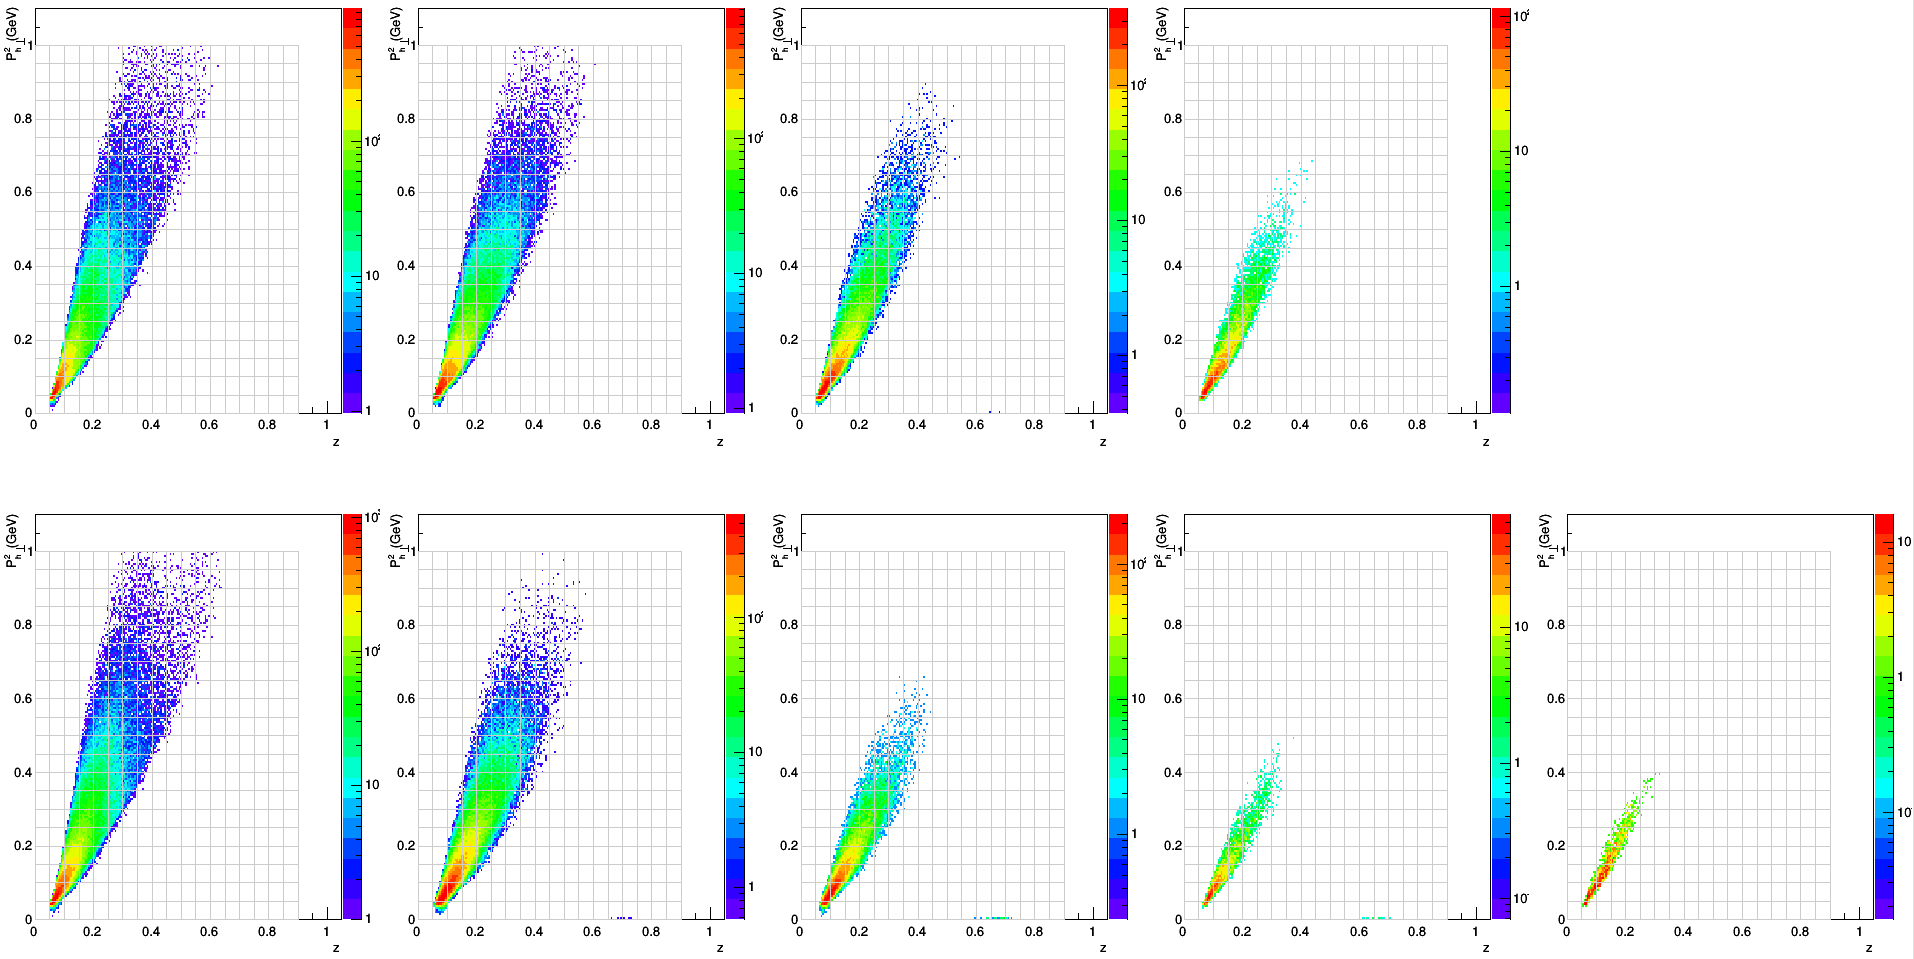
\includegraphics[width=8.5in]{figures/zPT2_wPhih_n30to30deg_pim.png}
\caption{$P_{h\perp}^2$ vs $z$ phase space coverage for the $\pi^-$ channel for events with $-30 < \phi_h < 30$ degrees. Columns are $x$ bins and rows are $Q^2$ bins.}
\label{fig:zPT2_wPhih_n30to30deg_pim}
\end{sidewaysfigure}
%

This study consisted of generating $\phi_h$ distributions with three options: the number of events to generate, the value of the $\cos\phi_h$ moment, and the value of the $\cos 2\phi_h$ moment.
The generated values of $A_{UU}^{\cos\phi_h}$ were -0.3, -0.2, -0.1, 0.0, 0.1, 0.2, and 0.3 (7 values).
Similarly, the generated values of $A_{UU}^{\cos 2\phi_h}$ were -0.3, -0.2, -0.1, 0.0, 0.1, 0.2, and 0.3 (7 values).
Finally, the number of generated events were 500, 1000, 2000, 5000, 10000, 20000, 50000, 100000, and 1000000 (9 values).
All $7 \times 7 \times 9 = 441$ combinations were produced.
Each distribution is then fit several times; each time a different range of $\phi_h$ around $0$ was first cut out.
An example of this can be seen in figure~\ref{fig:holeWidthStudyExample} which shows 5000 generated $\phi_h$ events with $A_{UU}^{\cos\phi_h} = -0.2$ and $A_{UU}^{\cos 2\phi_h} = 0.1$ and fit results; with each successive plot a larger range of $\phi_h$ around $0$ is cut out before fitting.
%
\begin{sidewaysfigure}[htp]
\centering
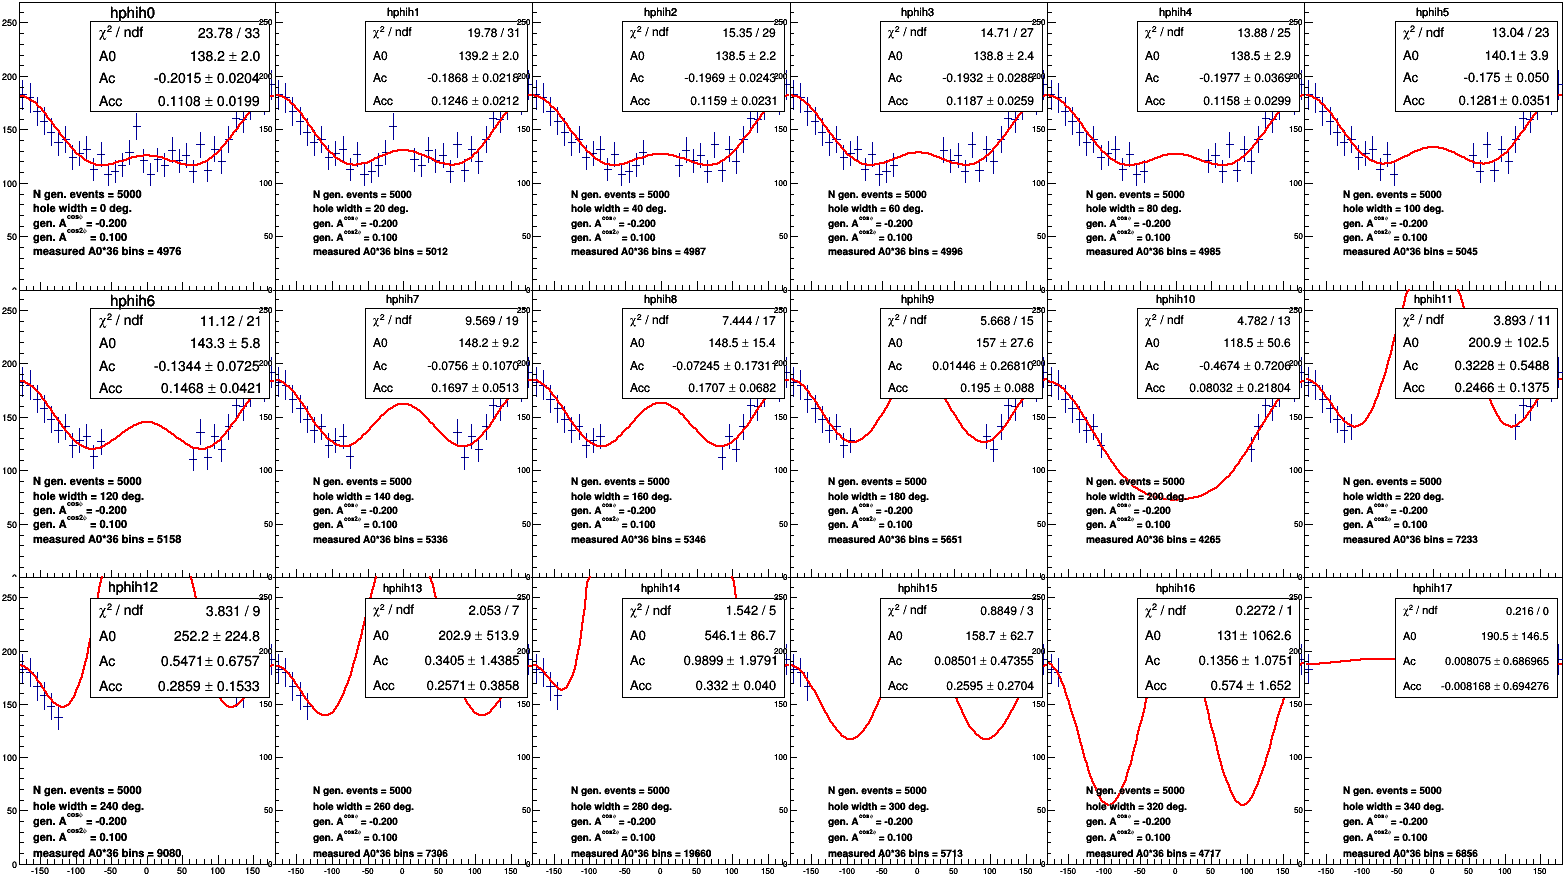
\includegraphics[width=8.5in]{figures/holeWidthStudyExample.png}
\caption{Generated $\phi_h$ distributions with fit results with different ranges of $\phi_h$ cut out around $0$. The top left plot has full $360^\circ$ coverage while the bottom right plot has only $10^\circ$ of coverage on each side. In this example 5000 events were generated with $A_{UU}^{\cos\phi_h} = -0.2$ and $A_{UU}^{\cos 2\phi_h} = 0.1$.}
\label{fig:holeWidthStudyExample}
\end{sidewaysfigure}

As expected, higher statistics distributions produce more stable fit results.
Within common sense limitations, a worst-case-scenario should be used as the criteria; anything less conservative could produce unreliable results.
Furthermore, generated distributions are always much more ideal than experimental results.
The case of 2000 generated events with $A_{UU}^{\cos\phi_h} = -0.2$ and $A_{UU}^{\cos 2\phi_h} = 0.0$ is used as a representative example.
The results for this case are summarized in figure~\ref{fig:holeWidthStudySummary}.
It is clear that the fit results become very volatile with a hole width greater than $60^\circ$ (i.e. events between $-30^\circ$ and $30^\circ$ are cut).
%
\begin{figure}[htp]
\centering
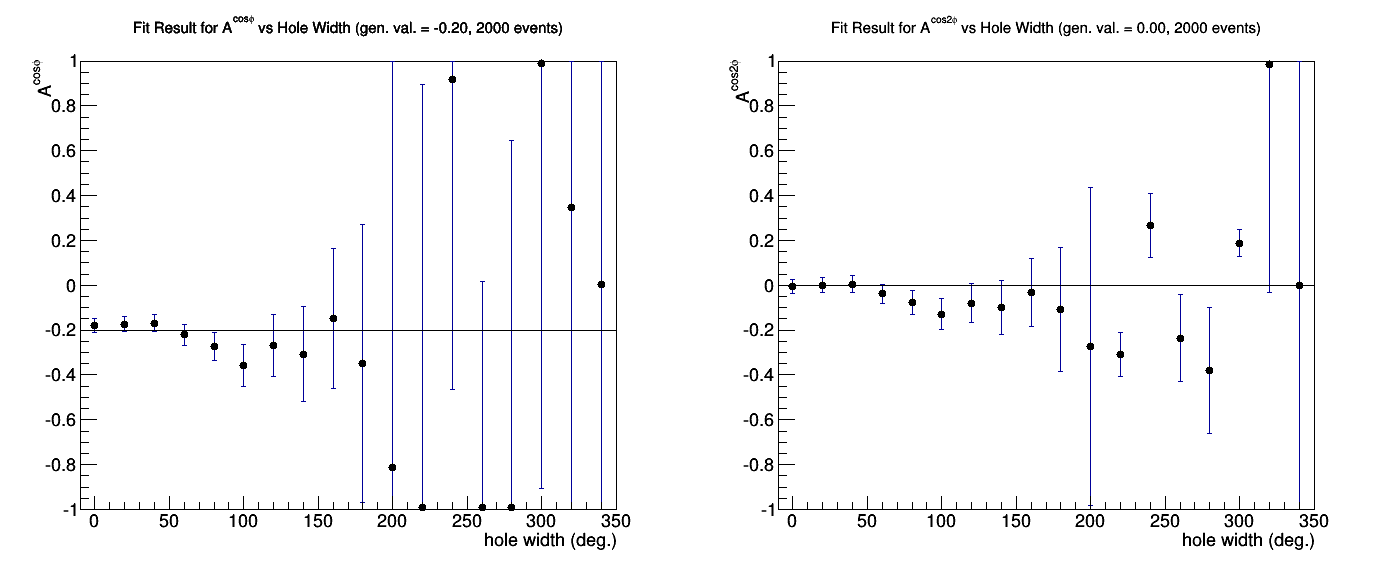
\includegraphics[width=6in]{figures/holeWidthStudySummary.png}
\caption{$A_{UU}^{\cos\phi_h}$ (left) and $A_{UU}^{\cos 2\phi_h}$ (right) extracted from the fit of the generated $\phi_h$ distribution as a function of the width of the zero acceptance hole. The black horizontal lines show the generated values.}
\label{fig:holeWidthStudySummary}
\end{figure}

As a result of this study, $A_{UU}^{\cos\phi_h}$ and $A_{UU}^{\cos 2\phi_h}$ are not measured in bins where there is an acceptance hole in $\phi_h$ greater than $60^\circ$ in width.
For measuring $A_0$, at least $100^\circ$ of coverage is required.


\chapter{Radiative Corrections}
\label{cha:RadiativeCorrections}
%
When a cross-section is measured experimentally, the measurement yields the radiated cross-section plus contributions from radiated exclusive events, not the desired Born cross-section.
There are seven leading order contributions to the measured cross-section, summarized in figure~\ref{fig:radiatedFeynmanDiagrams}.
It is difficult, if not impossible, to distinguish these processes on the level of event selection, radiative corrections are therefore needed.
HAPRAD version 2.0 \cite{Akushevich99}\cite{Akushevich09} was used to calculate radiative corrections.
%
\begin{figure}[htp]
\centering
\includegraphics[width=5in]{figures/radiatedFeynmanDiagrams_BandW.png}
\caption{Feynman diagrams for contributions to the radiative cross-section. (a) The Born cross-section, (b) and (c) the emission of a radiated photon for SIDIS processes, (d) and (e) loop diagrams, and (f) and (g) emission of a radiated photon for exclusive processes.}
\label{fig:radiatedFeynmanDiagrams}
\end{figure}

HAPRAD works by calculating $\sigma_{rad+tail} \left( x, Q^2, z, P_{h\perp}^2, \phi_h \right)$ for a given \allowbreak $\sigma_{Born} \left( x, Q^2, z, P_{h\perp}^2, \phi_h \right)$ which is obtained from a model.
The radiative correction factor is then simply
\begin{equation}
\label{eq:RCfactor}
RC\ factor \left( x, Q^2, z, P_{h\perp}^2, \phi_h \right) = \frac{\sigma_{rad+tail} \left( x, Q^2, z, P_{h\perp}^2, \phi_h \right)}{\sigma_{Born} \left( x, Q^2, z, P_{h\perp}^2, \phi_h \right)}
\end{equation}
and the Born cross-section can be obtained by dividing the measured cross-section by the RC factor, i.e., $\sigma_{Born} = \sigma_{measured}/\text{RC factor}$.
Three different models were used to study model dependence, which proved to be a small effect (see chapter~\ref{cha:SystematicUncertainties} which discusses systematic uncertainties).
The three models used were (1) $A_{UU}^{\cos \phi_h} = A_{UU}^{\cos 2\phi_h} = 0$, (2) the ``default'' model that came with HAPRAD, which proved to describe the data reasonably well, and (3) an improved model based on the default model but with the parameters tuned to better match the data.
Model 3 was used for the final results and is shown for several bins in figures~\ref{fig:hapradModel_data_compare_pip} ($\pi^+$ channel) and~\ref{fig:hapradModel_data_compare_pim} ($\pi^-$ channel) along with the final results for comparison.
In the figures, the top row shows $A_{UU}^{\cos \phi_h}$ vs $P_{h\perp}^2$ and the bottom row shows $A_{UU}^{\cos 2\phi_h}$ vs $P_{h\perp}^2$; the columns are bins of $z$.
%
\begin{sidewaysfigure}[htp]
\centering
\includegraphics[width=8.5in]{figures/hapradModel_data_compare_pip.pdf}
\caption{The model for the Born cross-section used in HAPRAD (black points) and the experimental results (red points) for the $\pi^+$ channel. The top row shows $A_{UU}^{\cos \phi_h}$ vs $P_{h\perp}^2$ and the bottom row shows $A_{UU}^{\cos 2\phi_h}$ vs $P_{h\perp}^2$; the columns are bins of $z$. These results are for the high $Q^2$ of $ 0.1 < x < 0.2$.}
\label{fig:hapradModel_data_compare_pip}
\end{sidewaysfigure}
%
\begin{sidewaysfigure}[htp]
\centering
\includegraphics[width=8.5in]{figures/hapradModel_data_compare_pim.pdf}
\caption{The model for the Born cross-section used in HAPRAD (black points) and the experimental results (red points) for the $\pi^-$ channel. The top row shows $A_{UU}^{\cos \phi_h}$ vs $P_{h\perp}^2$ and the bottom row shows $A_{UU}^{\cos 2\phi_h}$ vs $P_{h\perp}^2$; the columns are bins of $z$. These results are for the high $Q^2$ of $ 0.1 < x < 0.2$.}
\label{fig:hapradModel_data_compare_pim}
\end{sidewaysfigure}
%

Some results from HAPRAD are shown in figures~\ref{fig:RCmagnitude_4D_intPhih} and~\ref{fig:RC_zPT2grid_x0QQ0}.
Figure~\ref{fig:RCmagnitude_4D_intPhih} shows the magnitude of the RC factor (integrated over $\phi_h$) as a function of $z$ and $P_{h\perp}^2$ for each of the nine $x$-$Q^2$ bins.
These results are very reasonable as they don't deviate very far from unity within the relevant kinematic ranges.
The kinematic region highlighted by the red rectangle in the bottom-left plot of figure~\ref{fig:RCmagnitude_4D_intPhih} is shown in more detail in figure~\ref{fig:RC_zPT2grid_x0QQ0}, which shows the $\phi_h$ dependence of $\sigma_{Born}$ (obtained from a model), $\sigma_{rad}$, and $\sigma_{tail}$ at different values of $z$ and $P_{h\perp}^2$ for fixed $x$ and $Q^2$.
%
\begin{sidewaysfigure}[htp]
\centering
\includegraphics[width=8.5in]{figures/RCmagnitude_4D_intPhih.png}
\caption{$\int \sigma_{rad+tail} d\phi_h / \int \sigma_{Born} d\phi_h$ as a function of $z$ and $P_{h\perp}^2$ for each of the nine $x$-$Q^2$ bins.}
\label{fig:RCmagnitude_4D_intPhih}
\end{sidewaysfigure}
%
\begin{sidewaysfigure}[htp]
\centering
\includegraphics[width=8.5in]{figures/RC_zPT2grid_x0QQ0.png}
\caption{$\sigma_{Born}$ (blue), $\sigma_{rad}$ (red), and $\sigma_{tail}$ (teal) vs $phi_h$ for several points in $z$ and $P_{h\perp}^2$ and fixed $x$ and $Q^2$.}
\label{fig:RC_zPT2grid_x0QQ0}
\end{sidewaysfigure}

\chapter{Bin Centering Corrections}
\label{cha:BCC}
%
When the cross-section is measured in 5-dimensional bins of $x$, $Q^2$, $z$, $P_{h\perp}^2$, and $\phi_h$, the result is the cross-section averaged over the phase space coverage of each bin (see figure~\ref{fig:BCC_basicExample}).
A more desirable quantity is the cross-section at the center point of the bin; therefore, bin centering corrections are applied.
%
\begin{figure}[htp]
\centering
\includegraphics[width=3in]{figures/BCC_basicExample.png}
\caption{An example illustrating that the center point of a function (red point) can differ from the average value (green point).}
\label{fig:BCC_basicExample}
\end{figure}

Bin centering corrections are approximated using a model based on the results of the measurement.
Using the model, the cross-section is calculated in ``micro-bins'' (bins much smaller than the bins used for the final analysis, referred to here as ``normal bins''), the bin centering correction factor for a particular normal bin is then given by
\begin{equation}
\label{eq:BCCequation}
BCC\ factor = \frac{v}{V} \frac{\sigma_{averaged}}{\sigma_{center}}
\end{equation}
where $v$ is the 5-dimensional ``volume'' of the micro-bin at the center of the normal bin, $V$ is the volume the normal bin, $\sigma_{averaged}$ is the cross-section averaged over the normal bin, and $\sigma_{center}$ is the cross-section at the micro-bin at the center of the normal bin.

The micro-binning scheme is as follows: 90 $z$ bins from 0.0-0.9, 100 $P_{h\perp}^2$ bins 0.0-1.0 $GeV^2$, 50 $x$ bins from 0.1-0.6, 50 $Q^2$ bins from 1.0-5.0 $GeV^2$, 180 $\phi_h$ bins from -180-180 degrees.

\clearpage

\chapter{Systematic Uncertainties}
\label{cha:SystematicUncertainties}

Since it is not always possible to determine the ideal set of values for a particular analytical technique, estimates of systematic errors are performed here.
This is done by making small variations to a particular value, while holding the rest constant, and looking at how the end results change.
14 sources of systematic errors are studied (labeled 0-13), the first 13 are given in table~\ref{tab:sysErrorSources} along with the number of variations and description for each source.
The 14th source of systematic error is variations in the 6 sectors of CLAS; a separate section below is dedicated to this topic.

\section{Sector Dependence}
\label{sec:SectorDependence}
In reality, the 6 sectors of CLAS are not identical.
To account for this, sector dependence is included in the systematic error studies.
As can be seen in figure~\ref{fig:sectorDep_0_1_4_3}, the variations are both statistical and systematic.
To avoid double counting the statistical error, the total error is assumed to be:
%
\begin{equation}
\label{eq:totalError_stat_sys}
\sigma^2 = \sigma^2_{stat} + \sigma^2_{sys}
\end{equation}
%
and the systematic error is then simply:
%
\begin{equation}
\label{eq:sysError_sectorDep}
\sigma^2_{sys} = \sigma^2 - \sigma^2_{stat}.
\end{equation}
%
In some cases $\sigma^2_{stat}$ is larger than $\sigma^2$.
Figure~\ref{fig:normalAndException_sectorSystematics} shows a ``normal'' example (left) and and example when $\sigma^2_{stat} > \sigma^2$ (right).
When this happens the systematic error is taken to be the average of all the bins.
Figure~\ref{fig:distributionOfSectorSystematics} shows the distributions of sector systematic errors for $A_0$, $A^{\cos\phi}$, and $A^{\cos 2\phi}$ for $\pi^+$ and $\pi^-$ along with the averages used for $\sigma^2_{sys} = 0$ when $\sigma^2_{stat} > \sigma^2$.
%
\begin{figure}[htp]
\centering
\includegraphics[width=6in]{figures/sectorDep_1_1_6_8.png}
\caption{Measurements of $A_0$ (left), $A^{\cos\phi}$ (middle), and $A^{\cos2\phi}$ (right) for a representitive bin as a function of the electron sector for $\pi+$ (red circles) and $\pi-$ (blue triangles). This kinematic bin is the high $Q^2$ bin of $0.2 < x < 0.3$, $0.3 < z < 0.35$, and $0.4 < P_{h\perp}^2 < 0.45$ $GeV^2$.}
\label{fig:sectorDep_0_1_4_3}
\end{figure}
%
\begin{figure}[htp]
\centering
\includegraphics[width=6in]{figures/normalAndException_sectorSystematics.png}
\caption{Example of a ``normal'' case (left) where the fluctuation of the points is due to both statistical and systematic uncertainty, and a case where the fluctuation of the points is fully accounted for by statistical uncertainty alone (i.e. $\sigma^2_{stat} > \sigma^2$) (right).}
\label{fig:normalAndException_sectorSystematics}
\end{figure}
%
\begin{figure}[htp]
\centering
\includegraphics[width=6in]{figures/distributionOfSectorSystematics.png}
\caption{The distributions of sector systematic errors for $A_0$ (left), $A^{\cos\phi}$ (middle), and $A^{\cos 2\phi}$ (right) for $\pi^+$ (top) and $\pi^-$ (bottom).}
\label{fig:distributionOfSectorSystematics}
\end{figure}

\section{Other Sources of Systematic Uncertainty}
\label{sec:OtherSystematicUncertainty}
The systematic error on the final result due to a given source is the RMS of the deviations of the modified result from the original, i.e. the error from source $i$ is
%
\begin{equation}
\label{eq:RMS}
\Delta_{RMS}^i = \frac{\sqrt{\sum_j^{N_v^i} \Delta_j^2}}{\sqrt{N_v^i}}
\end{equation}
%
where $\Delta_j$ is the difference between the final result with the nominal value and the final result with variation $j$, and $N_v^i$ is the number of variations for source $i$.
``Final result'' refers to the values of $A_0$, $A_{UU}^{\cos\phi_h}$, and $A_{UU}^{\cos 2\phi_h}$ for each kinematic bin (systematic errors are calculated for each quantity).
The sources of systematic error are assumed to be uncorrelated and therefore are added in quadrature to get the total systematic error.
In the case of a cut value, there are two variations: a looser cut and a tighter cut.
In the case of model dependence, there is one variation: the second to last iteration.
%
\begin{table}[htp]
\centering
%\begin{tabular}{c l c l}
\begin{tabular}{ p{1.5cm} p{3cm} p{2cm} p{6cm} }
\hline
\textbf{Label} & \textbf{Source} & \textbf{\# of variations} & \textbf{Description}\\ \hline
0 & e- z-vertex cut & 2 & cut value is loosened or tightened by 0.2 cm on each side \\
1 & e- EC sampling cut & 2 & see figure~\ref{fig:eSystematicCuts} \\
2 & e- EC outer vs inner cut & 2 & cut value is loosened or tightened by 0.005 GeV \\
3 & e- EC geometric cut & 2 & see figure~\ref{fig:eSystematicCuts} \\
4 & e- CC $\theta$ matching cut & 2 & see figure~\ref{fig:eSystematicCuts} \\
5 & e- region 1 fiducial cut & 2 & see figure~\ref{fig:eSystematicCuts} \\
6 & e- region 3 fiducial cut & 2 & see figure~\ref{fig:eSystematicCuts} \\
7 & e- CC fiducial cut & 2 & see figure~\ref{fig:eSystematicCuts} \\
8 & pion $\beta$ cut & 2 & cut is loosened or tightened by $0.25\sigma$ on both the low and high side \\
9 & pion region 1 fiducial cut & 2 & see figure~\ref{fig:pionSystematicCuts} \\
10 & $\phi_h$ fiducial cut & 2 & a bin ($10^\circ$) on each side is added or removed \\
11 & acceptance model dependence & 1 & the second to last iteration is used \\
12 & radiative correction model dependence & 1 & the second to last iteration is used \\
\hline
\end{tabular}
\caption{13 of the 14 sources of systematic error studied. The other source is sector dependence, which is handled separately.}
\label{tab:sysErrorSources}
\end{table}
%
\begin{sidewaysfigure}[htp]
\centering
\includegraphics[width=8.5in]{figures/eSystematicCuts.png}
\caption{The loose, nominal, and tight cuts for six electron ID plots used for calculating systematic errors.}
\label{fig:eSystematicCuts}
\end{sidewaysfigure}
%
\begin{figure}[htp]
\centering
\includegraphics[width=6in]{figures/pionSystematicCuts.png}
\caption{The loose, nominal, and tight cuts for the region 1 fiducial cut for $\pi^+$ (left) and $\pi^-$ (right) used for calculating systematic errors.}
\label{fig:pionSystematicCuts}
\end{figure}
%
Figure~\ref{fig:systematicErrors_representitiveBin} shows the systematic error contribution of each source on $A_0$, $A_{UU}^{\cos\phi_h}$, and $A_{UU}^{\cos 2\phi_h}$ for a representitive bin.
%
\begin{figure}[htp]
\centering
\includegraphics[width=6in]{figures/allSystematics_1_1_7_7.png}
\caption{Systematic errors on $A_0$ (left), $A_{UU}^{\cos\phi_h}$ (middle), and $A_{UU}^{\cos 2\phi_h}$ (right) for each source for a representitive bin for the $\pi+$ channel. The first 13 sources are summarized in table~\ref{tab:sysErrorSources}, the 14th source is sector dependence. This kinematic bin is the high $Q^2$ bin of $0.2 < x < 0.3$, $0.35 < z < 0.4$, and $0.35 < P_{h\perp}^2 < 0.4$ $GeV^2$.}
\label{fig:systematicErrors_representitiveBin}
\end{figure}
%

\clearpage

\chapter{$A_0$, $A_{UU}^{\cos\phi_h}$, and $A_{UU}^{\cos 2\phi_h}$}
\label{cha:A0AcAcc}

After events have been selected and binned, and after all corrections have been applied, the $\phi_h$ distributions for each $x-Q^2-z-P_{h\perp}^2$ bin are fit with the function $a(1 + b\cos\phi_h + c\cos 2\phi_h)$.
The parameters $a$, $b$, and $c$ then directly give $A_0$, $A_{UU}^{\cos\phi_h}$, and $A_{UU}^{\cos 2\phi_h}$ for each $x-Q^2-z-P_{h\perp}^2$ bin.
A complete table of results can be found in the ancillary files.
Several representitive plots are shown here in figure~\ref{fig:A0AcAcc_zPT2bins_x1QQ1_final}, which shows $A_0$, $A_{UU}^{\cos\phi_h}$, and $A_{UU}^{\cos 2\phi_h}$ vs $P_{h\perp}^2$ for several $z$ bins for both pion channels.
Several of the fits used to obtain figure~\ref{fig:A0AcAcc_zPT2bins_x1QQ1_final} are shown in figure~\ref{fig:phihFits_PT2bins_x1QQ1z6_final}.
%
\begin{figure}[htp]
\centering
\vspace{-1.5cm}
\makebox[\textwidth][c]{\includegraphics[width=6.5in]{figures/A0AcAccVPT2_x1QQ1z6.png}} % this centers it more nicely
\makebox[\textwidth][c]{\includegraphics[width=6.5in]{figures/A0AcAccVPT2_x1QQ1z7.png}} % this centers it more nicely
\makebox[\textwidth][c]{\includegraphics[width=6.5in]{figures/A0AcAccVPT2_x1QQ1z8.png}} % this centers it more nicely
\makebox[\textwidth][c]{\includegraphics[width=6.5in]{figures/A0AcAccVPT2_x1QQ1z9.png}} % this centers it more nicely
\caption{$A_0$ (left column), $A_{UU}^{\cos\phi_h}$ (middle column), and $A_{UU}^{\cos 2\phi_h}$ (right column) vs $P_{h\perp}^2$ for $\pi+$ (red circles) and $\pi-$ (blue triangles). The $x$-$Q^2$ bin is fixed (the high $Q^2$ of $0.2 < x < 0.3$). Several $z$ bins are shown: $0.30 < z < 0.35$ (top row), $0.35 < z < 0.40$ (second row), $0.40 < z < 0.45$ (third row), $0.45 < z < 0.50$ (bottom row).}
\label{fig:A0AcAcc_zPT2bins_x1QQ1_final}
\end{figure}
%
\begin{figure}[htp]
\centering
\vspace{-1.5cm}
\makebox[\textwidth][c]{\includegraphics[width=6.5in]{figures/phihFits_PT2bins_x1QQ1z6_final.pdf}} % this centers it more nicely
\caption{Fits of several of the $\phi_h$ distrubutions used to obtain figure~\ref{fig:A0AcAcc_zPT2bins_x1QQ1_final}. The rows are bins of $P_{h\perp}^2$ as shown by the large axis on left. $\pi^+$ results are shown in the left column and $\pi^-$ on the right. These results are from the high $Q^2$ bin of $0.2 < x < 0.3$ and $0.3 < z < 0.35$.}
\label{fig:phihFits_PT2bins_x1QQ1z6_final}
\end{figure}
%
\clearpage

\chapter{Comparison to Other Data}
\label{cha:Comparison}

A similar measurement has been published by the CLAS Collaboration using \mbox{E1-6} data~\cite{Osipenko09}.
However, it only measures the $\pi^+$ channel and has a more limited kinematic range.
A comparison for the $\pi^+$ channel in overlapping kinematic ranges is done here.
In order to have a meaningful comparison, the binning scheme used here was temporarily changed to match that of~\cite{Osipenko09}.
Figure~\ref{fig:osipenkoComparisonVPT2_2zBins} shows the comparison between E1-f (red points) and E1-6 (black points) as a function of $P_{h\perp}^2$ for two $z$ bins ($0.29 < z < 0.32$ (left column) and $0.32 < z < 0.35$ (right column)) for the $\pi^+$ channel.
The results show clear agreement, both qualitatively and quantitatively, implying good consistency between measurements.
%
\begin{sidewaysfigure}[htp]
\centering
\includegraphics[width=8.5in]{figures/osipenkoComparisonVPT2_2zBins.png}
\caption{$A_{UU}^{\cos \phi_h}$ (top row) and $A_{UU}^{\cos 2\phi_h}$ (bottom row) vs $P_{h\perp}^2$ for two $z$ bins ($0.29 < z < 0.32$ (left column) and $0.32 < z < 0.35$ (right column)) for the $\pi^+$ channel for E1-f (red points) and E1-6 (black points). Only the statistical error bars are shown here.}
\label{fig:osipenkoComparisonVPT2_2zBins}
\end{sidewaysfigure}
%
\clearpage

 % experimental (HERMES, Osipenko) and theoretical?
\chapter{Conclusion}
\label{cha:Conclusion}

The $\cos\phi_h$ moment, $\cos 2\phi_h$ moment, and $\phi$-independent term of the unpolarized SIDIS cross-section have been measured for both charged pion channels in a fully differential way with good statistics over a wide kinematic range ($0.1 < x < 0.6$, $1.0 < Q^2 < 4.7\ \text{GeV}^2$, $0.0 < z < 0.9$, $0.0 < P_{h\perp}^2 < 1.0\ \text{GeV}^2$, $-180^\circ < \phi_h < 180^\circ$).
The $\cos\phi_h$ and $\cos 2\phi_h$ modulations show a clear dependence on flavor which hints at a non-zero Boer-Mulders effect~\cite{Gamberg08}\cite{Barone08}\cite{Zhang08}\cite{Barone10} and could give insights into the quark orbital angular momentum ($L_q$) contribution of the proton spin; but more intensive theoretical comparisons, which are currently in progress, are needed first.
Results show a reasonable agreement with a previous CLAS measurement in overlapping kinematics.

The study of nucleon structure via the accessing of TMDs is a major thrust of up-and-coming nuclear physics projects such as CLAS12~\cite{Burkert08} and the proposed Electron-Ion Collider (EIC)~\cite{Boer11}.
A CLAS Collaboration proposal to continue studies of the Boer-Mulders function at higher energies at CLAS12 has been given the highest priority rating by PAC 30~\cite{Avakian06}.
Many of the challenges associated with precision measurements of this type have been addressed here.
Furthermore, the two experiments (this one and the future one at CLAS12) will have some overlapping kinematics and some unique kinematics, and therefore this analysis will be valuable both in its own right and for comparison purposes.
In conclusion, the work described in this dissertation has improved our understanding of this field and provided a solid foundation for future advancements.



% All the references are located in here
\begin{thebibliography}{99}

\bibitem{hofstader56}
	R.W. McAllister and R. Hofstader,
	Phys. Rev. \textbf{102}, 851 (1956).

\bibitem{hofstader58}
	M.R. Yearian and R. Hofstader,
	Phys. Rev. \textbf{110}, 552 (1958).

\bibitem{gellmann61}
	M. Gell-Mann, ``The Eightfold Way: A Theory of Strong Interaction Symmetry,''
	Caltech Synchrotron Laboratory Report No. CTSL-20 (1961).

\bibitem{neeman61}
	Y. Ne'eman, 
	Nucl. Phys. \textbf{26}, 222 (1961).

\bibitem{gellmann64}
	M. Gell-Mann,
	Phys. Lett. \textbf{8}, 214 (1964).

\bibitem{zweig64}
	G. Zweig, ``An SU$_{3}$ Model for Strong Interaction Symmetry and Its Breaking,''
	CERN Report No. TH 412 (Geneva, 1964).

\bibitem{zweig65}
	G. Zweig, ``Fractionally Charged Particles and $SU_{6}$,''
	Symmetries in Elementary Particle Physics (Academic Press, New York, 1965), p. 192.

\bibitem{SLAC66}
	SLAC-MIT-CIT Collaboration, ``Proposals for Initial Electron Scattering Experiments Using the SLAC Spectrometer Facilities,''
	Stanford Linear Accelerator Center Proposal No.4 (January 1966)

\bibitem{bjorken69}
	J.D. Bjorken and E.A. Paschos, ``Inelastic Electron Proton and gamma Proton Scattering, and the Structure of the Nucleon,''
	Phys. Rev. \textbf{185}, 1975 (1969).

\bibitem{feynman69}
	R.P. Feynman, ``Very High-Energy Collision of Hadrons,''
	Phys. Rev. Lett. \textbf{23}, 1415 (1969).

\bibitem{NNPDF13}
	C. S. Deans, ``Progress in the NNPDF Global Analysis,''
	hep-ph/1304.2781 (2013).

\bibitem{EMC88}
	European Muon Collaboration, ``A measurement of the spin asymmetry and determination of the structure function $g_1$ in deep inelastic muon-proton scattering,''
	Phys. Rev. B, Vol. 206, Issue 2, 364-370 (1988).

\bibitem{Collins02}
	J. C. Collins, ``Leading twist single transverse-spin asymmetries: Drell-Yan and deep inelastic scattering,''
	Phys. Lett. B536 43-48, (2002).

\bibitem{Pasquini10}
	B. Pasquini, ``Sivers and Boer-Mulders functions in Light-Cone Quark Models,''
	Phys. Rev. D81 114013, (2010).

\bibitem{Jaffe96}
	R.L. Jaffe, ``Spin, Twist and Hadron Structure in Deep Inelastic Processes,''
	hep-ph/9602236 (1996).

\bibitem{Boer98}
	D. Boer and P.J. Mulders, Phys. Rev. \textbf{D57},
	5780 (1998), hep-ph/9711485.

\bibitem{Bacchetta04}
	A. Bacchetta, U. D'Alesio, M. Diehl, and C. A. Miller, Phys. Rev. \textbf{D70},
	117504 (2004), hep-ph/0410050.

\bibitem{Bacchetta07}
	A. Bacchetta \emph{et al.}, JHEP 0702:093 (2007), hep-ph/0611265v2.

\bibitem{Collins88}
	J. C. Collins, D. E. Soper, and G. Sterman, ``Factorization of Hard Processes in QCD,''
	Adv. Ser. Direct. High Energy Phys., 5:1-91, (1988).

\bibitem{Sterman95}
	G. Sterman \emph{et al.}, ``Handbook of perturbative QCD,''
	Rev. Mod. Phys., 67(1):157-248, (1995).

\bibitem{Mecking03}
	B. Mecking \emph{et al.}, Nucl. Inst. Meth. \textbf{A505}, 2003.

\bibitem{Airapetian05}
	A. Airapetian \emph{et al.}, Phys. Rev. Lett. 94 012002 (2005).

\bibitem{Miller07}
	G. A. Miller, Phys. Rev. C 76 065209 (2007).

\bibitem{Jacob97}
	R. Jacob, P. J. Mulders, and J. Rodrigues, Nucl. Phys. \textbf{A626}, 937 (1997).

\bibitem{Pasquini08}
	B. Pasquini, S. Cazzaniga, and S. Boffi, Phys. Rev. \textbf{D78}, 034025 (2008).

\bibitem{Bacchetta08}
	A. Bacchetta, F. Conti, and M. Radici, Phys. Rev. \textbf{D78}, 074010 (2008).

\bibitem{Avakian10}
	H. Avakian, A. V. Efremov, P. Schweitzer, and F. Yuan, Phys. Rev. \textbf{D81}, 074035 (2010).

\bibitem{Hirai07}
	M. Hirai, S. Kumano, T. H. Nagai, and K. Sudoh, Phys. Rev. \textbf{D75}, 094009 (2007).

\bibitem{Nam13}
	S. Nam, C. Kao, and B. Yu, Few Body Syst. 54 251-254 (2013).

\bibitem{Cahn78}
	R. Cahn, ``Azimuthal dependence in leptoproduction: A simple parton model calculation,''
	Phys. Lett. B 78(2-3), 269-273, (1978).

\bibitem{CLAScollab03}
	CLAS Collaboration, B. Mecking \emph{et al.}, Nucl.Instrum.Meth. \textbf{A503}, 513 (2003).

\bibitem{Mestayer00}
	M. Mestayer \emph{et al.}, Nucl.Instrum.Meth. \textbf{A449}, 81 (2000).

\bibitem{Adams01}
	G. Adams, V. Burkert \emph{et al.}, Nucl.Instrum.Meth. \textbf{A465}, 414 (2001).

\bibitem{Smith99}
	E.S. Smith, T. Carstens \emph{et al.}, Nucl.Instrum.Meth. \textbf{A432}, 265 (1999).

\bibitem{Amarian01}
	M. Amarian \emph{et al.}, Nucl.Instrum.Meth. \textbf{A460}, 239 (2001).

\bibitem{Gohn14}
	W. Gohn \emph{et al.}, Phys. Rev. D89 (2014) 072011.

\bibitem{MirazitaMoCo}
	M. Mirazita, https://www.jlab.org/Hall-B/secure/e1f/mirazita/momcorr/\\note\_momcorr.pdf

\bibitem{Akushevich99}
	I. Akushevich, N. Shumeiko, and A. Soroko, Eur. Phys. J \textbf{C10} (1999) 681.

\bibitem{Akushevich09}
	I. Akushevich \emph{et al.}, Phys. Lett. B672 (2009) 35-44.

\bibitem{MINUIT}
	F. James, ``MINUIT Reference Manual,'' CERN Program Library Writeup D506.

\bibitem{Osipenko09}
	M. Osipenko \emph{et al.}, Phys. Rev. D80 032004 (2009).

\bibitem{Gamberg08}
	L. P. Gamberg, G. R. Goldstein, and M. Schlegel, Phys. Rev. D77 094016 (2008).

\bibitem{Barone08}
	V. Barone, A. Prokudin, and B. Ma, Phys. Rev. D78 045022 (2008).

\bibitem{Zhang08}
	B. Zhang, Z. Lu, B. Ma, and I. Schmidt, Phys. Rev. D78 094035 (2008).

\bibitem{Barone10}
	V. Barone, A. Prokudin, and S. Melis, Phys. Rev. D81 114026 (2010).

\bibitem{Burkert08}
	V. D. Burkert, ``CLAS12 and its initial Science Program at the Jefferson Lab Upgrade,'' \emph{arxiv:} 0810:4718 (2008).

\bibitem{Boer11}
	D. Boer \emph{et al.}, ``A report on the joint BNL/INT/JLab program on the science case for an Electron-Ion Collider,''
	Institute for Nuclear Theory, Seattle (2011).

\bibitem{Avakian06}
	H. Avakian \emph{et al.}, ``Probing the Proton's Quark Dynamics in SIDIS at 12 GeV,'' JLab Experiment E12-06-112 (2006).

\bibitem{Prok14}
	Y. Prok, P. Bosted, N. Kvaltine, \emph{et al.}, ``Precision measurements of $g_1$ of the proton and the deuteron with 6 GeV electrons,'' arXiv:1404.6231v1 (2014).

\end{thebibliography}



% appendices: we put them after the references in what ever order we prefer

\appendix
%\input{GoodRunList.tex}

\end{document}
